% MIT License
% 
% Copyright (c) 2019 Cong Feng
% 
% Permission is hereby granted, free of charge, to any person obtaining a copy
% of this software and associated documentation files (the "Software"), to deal
% in the Software without restriction, including without limitation the rights
% to use, copy, modify, merge, publish, distribute, sublicense, and/or sell
% copies of the Software, and to permit persons to whom the Software is
% furnished to do so, subject to the following conditions:
% 
% The above copyright notice and this permission notice shall be included in all
% copies or substantial portions of the Software.
% 
% THE SOFTWARE IS PROVIDED "AS IS", WITHOUT WARRANTY OF ANY KIND, EXPRESS OR
% IMPLIED, INCLUDING BUT NOT LIMITED TO THE WARRANTIES OF MERCHANTABILITY,
% FITNESS FOR A PARTICULAR PURPOSE AND NONINFRINGEMENT. IN NO EVENT SHALL THE
% AUTHORS OR COPYRIGHT HOLDERS BE LIABLE FOR ANY CLAIM, DAMAGES OR OTHER
% LIABILITY, WHETHER IN AN ACTION OF CONTRACT, TORT OR OTHERWISE, ARISING FROM,
% OUT OF OR IN CONNECTION WITH THE SOFTWARE OR THE USE OR OTHER DEALINGS IN THE
% SOFTWARE.

% !Mode:: "TeX:UTF-8"
% Author: Zhengxi Tian
% Email: zhengxi.tian@hotmail.com

\documentclass[bachelor,openany,oneside,color]{buaathesis}
\usepackage{geometry}
\geometry{top=3.0cm, bottom=2.5cm, left=3.0cm, right=2.0cm}
\usepackage{ifthen}
\setboolean{@twoside}{false}

% -------- argmax/argmin ------------- %
\DeclareMathOperator*{\argmax}{argmax}
\DeclareMathOperator*{\argmin}{argmin}
\begin{document}

% 用户信息
% 学院中英文名,中文不需要“学院”二字
% 院系英文名可从以下导航页面进入各个学院的主页查看
% http://www.buaa.edu.cn/xyykc/index.htm
\school
{计算机}{School of Computer Science and Engineering}

% 专业中英文名
\major
{计算机科学与技术}{Computer Science and Technology}

% 论文中英文标题
\thesistitle
{面向生成式对话的多样性评价指标分析}
{}
{An Diversity-Oriented Analysis on Evaluating the Generative Dialogue Models}
{}

% 作者中英文名
\thesisauthor
{冯聪}{Cong Feng}

% 导师中英文名
\teacher{荣文戈}{Wenge Rong}

% 副导师中英文名
% 注:慎用‘副导师’,见北航研究生毕业论文规范
%\subteacher{副导师}{subteacher}

% 中图分类号,可在 http://www.ztflh.com/ 查询
\category{TP312}

%中图分类号查询 > 工业技术 > 自动化技术、计算机技术 > 计算技术、计算机技术 > 计算机软件

% 本科生为毕设开始时间;研究生为学习开始时间
\thesisbegin{2018}{10}{23}

% 本科生为毕设结束时间;研究生为学习结束时间
\thesisend{2019}{6}{5}

% 毕设答辩时间
\defense{2019}{5}{27}

% 中文摘要关键字
\ckeyword{自然语言处理,响应生成,聊天机器人,评价指标}

% 英文摘要关键字
\ekeyword{
Natural Language Processing,
Response Generation,
Chatbot,
Evaluation Metrics
}

% MIT License
% 
% Copyright (c) 2019 Cong Feng
% 
% Permission is hereby granted, free of charge, to any person obtaining a copy
% of this software and associated documentation files (the "Software"), to deal
% in the Software without restriction, including without limitation the rights
% to use, copy, modify, merge, publish, distribute, sublicense, and/or sell
% copies of the Software, and to permit persons to whom the Software is
% furnished to do so, subject to the following conditions:
% 
% The above copyright notice and this permission notice shall be included in all
% copies or substantial portions of the Software.
% 
% THE SOFTWARE IS PROVIDED "AS IS", WITHOUT WARRANTY OF ANY KIND, EXPRESS OR
% IMPLIED, INCLUDING BUT NOT LIMITED TO THE WARRANTIES OF MERCHANTABILITY,
% FITNESS FOR A PARTICULAR PURPOSE AND NONINFRINGEMENT. IN NO EVENT SHALL THE
% AUTHORS OR COPYRIGHT HOLDERS BE LIABLE FOR ANY CLAIM, DAMAGES OR OTHER
% LIABILITY, WHETHER IN AN ACTION OF CONTRACT, TORT OR OTHERWISE, ARISING FROM,
% OUT OF OR IN CONNECTION WITH THE SOFTWARE OR THE USE OR OTHER DEALINGS IN THE
% SOFTWARE.

% 班级
\class{150613}

% 学号
\studentID{15061084}

% 单位代码
\unicode{10006}

% 论文时间,用于首页
\thesisdate{2019}{6}


% 任务书信息
% MIT License
% 
% Copyright (c) 2019 Cong Feng
% 
% Permission is hereby granted, free of charge, to any person obtaining a copy
% of this software and associated documentation files (the "Software"), to deal
% in the Software without restriction, including without limitation the rights
% to use, copy, modify, merge, publish, distribute, sublicense, and/or sell
% copies of the Software, and to permit persons to whom the Software is
% furnished to do so, subject to the following conditions:
% 
% The above copyright notice and this permission notice shall be included in all
% copies or substantial portions of the Software.
% 
% THE SOFTWARE IS PROVIDED "AS IS", WITHOUT WARRANTY OF ANY KIND, EXPRESS OR
% IMPLIED, INCLUDING BUT NOT LIMITED TO THE WARRANTIES OF MERCHANTABILITY,
% FITNESS FOR A PARTICULAR PURPOSE AND NONINFRINGEMENT. IN NO EVENT SHALL THE
% AUTHORS OR COPYRIGHT HOLDERS BE LIABLE FOR ANY CLAIM, DAMAGES OR OTHER
% LIABILITY, WHETHER IN AN ACTION OF CONTRACT, TORT OR OTHERWISE, ARISING FROM,
% OUT OF OR IN CONNECTION WITH THE SOFTWARE OR THE USE OR OTHER DEALINGS IN THE
% SOFTWARE.

% 任务书中的信息

%% 原始资料及设计要求
\assignReq
{由三部分组成:学术论文、数据集和项目工程。其中学术论文主要为发表}
{在人工智能和计算语言学等领域的国际顶级期刊的论文。数据集主要为训}
{练对话系统的结构化或者非结构化的对话预料库。项目工程则是实现了某}
{一模型的,用于定量实验的程序。设计要求为理解对话系统中各种评价指}
{标的原理、优点和局限性。}

%% 工作内容
\assignWork
{本课题力求对现有的面向生成的对话系统的评价指标做一个尽可能完备的}
{文献综述。在对话系统领域,由于人类对话的多样性和歧义性,评价系统}
{输出的响应是一个比较困难的问题,也是一个开放的学术问题。本文的工}
{作是把目前所有的评价指标都整理出来,对它们作逐一的考察,在考察现}
{在的评价指标的基础上,本文将分析不同评价指标在不同的数据集上的特}
{点,总结出好的指标应该具有的优点,促进对话系统评估的自动化。}

%% 参考文献
\assignRef
{How NOT to Evaluate Your Dialogue System: An Empirical Study of Unsupervised}
{Metrics for Response Generation (Liu et al. 2016)}
{Building End-To-End Dialogue Systems Using Generative Hierarchical Neural}
{Network Model (Serban et al. 2016)}
{A Survey of Available Corpora for Building Data-Driven Dialogue Systems}
{(Serban et al.)}
{BLEU: A Method for Automatic Evalutation of Machine Translation}
{(Kishore Papineni et al. 2002)}
% Extra line causes a bug in the first page. Very serious bug.
%{Towards an Automatic Turing Test: Learning to Evaluate Dialogue Response}
%{Ryan Lowe et al. 2007}


% 页眉页脚样式
\pagestyle{mainmatter}
% 封面、任务书、声明
\maketitle
% 摘要
% MIT License
% 
% Copyright (c) 2019 Cong Feng
% 
% Permission is hereby granted, free of charge, to any person obtaining a copy
% of this software and associated documentation files (the "Software"), to deal
% in the Software without restriction, including without limitation the rights
% to use, copy, modify, merge, publish, distribute, sublicense, and/or sell
% copies of the Software, and to permit persons to whom the Software is
% furnished to do so, subject to the following conditions:
% 
% The above copyright notice and this permission notice shall be included in all
% copies or substantial portions of the Software.
% 
% THE SOFTWARE IS PROVIDED "AS IS", WITHOUT WARRANTY OF ANY KIND, EXPRESS OR
% IMPLIED, INCLUDING BUT NOT LIMITED TO THE WARRANTIES OF MERCHANTABILITY,
% FITNESS FOR A PARTICULAR PURPOSE AND NONINFRINGEMENT. IN NO EVENT SHALL THE
% AUTHORS OR COPYRIGHT HOLDERS BE LIABLE FOR ANY CLAIM, DAMAGES OR OTHER
% LIABILITY, WHETHER IN AN ACTION OF CONTRACT, TORT OR OTHERWISE, ARISING FROM,
% OUT OF OR IN CONNECTION WITH THE SOFTWARE OR THE USE OR OTHER DEALINGS IN THE
% SOFTWARE.

% 中英文摘要
\begin{cabstract}
    尽管基于序列到序列的生成式对话系统已经能够生成自然而流畅的响应,
    这类模型普遍存在着生成单调响应(Generic Response)的倾向。
    对话系统的目标是生成多样的,有意义的,能引起人们兴趣的对话。
    为了实现这一目标,学者们提出了各种模型,
    从不同角度解决单调响应的问题。
    但是由于缺乏好的自动化评价指标,模型的评估高度依赖于人类评价,
    导致评估系统的代价高昂,规模难以扩大。
    为了了解不同的评价指标的优缺点,
    本文在三个公开数据集上训练了三个生成式对话模型,
    测定不同指标的系统层面得分和句子层面得分。
    本文发现,不同数据集上的模型在不同指标上的得分没有完全的一致性。
    总体来说,数据集对得分的影响大于模型对得分的影响,
    而使用相同特征的指标具有相似的句子层面得分分布。
    本文从经验上总结了上述现象的原因,包括
    合理的响应空间过于庞大,给评价增加了难度;
    模型在不同数据集上的泛化能力有待加强;
    指标的分布各异,给评价造成了混乱等等。
    最后,本文提出了关于上述问题的若干研究方向,
    包括使用新的模型体系结构,
    研究开放领域对话数据集的统计规律和发展特定数据集上的指标等等。
\end{cabstract}

% -- 除了pros and cons 还有transferrability,可迁移性。
\begin{eabstract}
    Although the Seq2Seq-based generative dialogue systems can generate natural and fluent responses, they have been known for preferring to generate simple and repeated responses. Towards the goal of generating diverse, meaningful, and engaging dialogues, many researchers proposed methods to address the problems of low-quality responses. However, it is also known that the lack of good automatic evaluation metrics has led the field to rely heavily on human evaluation, which is expensive and unscalable. To better understand the pros and cons of various evaluation metrics, we trained three generative models on three public-available datasets and measured their performances with various metrics on both the system level and utterance level. We found that there is no observable consistency among scores across various models, datasets, and metrics. However, on a per-metric basis, datasets generally pose a larger impact on the scores than models do. In addition, the distributions of utterance-level scores tend to have similar shapes if the corresponding metrics use the same set of features as measurement. We owe the experimental observations to the fact that the enormous space for reasonable responses makes the evaluation hard to tackle. Meanwhile, the ability of the models to generalize across various datasets remains much space for improvement. Finally, the highly diverse distributions of scores of various metrics make the results somehow confusing. Based on the empirical results, we pointed out several directions for future work, including using new model architectures, investigating the statistical nature of the open-domain dialogue datasets, and developing dataset-specific metrics.
\end{eabstract}

% 目录
\tableofcontents

% 正文页码样式
\mainmatter

% 正文
\newgeometry{a4paper,left=3cm,right=2cm,top=3cm,bottom=3cm}
\chapter{绪论}\label{ch:introduction}

\section{课题研究背景}\label{sec:research_background}
% -- Task-Oriented -- %
传统的对话系统的主要用途是帮助用户用自然语言完成某项任务,
比如技术支持(Technical Support),预订机票,预订餐馆的座位,查询航班等等。
这种系统又被称为面向任务的对话系统(Task-Oriented Dialogue System),
它们的实现技术通常包括关键词匹配,规则和模板以及对话状态追踪(Dialogue State Tracking)等等。
构建面向任务的对话系统往往需要写死的规则(Hard Written Rules)和大量人工标注的数据,
并且它们只能处理特定领域的对话,不能回答开放性问题(Open-Domain Problem),用途局限于特定领域
\upcite{corpus_survey,Seq2Seq,Shang}。

% -- Chat-Oriented -- %
随着在线聊天的流行,社交媒体和论坛积累了大量的对话语料数据,
其中具有代表性的社交媒体和论坛有推特(Twitter),Reddit和新浪微博(Sina Weibo)等等。
大量的对话数据使人们可以构建数据驱动的(Data-Driven),
能回答开放性问题的对话系统\upcite{Ritter11},
又称为面向闲聊的对话系统(Chat-Oriented Dialogue System)。
这种系统能根据对话的上下文和用户的提问产生语义相关的回答,
用途有娱乐,语言教学和陪伴\upcite{HRED}等等。
\begin{figure}[H]
    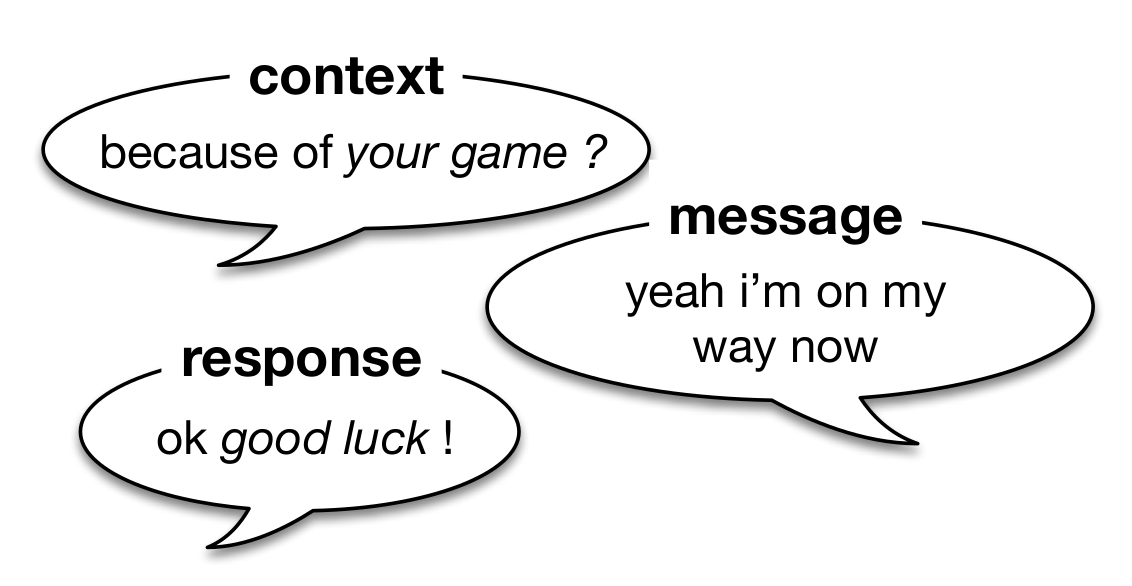
\includegraphics[width=0.6\textwidth]{figure/context_message_response.png}
    \centering
    \caption{上下文,消息和响应的关系\upcite{DCGM}}
    \label{fig:context_message_response}
\end{figure}

% -- Definitions -- %
下面定义面向闲聊的对话系统的主要术语。
本领域考察的场景是两个人交替的用文本(而不是语音)进行对话,
两人有先后顺序的各说一段话$x, y$,称为一轮对话$t = (x, y)$(Turn),
一个对话数据样本$D$是对话的序列$D = t_1, t_2, \dots, t_n$,
它至少包含一轮对话,
样本的最后一轮对话$t_n = (x_n, y_n)$称为当前轮,
序列$t_1, t_2, \dots, t_{n-1}$称为当前轮的上下文$c$,
$x_n$称为当前轮的消息$m$,$y_n$称为当前轮的响应$r$(在不引起歧义的情况下,“当前轮”可以省略)。
若样本只有一轮对话,则上下文为空序列。
$c,m,r$三者的关系如图~\ref{fig:context_message_response}~所示。
给定上下文$c$和消息$m$,模型需要预测响应$r$,
这就是对话响应生成问题(Dialogue Response Generation)。


% -- Generative System -- %
面向闲聊的对话系统又可以分为生成式系统(Generative System)和检索式系统(Retrieval System)
\upcite{corpus_survey,NUC},
两者的主要区别是产生输出的机制不同。
简单来说,如果一个系统能生成训练集里没有出现过的句子,
就把它称为生成式系统,反之则称为检索式系统\upcite{HowNot}。
生成式系统估计了给定输入特征$X$,预测结果为$Y$的条件概率$p(Y|X)$,
并输出使条件概率最大化的句子。
设$U$是所有句子的集合,生成式模型的输出机制可以表示为:
\begin{align}
    Y = \argmax_{Y'\in U} p(Y'|X)
\end{align}

% -- Retrieval System -- %
检索式系统根据输入特征$X$和数据集$C$中的候选输出$Y'$计算评分$\textit{Score}(X, Y')$,
并选出评分最高的候选。
为了使输出自然流畅而且不容易出现重复,$C$通常由大量人类撰写的语句组成。
常见的评分机制有
词频-逆文档频率(Term Frequency Inverse Document Frequency,TF-IDF)
和语义相似度(Semantic Similarity)等等。
检索式系统的输出机制可以表示为:
\begin{align}
    Y = \argmax_{Y'\in C} \textit{Score}(Y', X)
\end{align}

这两种方法各有优劣:检索式系统的输出没有语法错误并且可以对输出内容进行限制\upcite{NUC},但是不能生成新句子;
生成式系统可以生成新的句子\upcite{Shang},但是容易生成过短的句子\upcite{AdverEval}。
两种系统的联合体(Ensemble)通常能比单一系统获得更好的性能\upcite{Two_are_better_than_one}。
而在实验中,检索式系统也经常作为生成式系统的基线\upcite{Shang,DCGM}。

% -- Short Review of Technical Background -- %
生成式模型的流行得益于自然语言处理领域的一系列基础技术,包括
能为把单词转化为平滑的向量特征的词嵌入(Word Embedding)\upcite{NNLM,word2vec,Glove},
能更有效的对序列建模的循环神经网络语言模型(Recurrent Neural Networks Language Model,RNNLM)\upcite{RNNLM},
能避免梯度消失问题\upcite{VanishingGradient}的门单元,
如长短期记忆(Long Short-Term Memory,LSTM)\upcite{LSTM}和
带门循环单元(Gated Recurrent Unit,GRU)\upcite{GRU},
能端对端训练的序列到序列框架(Sequence to Sequence Framework,Seq2Seq)\upcite{Seq2Seq,GRU},
以及能改善长期依赖问题(Long-Span Dependency)的注意力机制\upcite{JointTransAlign,EffectiveAttention}。

% -- Chatbots Based on Seq2Seq -- %
这些技术促进了基于神经网络的机器翻译(Neural Machine Translation,NMT)的发展,
也促使学者们把机器翻译的技术应用到生成式对话上。
在国外,最早把Seq2Seq框架用到生成式对话的是Vinyals等人\upcite{GoogleChatbot},
他们在OpenSubtitles\upcite{opensub}
上训练的模型能回答简单的常识问题,
并且比基于规则的系统CleverBot\footnote{\url{http://www.cleverbot.com/}}获得了更高的人类评分。

% -- Li -- %
Li等人在增加响应的多样性方面做了一系列的工作。
他们提出把最大互信息作为解码的目标函数\upcite{MMI},
增加消息-响应和响应-消息两个方向的相关性。
他们提出的Persona模型\upcite{persona}在解码器端加入了说话人身份(Speaker ID),
有效的促进了响应的人格一致性(Personality Coherence)。
他们还把强化学习(Reinforcement Learning,RL)和
对抗生成网络(Generative Adversarial Networks,GAN)应用到响应生成问题上\upcite{deep_RL,Adversarial},
并取得了有意义的进展。

% -- Serban -- %
Serban等人扩展了Sordoni等人提出的多层编解码器\upcite{hred-qs},
并将其应用到对话生成领域\upcite{HRED}。
基于多层编解码器,Serban等人又提出了利用随机隐变量增加对话多样性的隐变量多层编解码器\upcite{VHRED},
以及加入了高层次抽象信息的多精度循环神经网络(Multiresolution Recurrent Neural Networks,MrRNN)\upcite{MrRNN}。

% -- Shang -- %
在国内,Shang等人研究了基于新浪微博数据集的短文本对话生成问题\upcite{Shang},
并提出了以GRU为门单元的编解码器模型(Neural Response Machine,NRM)。
他们的模型在人类评价上取得了比检索式系统和基于统计机器翻译
(Statistical Machine Translation,SMT)的系统更好的成绩。
Xing等人提出了能利用主题词的Seq2Seq模型\upcite{Topic_Aware},
由于篇幅有限,不能一一介绍。


\section{课题研究意义}\label{sec:research_meaning}
本领域目前面临两个难题:
一是如何合理评价生成式系统的性能\upcite{HowNot,Shang,deep_RL,deltaBLEU,ADEM},
二是如何避免生成单调无意义的响应,增加响应的多样性\upcite{MMI,Distill,Ritter11,DCGM,HRED},
本课题致力于解决第一个难题。
如表~\ref{tab:multiple_valid_responses}~所示,
对于一则给定的消息,合理响应的数量不止一个。
虽然在机器翻译领域,对于源句子的合理翻译也可以有多个,
但是这些翻译必须在语义上和参考大体一致,并且和源句子的语义完全相同,
所以,机器翻译的合理输出之间只存在语法和词法层面的多样性。
而在对话响应生成领域,尽管什么是合理的响应还没有一个明确的定义,
但从直观上来看,对一个消息的回答不应该是该消息的语义重复,
所以合理的响应不需要和消息保持语义一致性。
对合理响应更少的约束条件意味着更大的可能性空间。
这种固有的多样性导致评价响应生成系统比评价机器翻译系统困难。
\begin{table}
    \centering
    \caption{合理的响应不唯一\upcite{RUBER}}
    \label{tab:multiple_valid_responses}
    \begin{tabular}{rl}
        \toprule
        \midrule
        \textbf{消息:} & 为什么不领养一个? \\
        & Why not adopt one? \\
        \textbf{参考:} & 我也想领养,但是不好找。 \\
        & I hope so, but it's hard to find one. \\
        \midrule
        \textbf{响应1:} & 恩,我已经在朋友中找了。 \\
        & I'm looking for one from my friends. \\
        \textbf{响应2:} & 巴比伦是稀有品种。 \\
        & Pappilon is a rare breed. \\
        \textbf{响应3:} & 可以哈。谢谢你的建议。 \\
        & OK, thank you for your advice. \\
        \bottomrule
    \end{tabular}
\end{table}

本文试图通过实验证实评价生成式模型的困难性,并指出导致这种困难性的几个方面的原因。
虽然,目前大多数评价指标尚不具有和人类评价较高的一致性,
但是对它们的研究将有助于理解现有指标的弱点,从而有助于自动化评估的发展。
尽管没有使用人类评价,本文对评价指标、模型和数据集的分析还是取得了有意义的结论。

\section{课题研究内容}\label{sec:reseach_content}
Liu等人发现自动评价指标在非技术性的Twitter对话数据集上和人类评价只有弱相关性,
在技术性的Ubuntu对话数据集上和人类评价没有相关性\upcite{HowNot}。
本文延续Liu等人的工作,
研究了评价指标之间的相关性,以及模型的性能在不同数据集上的迁移能力。

本文以Serban等人在文献\cite{VHRED}的实验中使用的三个模型LSTM,HRED,VHRED为基线,
扩展了Liu等人在文献\cite{HowNot}中考察的两类指标,即基于词重叠的指标和基于词嵌入的指标,
在三个具有代表性的公开数据集,Ubuntu对话数据集,OpenSubtitles和LSDSCC上进行了实验。

\section{论文组织结构}\label{sec:paper_organization}
本文的组织结构如下:
第~\ref{ch:related_work}~章相关工作介绍了生成式模型的基本定义以及指标和数据集的基本情况。
第~\ref{ch:method}~章研究方法介绍了本文的实验框架,模型超参数,数据集预处理和指标参数的选择等等。
第~\ref{ch:experiment}~章实验结果与讨论详细展示了实验数据和结论。
最后一章结论总结了本文的研究成果,提出了若干研究方向。

% MIT License
% 
% Copyright (c) 2019 Cong Feng
% 
% Permission is hereby granted, free of charge, to any person obtaining a copy
% of this software and associated documentation files (the "Software"), to deal
% in the Software without restriction, including without limitation the rights
% to use, copy, modify, merge, publish, distribute, sublicense, and/or sell
% copies of the Software, and to permit persons to whom the Software is
% furnished to do so, subject to the following conditions:
% 
% The above copyright notice and this permission notice shall be included in all
% copies or substantial portions of the Software.
% 
% THE SOFTWARE IS PROVIDED "AS IS", WITHOUT WARRANTY OF ANY KIND, EXPRESS OR
% IMPLIED, INCLUDING BUT NOT LIMITED TO THE WARRANTIES OF MERCHANTABILITY,
% FITNESS FOR A PARTICULAR PURPOSE AND NONINFRINGEMENT. IN NO EVENT SHALL THE
% AUTHORS OR COPYRIGHT HOLDERS BE LIABLE FOR ANY CLAIM, DAMAGES OR OTHER
% LIABILITY, WHETHER IN AN ACTION OF CONTRACT, TORT OR OTHERWISE, ARISING FROM,
% OUT OF OR IN CONNECTION WITH THE SOFTWARE OR THE USE OR OTHER DEALINGS IN THE
% SOFTWARE.

\chapter{相关工作}\label{ch:related_work}
% ------------------ Models ------------------ %
\section{生成式模型}\label{sec:generative_model}

\subsection{定义}\label{subsec:definition}
如公式~\ref{eqn:generative_cond_prob}~所示,
一个生成式模型定义了给定输入序列$X = x_1, x_2, \dots, x_n$,
输出序列$Y = y_1, y_2, \dots, y_m$的条件概率。
如公式~\ref{eqn:generative_train_objective}~所示,
模型在数据集$S$上的训练目标函数就是最大化样本的条件概率。
从定义上看,只要能估计条件概率$p(Y|X)$的模型就是生成式模型。
\begin{align}
    p(Y|X) &= p(y_1, y_2, \dots, y_m|x_1, x_2, \dots, x_n)
    \label{eqn:generative_cond_prob} \\
    \mathcal{L} &= \frac{1}{|S|} \sum_{(Y, X) \in S} \log p(Y|X)
    \label{eqn:generative_train_objective}
\end{align}

% -- RNN -- %
生成式模型需要把一个长度可变的序列$X$映射到另一个长度可变的序列$Y$,且$X$和$Y$的长度可以不相等。
循环神经网络(RNN)为这个问题提供了自然的解决方案。
它的基本思想是:序列由有序的元素组成,每一个时刻(Time Step)输入一个元素,同时更新内部的隐藏状态(Hidden State),然后输出一个元素。
如图~\ref{fig:RNN_unrolled}~所示,
在时间轴上展开的RNN和一般的前馈神经网络(Feed Forward Neural Networks)很相似,不过所有时刻都共享一个权重矩阵$A$,
该矩阵又称为循环矩阵(Recurrent Matrix),它实现了对输入序列的编码。
\begin{figure}[H]
    \centering
    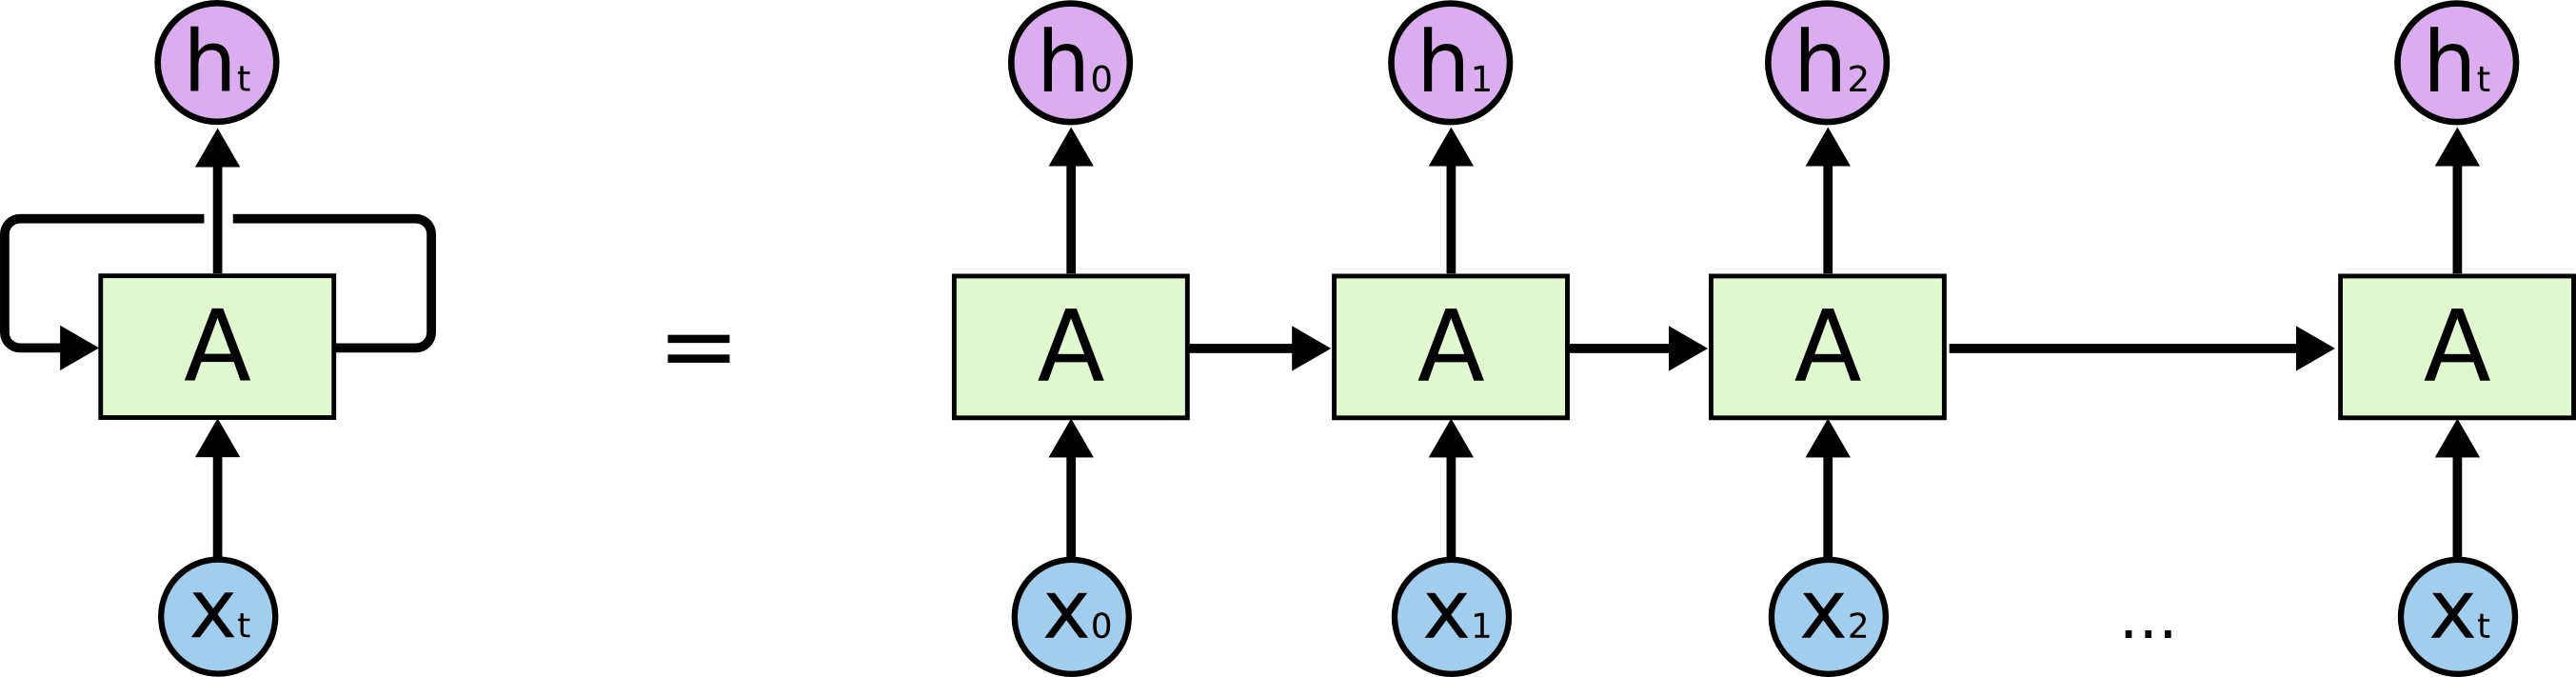
\includegraphics[width=0.6\textwidth]{figure/RNN-unrolled.png}
    \caption{在时间轴上展开的RNN}
    \label{fig:RNN_unrolled}
\end{figure}

% ------------------ RNN types ------------------ %
根据是否使用了某种门单元,RNN可分为普通RNN\upcite{RNNLM},
LSTM\upcite{LSTM}和GRU\upcite{GRU}等等。
根据是否对反向序列(Reversed Sequence)编码,
RNN可分为单向RNN(Unidirectional RNN)
和双向RNN(Bidirectional RNN)\upcite{BiRNN}。
为了更好的处理长期依赖问题,同时避免梯度消失问题的影响,一般采用LSTM或者GRU等有着特殊门单元的RNN。
为了避免梯度爆炸对模型优化的影响,一般采用梯度剪裁(Gradient~Clipping),
对超过某个阈值的梯度进行重置\upcite{GoogleChatbot}。
此外,多层RNN组成的深度循环神经网络比单层RNN有更好的性能\upcite{GoogleChatbot}。

\subsection{RNN语言模型}\label{subsec:RNNLM}
% ---------------- RNNLM ------------------ %
RNN语言模型(Recurrent Neural Network Language Model,RNNLM)
通过循环神经网络估计给定序列$X = x_1, x_2, \dots, x_n$的概率分布:
\begin{align}
    p(X) = \prod_{i=1}^{n} p(x_i|x_1, x_2, \dots, x_{i-1})
    \label{eqn:language_model_probability} \\
    p(x_i = w|x_1, x_2, \dots, x_{i-1}) = \frac{\exp{o_{tw}}}{\sum_{v=1}^V \exp{o_{tv}}}
    \label{eqn:language_model_estimation}
\end{align}

$o_t$是RNN在$t$时刻的输出向量,$V$是词汇表的大小,
一个基于普通RNN的RNN语言模型通过如下公式计算出$o_t$:
\begin{align}
    o_i &= h_i^T W_{out} \\
    h_i &= \sigma \left( x_i^T W_{in} + h_{i-1}^T W_{hh} \right)
\end{align}

$W_{in}$是输入矩阵,$W_{out}$是输出矩阵,$W_{hh}$是循环矩阵,它们都是模型的参数;
$\sigma$是常见的激活函数。
RNN语言模型在训练时最大化训练集上的句子的对数概率:
\begin{align}
    \mathcal{L(X)} = \sum_{i=1}^n \log p(x_i|x_1, x_2, \dots, x_{i-1})
\end{align}

\subsection{Seq2Seq框架}\label{subsec:Seq2Seq}
% ------------------ Seq2Seq ------------------ %
Seq2Seq框架是一种基于RNN的编解码器模型(Encoder-Decoder Model)。
如图~\ref{fig:Seq2Seq}~所示,
Seq2Seq框架使用两个具有独立参数的RNN分别作为编码器和解码器。
首先,编码器把输入序列$X$编码成一个定长向量$v$,
该向量又称为思维向量(Though Vector),
是编码器在最后一个时刻$t_{n}$的隐藏状态。
接着,解码器以$v$为初始隐藏状态生成输出序列。
\begin{figure}[H]
    \centering
    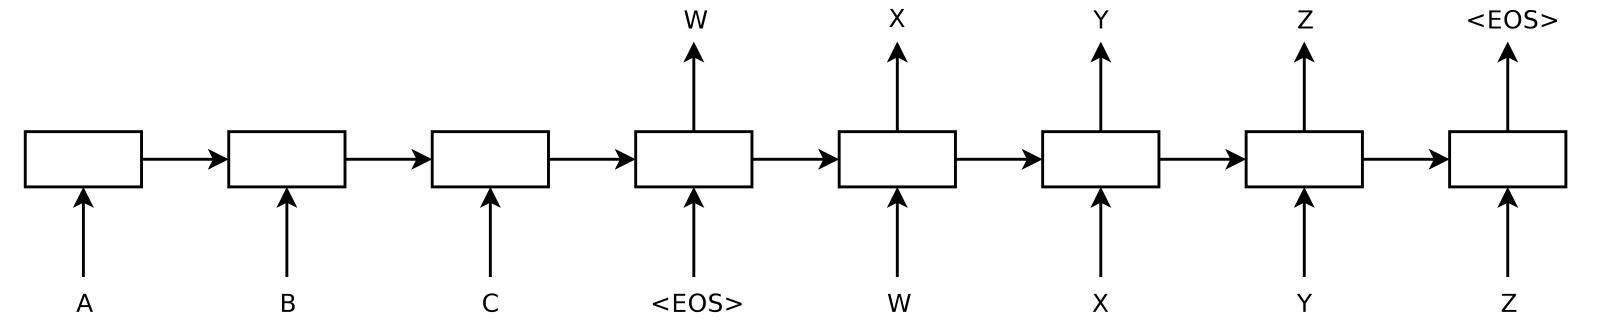
\includegraphics[width=0.8\textwidth]{figure/Seq2Seq.png}
    \caption{Seq2Seq框架图\upcite{Seq2Seq}}
    \label{fig:Seq2Seq}
\end{figure}

通过先把输入序列$X$变换成某种压缩编码$v$,
再把$v$还原为另一个序列$Y$,
Seq2Seq对公式~\ref{eqn:generative_cond_prob}~中的条件概率作了如下分解:
\begin{align}
    p(y_1, y_2, \dots, y_m|x_1, x_2, \dots, x_n) &= \prod_{i=1}^m p(y_i|v, y_1, y_2, \dots, y_{i-1}) \\
    v = h_n, h_i &= f(x_i ,h_{i-1})
\end{align}
$h_n$是编码器的最后一个时刻的隐藏状态,$f$是编码器RNN所使用的门单元的抽象表示。
编码器和解码器以同一个目标函数一起训练。

为了更好的处理长序列,
Seq2Seq一般引入注意力机制(Attention Mechanism)
\upcite{JointTransAlign,EffectiveAttention},
使输入序列的信息不必全部通过固定长度的向量$v$传递。
该机制使解码器能自动关注和当前输出最相关的输入部分,
实现输入序列与输出序列的对自动对齐(Automatic Alignment)。

% ------------------ Decoding ------------------ %
\subsection{解码算法}\label{subsec:decode}
从生成式模型定义的概率分布中产生输出序列的过程称为解码(Decoding)。
生成式模型虽然可以估计任意输入输出对$(X, Y)$的条件概率$p(Y|X)$,
但是对于任意给定输入$X$,所有可能的输出$Y$的数量过于庞大,不可能枚举所有的$Y$并求其中概率最大者。
所以在解码过程中,需要使用某种启发式搜索算法从所有可能的输出中产生一个近似最优解,
这些算法又称为解码算法。
最简单的解码算法是贪心搜索(Greedy Search),
如公式~\ref{eqn:greedy_search}~所示,该算法在每一时刻都选择使当前部分生成的句子的条件概率最大的单词。
因为公式~\ref{eqn:greedy_search}~中的各个$y_i$都不是独立的,
而受之前输出的单词的影响,所以贪心搜索不能保证得到条件概率最大的输出序列。
\begin{align}
    y_i = \argmax_{w \in V} p(w|y_1, y_2, \dots, y_{i-1}, X)
    \label{eqn:greedy_search}
\end{align}

如公式~\ref{eqn:random_sampling}~所示,随机取样(Random Sampling)
在每一时刻都按照模型输出的单词的概率分布随机选取一个单词。
随机取样能在一定程度上避免单调响应的问题\upcite{HRED},
然而在更多时候,它会导致输出中出现语法错误\upcite{DiverseBeam}。
\begin{align}
    p(y_i = w) = p(w|y_1, y_2, \dots, y_{i-1}, X), w \in V
    \label{eqn:random_sampling}
\end{align}

集束搜索(Beam Search)是一种标准的解码算法,
它在生成整个输出的过程中维护一个大小为$B$的列表,称为集束(Beam)。
算法开始时,集束初始化为模型生成的$B$个概率最高的单词。
算法的循环不变式如下:
每一次迭代开始前,集束中都有$B$个部分生成的句子,它们称为候选$Y_c$。
每次迭代,算法对集束中的每一个候选都生成$B$个概率最大的下一个单词$w_{i+1, c}$,
从而形成$B \times B$个部分生成的句子,
它们称为扩展的候选集。
迭代结束时,算法只保留扩展的候选集中前$B$个概率最大的句子。
迭代不断进行直到某些候选中产生了句子结束符号(End-of-Sentence,EOS),
此时算法结束并将这些完成的句子作为输出。
本质上,集束搜索是一种队列长度有限的宽度优先搜索
(Breath First Search)。

% -- Diverse Beam -- %
为了增加模型输出的多样性,学者们提出了许多改进的解码算法。
Li等人提出了Diverse Beam算法\upcite{DiverseBeam},
该算法在标准集束搜索中加入对来自相同父节点的候选的惩罚,
即鼓励来自不同父节点的候选单词。
他们发现来自不同父节点的单词通常比来自相同父节点的单词更具有语义多样性。
% -- MMI -- %
Li等人还提出了以最大互信息(Maximum Mutual Information,MMI)为目标函数的解码算法\upcite{MMI}。
他们训练了一个最大化正向概率$p(Y|X)$的模型和
一个最大化反向概率$p(X|Y)$的模型,
并用反向概率对用正向概率生成的候选句子列表进行重新排序。

% -- Stochastic Greedy Sampling -- %
Li等人还提出了随机贪心取样(Stochastic Greedy Sampling)算法\upcite{Distill},
以求在随机取样和贪心搜索之间找到一个最佳的平衡点。
该算法只在条件概率最高的前$K$个候选单词中随机取样,
参数$K$控制了随机取样和贪心搜索之间的比例:
$K$越大,算法越接近随机取样,$K$越小,算法越接近贪心搜索。
这些改进的解码算法在分别在不同程度上提高了响应的多样性。

% ------------------ Metrics ------------------ %
\section{自动化评价指标}\label{sec:automatic_metric}
\subsection{评价指标简介}\label{subsec:metrics_intro}
机器翻译领域已有大量和人类评价相关性较高的指标,例如
BLEU\upcite{BLEU},
NIST\upcite{NIST},
METEOR\upcite{METEOR},
BEER\upcite{beer},
CHRF\upcite{chrf},
TER\upcite{TER}等等。
然而,适用于开放领域的,面向闲聊的对话系统的指标为数不多。
在考察本领域对自动指标的使用情况之前,先对各种指标作一个简要介绍。

% --------------- BLEU ------------------ %
双语评估指标(Bilingual Evaluation Understudy,BLEU)\upcite{BLEU}是机器翻译领域的经典指标。
它是一个系统层面的评价指标,即评价一个系统在整个测试集上的性能。
BLEU指标只有一个参数$N$,表示要计算的各阶n-gram准确率的最大值;例如$N = 4$表示要计算1-gram到4-gram的准确率。
准确率指的是系统输出和参考输出之间的n-gram重叠数占系统输出总的n-gram的比例。
BLEU由在整个数据集上计算的各阶n-gram准确率的几何平均值(Geometric Mean)和简短惩罚系数(Brevity Penalty)相乘得到。
引入简短惩罚系数的原因是,较短的系统输出句子的准确率较高,需要矫正。
n-gram准确率的计算公式为:
\begin{align}
    p_n = \frac{
    \sum_{\mathcal{C} \in \{\textit{Candidates}\}
    \sum_{\textit{n-gram} \in \mathcal{C}}}
    \textit{Count}_{\textit{clip}}(\textit{n-gram})
    }{
    \sum_{\mathcal{C'} \in \{\textit{Candidates}\}}
    \sum_{\textit{n-gram}' \in \mathcal{C'}}
    \textit{Count}(\textit{n-gram}')
    }
\end{align}
$\textit{Candidates}$为系统输出的句子集合,$\textit{Count}_{\textit{clip}}(\textit{n-gram})$为截断的n-gram共现数,
$\textit{Count}(\textit{n-gram}')$是系统输出中的总n-gram数。
简短惩罚系数BP的计算公式为:
\begin{align}
    \textit{BP} =
    \begin{cases}
        \ 1 \ & \text{if} \  c > r \\
        \ e^{1 - r/c} \ & \text{if} \  c \leq r \\
    \end{cases}
\end{align}
其中$c$是模型输出句子的长度,$r$是参考输出句子的长度。
BLEU的最终公式为:
\begin{align}
    \textit{BLEU} = \textit{BP} \cdot \exp \left( \sum_{n=1}^N w_n \log p_n \right)
\end{align}
实际使用中一般取$N = 4$,$w_n = 1 / N$。
由于原始的BLEU容易在句子层面给出0分,人们提出了各种平滑处理方案\upcite{sBLEU-Smooth}。
本文在使用BLEU时也采用了一种平滑处理。

% ------------ ROUGE -------------- %
面向召回率的摘要评估指标
(Recall-Oriented Understudy for Gisting Evaluation,ROUGE)\upcite{ROUGE}
是自动摘要领域(Automatic Summarization)的经典指标。
它的变形有ROUGE-N,ROUGE-L,ROUGE-W和ROUGE-S等,分别使用了不同的特征,
如n-gram共现数、最长公共子序列(Longest Common Subsequence,LCS)和二元跳词(Skip-Bigram)等。
这些指标的基础是信息检索领域常用的F1得分(F1-score),即准确率和召回率的加权调和平均值:
\begin{align}
    \textit{F1-score} = \frac{(1 + \beta^2) RP}{R + \beta^2 P}
\end{align}
参数$\beta$控制准确率和召回率的相对比例。
下面介绍ROUGE的各种变形,无特殊说明时,当指标是句子层面的时候,$n$是系统句子的长度,$m$是参考句子的长度;
当指标是摘要层面的时候,$n$是系统摘要的总单词数,$m$是参考摘要的总单词数。

ROUGE-N利用了n-gram共现数,其公式为:
\begin{align}
    \textit{ROUGE-N} = \frac{
    \sum_{S \in \{\textit{Reference}\}}
    \sum_{\textit{n-gram} \in S}
    \textit{Count}_\textit{matched}(\textit{n-gram})
    }{
    \sum_{S \in \{\textit{Reference}\}}
    \sum_{\textit{n-gram} \in S}
    \textit{Count}(\textit{n-gram})
    }
\end{align}
摘要层面的ROUGE-N具有相同的形式。

句子层面(Sentence Level)的ROUGE-L的公式为:
\begin{align}
    R_{lcs} &= \frac{\textit{LCS}(X, Y)}{m} \\
    P_{lcs} &= \frac{\textit{LCS}(X, Y)}{n} \\
    \textit{ROUGE-L} &= \frac{(1 + \beta^2) R_{lcs}P_{lcs}}
    {R_{lcs} + \beta^2 P_{lcs}}
\end{align}
$LCS$是两个序列的最长公共子序列的长度。
摘要层面的ROUGE-L的公式为:
\begin{align}
    R_{lcs} &= \frac{\sum_{i=1}^\mu \textit{LCS}_\cup(r_i, C)}{m} \\
    P_{lcs} &= \frac{\sum_{i=1}^\mu \textit{LCS}_\cup(r_i, C)}{n} \\
    \textit{ROUGE-L} &= \frac{(1 + \beta^2) R_{lcs}P_{lcs}}{R_{lcs} + \beta^2 P_{lcs}}
\end{align}
$\mu$是系统摘要的句子数量,
$\textit{LCS}_\cup(r_i, C)$是参考句子$r_i$和候选摘要$C$(由多个句子组成)的LCS的并集。

句子层面的ROUGE-W的公式为:
\begin{align}
    R_{wlcs} &= f^{-1} \left( \frac{\textit{WLCS}(X, Y)}{f(m)} \right) \\
    P_{wlcs} &= f^{-1} \left( \frac{\textit{WLCS}(X, Y)}{f(n)} \right) \\
    \textit{ROUGE-W} &= \frac{(1 + \beta^2) R_{wlcs}P_{wlcs}}{R_{wlcs} + \beta^2 P_{wlcs}}
\end{align}
$\textit{WLCS}$是两个序列的加权最长公共子序列,它奖励连续的最长公共子序列。
摘要层面的ROUGE-W与摘要层面的ROUGE-L类似。

二元跳词是保持在句子中的顺序不变的一对单词,两个单词之间可以有任意数量的其他单词。
基于二元跳词的句子层面ROUGE-S定义为:
\begin{align}
    R_{skip2} &= \frac{\textit{SKIP2}(X, Y)}{C(m, 2)} \\
    P_{skip2} &= \frac{\textit{SKIP2}(X, Y)}{C(n, 2)} \\
    \textit{ROUGE-S} &= \frac{(1 + \beta^2) R_{skip2}P_{skip2}}{R_{skip2} + \beta^2 P_{skip2}}
\end{align}
$C(\cdot, \cdot)$为组合数。
摘要层面的ROUGE-S相当于把摘要看作首尾相连的句子来计算。
ROUGE-SU是ROUGE-S加入了一元词匹配(Unigram Matching)的扩展。

% ----------------- METEOR ----------------- %
基于显式顺序的翻译指标(
Metric for Evaluation of Translation with Explicit ORdering,METEOR)
\upcite{METEOR}是针对BLEU的一些弱点作了改进的机器翻译的指标。
与BLEU相比,METEOR在句子水平上与人类评价有更好的相关性。
METEOR首先计算系统输出和参考输出之间的一元词匹配,这些匹配由多个可配置的模块计算产生,
包括严格匹配(Exact),Porter词根匹配(Porter-Stemmer)和WordNet同义词匹配(WordNet-Synonymy)等等。
接着,METEOR在一元词匹配上计算一个对齐,并得到准确率和召回率,进而得到F1得分:
\begin{align}
    \textit{Fmean} = \frac{10PR}{R + 9P}
\end{align}
METEOR还加入了对较短的n-gram匹配的惩罚系数:
\begin{align}
    \textit{Penalty} = 0.5 * \left( \frac{\#chunks}{\#unigrams\_matched} \right)
\end{align}
$\#unigrams\_matched$是所有匹配的一元词的数量;
一元词匹配的长度越短,$\#chunks$就越大。
METEOR的最终公式为:
\begin{align}
    \textit{METEOR} = \textit{Fmean} * (1 - \textit{Penalty})
\end{align}

% --------- Perplexity ------------ %
困惑度(Perplexity,PPL)是一种衡量统计语言模型性能的指标。
困惑度为$P$意味着一个模型在预测一个单词的时候,平均需要从大约$P$个单词中等可能的选出一个。
因此,困惑度越低,语言模型在选择一个单词时就越不“困惑”。
困惑度的计算公式为:
\begin{align}
    \textit{Perplexity} = \frac{1}{\#\textit{words}} \exp(-\frac{1}{N} \sum_{i=1}^N \log p(x_i))
\end{align}
$\#words$是样本的总单词数,
$N$是用于测试的样本数,$x_i$是一个样本,在语言模型中它是一个句子,
在生成式模型中它是一对输入输出序列$(X, Y)$;
$p(x_i)$是模型估计的概率,
一个好的模型应该对测试集的样本(正样本)给出较高的概率。

% --------- embedding based ------------ %
基于词嵌入的指标是一类基于分布式假设
(Distributed Hypothesis)\upcite{distributed_hypothesis,Mathematical_structures_of_language},
用分布式语义(Distributed Semantic)来衡量两个句子的相似程度的指标。
它们常用于句子文本相似性(Sentence Textual Similarity)和学生输入自动打分\upcite{GreedyAndOptimal}等任务中。
这类指标一般用某种组合方式从句子的词向量中得到句子的向量表示,
再用余弦相似度(Cosine Similarity)测量两个句子向量的相似程度\upcite{VectorCompose},
如公式~\ref{eqn:cosine}~所示:
\begin{align}
    \text{cos}(x, y) = \frac{x\cdot y}
    {\left\| x \right\| \cdot \left\| y \right\|}
    \label{eqn:cosine}
\end{align}
最常见组合方式是对词向量取平均值,类似于词袋表示(Bag-of-Words),对应的指标就是向量平均值(Vector Average):
\begin{align}
    \bar{e_r} &= \frac{\sum_{w \in r} e_w}{|\sum_{w' \in r} e_{w'}|} \\
    \textit{Vector-Average} &= \cos(\bar{e_r}, \bar{e}_{\hat{r}})
\end{align}
$r$是参考输出,$\hat{r}$是系统输出,$w$是句子中的一个单词。

另外一种组合方式是向量极值(Vector Extrema),
它把词向量每个维度上的极端值作为句子向量在该维度上的值\upcite{Vector_Extrema}:
\begin{align}
    \text{extrema}(d_i) &=
    \begin{cases}
        \ \max d_i & \text{if}\ \max d_i \geq |\min d_i| \\
        \ \min d_i & \text{otherwise}
    \end{cases} \\
    e_r^{ex} &= [\text{extrema}(d_1), \dots, \text{extrema}(d_n)] \\
    \textit{Vector-Extrema} &= \cos( e_r^{ex}, e_{\hat{r}}^{ex} )
\end{align}
$[\cdot, \cdot]$表示连接多个标量形成一个向量,
$e_r^{ex}$是参考输出的向量极值表示,$e_{\hat{r}}^{ex}$是系统输出的向量极值表示。

贪心匹配(Greedy Matching)
得名于加权二部图(Weighted Bipartite Graph)的最大匹配问题\upcite{GreedyAndOptimal}:
把两个句子的单词看做一个二部图的所有节点,任意两个节点之间有一条边,定义该边上的权重为两个单词的余弦相似度。
问题是:如何构造一个匹配,使其中的边的权重之和最大。贪心匹配给出了一种贪心算法:
\begin{align}
    G(r, \hat{r}) = \frac{
    \sum_{w \in r} \max_{\hat{w} \in \hat{r}} \cos(e_w, e_{\hat{w}})
    }{ |r| } \\
    \textit{Greedy-Matching} = \frac{
    G(r, \hat{r}) + G(\hat{r}, r)
    }{2}
\end{align}
关于基于词嵌入的指标,值得指出的是:除了上述三种组合方法外,还有很多其他方法\upcite{VectorCompose}。

% -------- Distinct-N ---------- %
如公式~\ref{eqn:distinct_n}~所示,Distinct-N是Li等人提出的衡量句子n-gram多样性的指标\upcite{MMI},
$\#\textit{unique-ngrams}$是句子中不重复的n-gram数量,$\#\textit{words}$是句子的总单词数。
\begin{align}
    \textit{Distinct-N} = \frac{\#\textit{unique-ngrams}}{\#\textit{words}}
    \label{eqn:distinct_n}
\end{align}

% ------- ADEM ------------ %
Lowe等人提出了基于神经网络的自动化对话评价模型
(Automatic Dialogue Evaluation Model,ADEM)\upcite{ADEM}。
如图~\ref{fig:ADEM_model}~所示,
ADEM采用VHRED的多层编码器分别对上下文$c$,参考$r$和响应$\hat{r}$
进行编码,然后简单的将三者的编码线性组合到一起,并经过归一化,得到落在区间$[1, 5]$的得分。
模型通过最小化和人类评价的均方误差(Mean Squared Error,MSE)端对端的训练。
\begin{figure}[H]
    \centering
    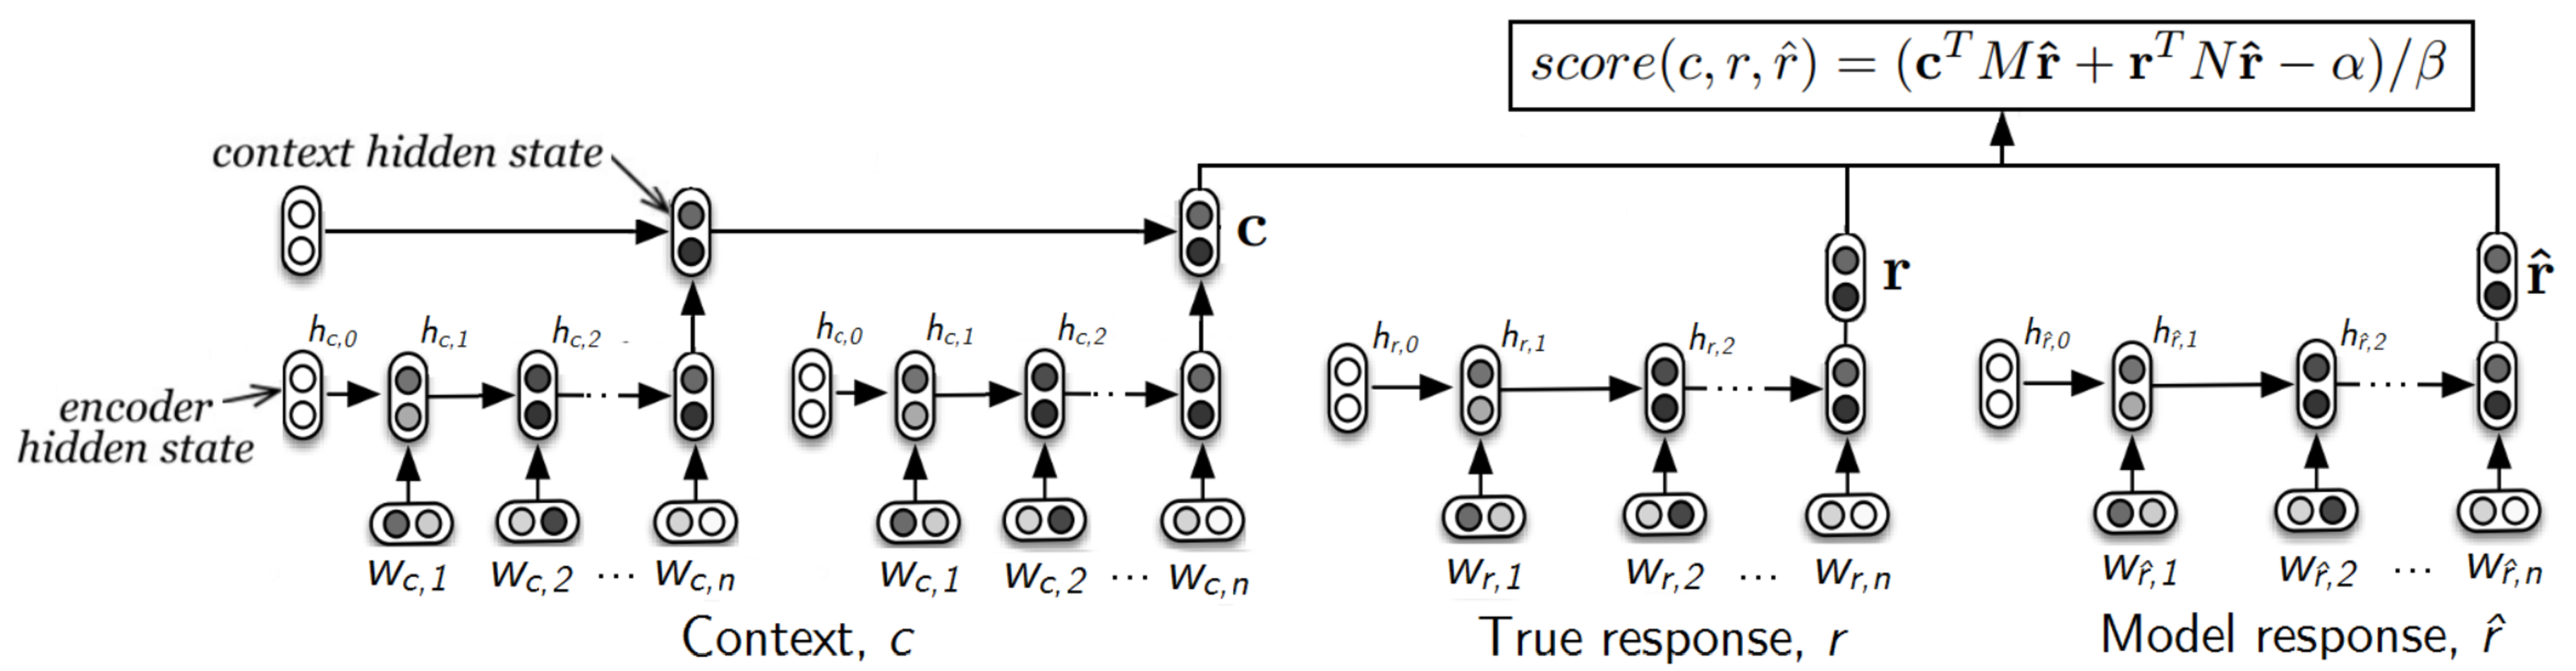
\includegraphics[width=0.9\textwidth]{figure/ADEM.pdf}
    \caption{ADEM模型结构图}
    \label{fig:ADEM_model}
\end{figure}

公式~\ref{eqn:ADEM_score}~是ADEM的打分公式,$M, N$是可学习的
参数矩阵,$\alpha, \beta$是缩放常量,使得分落在$[1, 5]$区间。
如公式~\ref{eqn:ADEM_objective}~所示,
模型的训练目标函数是一个带L2正则化的均方误差。
\begin{align}
    \textit{score}(c, r, \hat{r}) = (c^T M \hat{r} + r^T N \hat{r} - \alpha) / \beta
    \label{eqn:ADEM_score} \\
    \mathcal{L} = \sum_{i=1:K} [\textit{score}(c_i, r_i, \hat{r}_i) - \textit{human}_i]^2 + \gamma \left\| \theta \right\| _2
    \label{eqn:ADEM_objective}
\end{align}
ADEM在一个带人类评价的Twitter数据集上训练并评估,
它的打分和人类评价的相关性在句子水平和系统水平都达到了较高水平。

% ------ RUBER --------- %
Tao等人提出了带参考和无参考的混合指标
(Referenced Metric and Unreferenced Metric Blended Evaluation Routine,RUBER)\upcite{RUBER}。
如图~\ref{fig:RUBER_components}~所示,
RUBER由带参考的指标(Referenced Score)和无参考的指标(Unreferenced Score)两部分组成。
带参考的指标使用
基于词嵌入的最大-最小池化(Max-Min Pooling)作为句子向量,
衡量了消息和响应的相似度,公式如下:
\begin{align}
    v_{max}[i] = \max \{ w_1[i], w_2[i], \dots, w_n[i] \} \\
    v_{min}[i] = \min \{ w_1[i], w_2[i], \dots, w_n[i] \} \\
    v = [v_{max}; v_{min}] \\
    s_R(r, \hat{r}) = \cos(v_r, v_{\hat{r}}) =
    \frac{v_r^T v_{\hat{r}}}{\left\| v_r \right\| \cdot \left\| v_{\hat{r}} \right\|}
\end{align}

无参考的指标通过如图~\ref{fig:RUBER_unref_model}~所示的神经网络估计响应和消息的相关程度。
该模型用负采样(Negative Sampling)训练,不需要人类评价作为监督信号。
RUBER在中文数据集豆瓣\footnote{\url{http://www.douban.com}}上取得了较高的人类评价相关性。
\begin{figure}[H]
    \begin{subfigure}{0.45\linewidth}
        \centering
        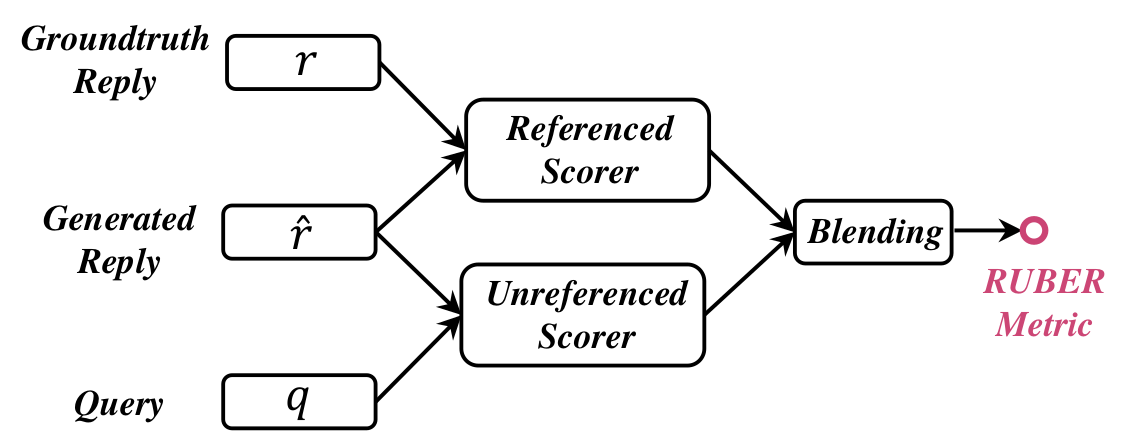
\includegraphics[width=\linewidth]{figure/RUBER_overview.png}
        \caption{RUBER的分数组成}
        \label{fig:RUBER_components}
    \end{subfigure}%
    \begin{subfigure}{0.45\linewidth}
        \centering
        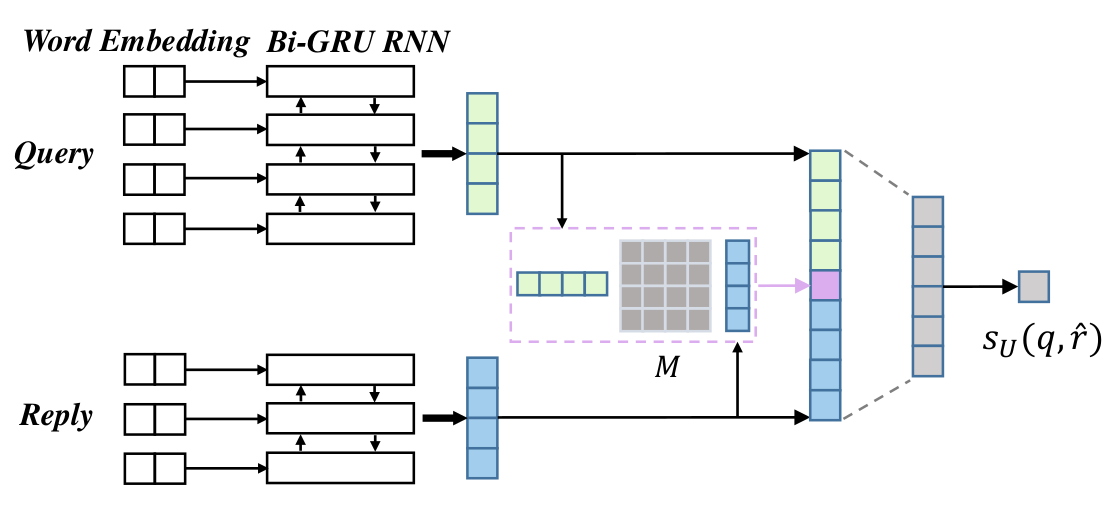
\includegraphics[width=\linewidth]{figure/RUBER_model.png}
        \caption{无参考指标的模型结构}
        \label{fig:RUBER_unref_model}
    \end{subfigure}
    \centering
    \caption{RUBER指标}
\end{figure}

% ------- AdverEval --------- %
Kannan等人初步尝试了基于对抗生成网络的对抗式评价
(Adversarial Evaluation)\upcite{AdverEval}。
他们训练了一个鉴别器(Discriminator)来区分一个响应是来自系统还是来自人类,
并且发现鉴别器能捕捉到基于Seq2Seq的模型倾向于生成短句子和通用句子的缺点。
基于相似的思路,Li等人在文献\cite{Adversarial}中构建了完整的对抗生成网络,
提出了训练和评价的整体框架。
关于对抗生成网络的内容超出了本文的范围,所以不再描述。

% -- Usage of Metrics -- %
\subsection{评价指标的使用情况}\label{subsec:metrics_usage}
生成式对话系统还没有公认的合适的评价指标。
学者们很早就意识到了这一点\upcite{Ritter11,GoogleChatbot,Shang,HRED},
所以他们常常使用人类评价作为核心的评判标准,有时用指标来衡量模型某一方面的特性,
但很少把指标作为评价系统的主要手段。
除了人类评价和指标,
展示并分析模型的输出也是衡量模型性能的常见方法,通常称为定性分析(Qualitative Analysis)。
表~\ref{tab:qualitative_analysis}~展示了模型GoogleChatbot对哲学问题的响应,
从中可以看出该模型对哲学问题的回答具有一定的语义相关性。
\begin{table}
    \centering
    \caption{定性分析的例子\upcite{GoogleChatbot}}
    \label{tab:qualitative_analysis}
    \begin{tabular}{ll}
        \toprule
        \midrule
        \textbf{人类:} & what is the purpose of life ? \\
        \textbf{模型:} & to serve the greater good .\\
        \midrule
        \textbf{人类:} & what is the purpose of living ? \\
        \textbf{模型:} & to live forever . \\
        \midrule
        \textbf{人类:} & what is the purpose of existence ? \\
        \textbf{模型:} & to find out what happens when we get to the planet earth . \\
        \midrule
        \textbf{人类:} & where are you now ? \\
        \textbf{模型:} & i' m in the middle of nowhere . \\
        \midrule
        \textbf{人类:} & what is the purpose of dying ? \\
        \textbf{模型:} & to have a life . \\
        \midrule
        \textbf{人类:} & what is the purpose of being intelligent ? \\
        \textbf{模型:} & to find out what it is . \\
        \midrule
        \textbf{人类:} & what is the purpose of emotions ? \\
        \textbf{模型:} & i don' t know . \\
        \bottomrule
    \end{tabular}
\end{table}

% Ritter -- MT-chat
Ritter等人首次尝试了数据驱动的,面向闲聊的对话响应生成\upcite{Ritter11}。
因为不清楚面向任务的指标能不能用于评价生成式模型,
他们就使用了亚马逊众包平台(Amazon Mechanical Turk,AMT)的人工评价。
他们利用人类评价的数据考察了BLEU在这方面的适用性,
并发现BLEU的系统层面得分非常低,和人类评价的相关性也不是很高。
据此他们认为BLEU不能直接应用到本领域。

% Shang -- NRM
Shang等人在评价他们的模型时分析了几种指标在本领域的适用性\upcite{Shang}。
他们认为BLEU并不适用,因为合理的响应的空间太大了,参考响应不可能完全覆盖到;
而常用于评价语言模型的困惑度也不适用,因为它不能测量响应的自然程度及其对消息的相关程度。
最后他们选择了人类评价。

% Sordoni -- DCGM-1-2
Sordoni在评价他们的模型时采用了BLEU和METEOR两种指标\upcite{DCGM}。
为了处理庞大而多样的响应空间,他们用信息检索(Information Retrieval,IR)的方法从数据集中挖掘潜在的合理响应,
并让人类评估员对其合适度(Appropriateness)打分,
从而构造了一个多重参考测评集(Multiple-Responses Benchmark Dataset)。
在这样的测评集上,他们发现BLEU对系统的排名和人类评价非常一致。
这种构建方法也见于LSDSCC\upcite{LSDSCC}的测试集的构造,
以及DeltaBLEU\upcite{deltaBLEU}指标的设计思路。

% Serban -- HRED
Serban等人在HRED模型的评价中使用了困惑度和单词分类错误(Word Classification Error,WCE)\upcite{HRED}。
他们认为困惑度是适用的,因为在存在多个合理输出的情况下,困惑度总是衡量生成单一参考输出的概率,
这意味着它能可靠的衡量模型的质量。
单词分类错误是模型的输出中正确预测的单词占整个数据集的单词的比例。
这里的“正确预测”要求单词在句子中的顺序也要正确,所以它比困惑度更严苛。
尽管使用了自动化指标,
Serban等人指出:这些指标与语法正确度(Grammatical Correctness)
和语义连贯度(Semantic Coherence)之间的相关性并不明确。
值得注意的是,他们并没有使用人类评价。

% Serban -- VHRED
Serban等人在VHRED模型的评价中使用了基于词嵌入的指标\upcite{VHRED}和人类评价。
他们认为,虽然基于词嵌入的指标和人类评价的相关度不高,
但是它们可以衡量话题相似性(Topic Similarity),
即模型的响应和参考之间的语义是否相似。
他们用人类评价和定性分析验证了基于词嵌入的指标所衡量的话题相似性。

% Vinyals -- Google Chatbot
Vinyals等人在评价他们的模型时使用了困惑度,定性分析和人类评价\upcite{GoogleChatbot}。
尽管他们的模型在上述评价中都打败了基线模型,
但是他们认为这些评价方法都存在许多弊端。
能快速并且准确的评价系统性能的指标仍有待学界研究。

% -- Dataset -- %
\section{开放领域的对话数据集}\label{sec:public_dataset}
本领域所使用的数据集一般称为开放领域的对话数据集(Open-Domain Dialogue Corpus)。
和传统的面向任务的数据集相比,它们的话题广泛,语法形式多样,
而且常带有非自然语言符号(表情符号,URL等等)\upcite{corpus_survey}。
表~\ref{tab:dataset_list}~列举了一些常见的数据集,
其中大规模是指样本数量在1M及以上的,
中等规模是指样本数量在50K--1M之间的\footnote{1K = 1024,1M = 1024 K,1G = 1024 M。}。
除了新浪微博数据集(Sina Weibo Corpus)是中文数据集外,其他都是英文数据集。
与Twitter相关的数据集由于隐私保护政策的原因,不能公开原始数据。
数据集\upcite{supreme,wiki_pages,tennis_corpus,parliamentary,
gone_awry,movie_dialogs_corpus,DailyDialog}都具有元信息,
如时间戳,对话双方身份信息等等。
数据集\upcite{DailyDialog,LSDSCC,DCGM}都有人类标注信息,
如情感、话题和方面(Aspect)等。
元信息和人类标注信息提供了额外的表征,对构建更智能的对话系统很有帮助。
\begin{table}
    \centering
    \caption{开放领域的对话数据集}
    \label{tab:dataset_list}
    \begin{tabular}{llll}
        \toprule
        名称 & 规模 & 领域 & 是否公开 \\
        \midrule
        Ubuntu Dialogue Corpus\upcite{ubuntu_corpus} & 大 & 技术支持 & 是 \\
        Twitter Corpus\upcite{Ritter11} & 大 & 短文本多领域闲聊 & 否 \\
        Twitter Triple Corpus\upcite{DCGM} & 大 & Twitter Corpus的扩展版本 & 否 \\
        OpenSubtitles\upcite{OPUS,opensub} & 大 & 电影字幕(Subtitles) & 是 \\
        LSDSCC\upcite{LSDSCC} & 中 & Reddit论坛电影板块 & 是 \\
        Supreme Court Corpus\upcite{supreme} & 中 & 美国高等法院辩论 & 是\\
        Wikipedia Talk Pages Corpus\upcite{wiki_pages} & 中 & 维基百科编辑者在线讨论 & 是 \\
        Tennis Corpus\upcite{tennis_corpus} & 中 & 网球比赛赛后新闻发布会 & 是 \\
        Parliament Corpus\upcite{parliamentary} & 中 & 国会讨论 & 是 \\
        Conversations Gone Awry Corpus\upcite{gone_awry} & 中 & 维基百科讨论页面吵架集锦 & 是 \\
        Movie Dialogs Corpus\upcite{movie_dialogs_corpus} & 中 & 电影对白 & 是 \\
        Movie-DiC\upcite{Movie-DiC} & 中 & IMSDB电影对白 & 否 \\
        MovieTriples\upcite{HRED} & 中 & Movie-DiC的扩展版本 & 否 \\
        SubTle\upcite{Luke_SubTle} & 中 & 电影字幕 & 否 \\
        DailyDialog\upcite{DailyDialog} & 中 & 日常对话 & 是 \\
        Sina Weibo Corpus\upcite{weibo} & 中 & 新浪微博短文本闲聊 & 是 \\
        \bottomrule
    \end{tabular}
\end{table}

% -- Conclusion -- %
\section{小结}\label{sec:rw_conclusion}
本文从模型,指标和数据集三个方面回顾了本领域的研究现状。
在模型方面,基于Seq2Seq的对话系统有多种优势,例如:
能够直接生成响应,
能端对端的训练,
能从大量语料数据中自动学习语言规律,减少写死的规则,
能利用话题和情感等多种表征,等等。
然而这类系统也有弊端,
比如无法准确控制生成的内容,
偏向于生成单调的响应,
没有人格一致性等等。

在指标方面,对话系统的指标还不能像机器翻译的指标那样准确的评价系统的性能。
% -- this is totally disscusion.
目前最大的问题可能是如何提高指标和人类评价的相关性。
导致这个困境的核心原因可能是对话的响应具有固有的语义多样性,
这个事实可能导致两个结果:1. 用机器翻译的表征,比如单词层面的n-gram,字符层面的n-gram,
对齐等等,无法有效捕捉语义层面的信息。
2. 单纯使用衡量相似性的指标无法捕捉多样性的维度,从而与人类评价不符。

在数据集方面,本领域已经积累了来自不同领域的数据,例如技术性问答,社交媒体上的闲聊,电影对白和字幕,等等。
一些数据集在领域上出现了重合,
比如电影对话数据集(Movie Dialogs Corpus),
电影三元组数据集(MovieTriples)和Movie-DiC的领域都是电影对白;
OpenSubtitles和SubTle的领域都是电影字幕;
Twitter数据集(Twitter Corpus),
Twitter对话数据集和Twitter三元组数据集的领域都是Twitter短文本闲聊。
% -- This is totally future_work.
尽管人类标注是对话文本的重要补充,但是由于其代价的高昂,
所得的数据量往往比较少;
另一方面,元信息是一类在数据采集过程中伴随对话文本同时获得的描述性信息,
比如对话者的性别(Gender)和角色(Character)等等。
相比与人类标注,元信息更容易获取,规模不受限制。
并且,人类标注和元信息都有助于模型生成更加多样和连贯的响应
\upcite{persona,Topic_Aware,ECM}。
因此,数据集的收集过程应该充分保留原始数据中的元信息,
对话系统应该充分利用元信息。
同时,还应该发展从对话文本中无监督的提取元信息的方法。

\chapter{研究方法}\label{ch:method}

\section{实验框架}\label{sec:eval_framework}
% -- Purposes of Experiment -- %
目前,学界普遍认为自动评价指标和人类评价没有很强的相关性\upcite{HowNot},
但是不同指标之间的一致性还没有得到充分的研究。
另一方面,生成式对话系统在不同数据集上的迁移能力(Transferability)
也是一个研究的比较少的问题。
开放领域的对话数据集所具有的大量噪音,
多样的话题和较弱的语法正确度对模型质量的影响应该引起学者们的重视。
通过实验,本文试图对上述问题进行初步的考察,
具体来说,本文试图回答以下问题:
\begin{enumerate}
    \item 模型的性能是否可以在不同数据集之间保持?
    \item 不同的指标在评价同一个数据集上的模型时有没有一致性?
    \item 模型和数据集,哪一个对得分的影响较大?
\end{enumerate}

% -- Terms and Definitions -- %
本文的实验涉及在多个数据集上训练多个模型,
然后用多种指标测量系统层面得分和句子层面得分。
表~\ref{tab:experiment_triples}~展示了实验所使用的模型,数据集和指标。
记模型的集合为$M$,数据集的集合为$D$,指标的集合为$S$,
为了避免术语上的模糊,本文指明:
一个模型$m \in M$指的是一种生成式模型的体系结构,而不是指一个训练好的模型实例。
一个数据集$d \in D$是指某个领域的全部对话的一个子集,它本身又被分为训练集,验证集和测试集三个子集,
一个指标$s \in S$是指一种能把上下文$c$,
参考$r$和响应$\hat{r}$映射为一个实数的函数$f_s(c, r, \hat{r})$。
在不引起歧义时,在数据集$d$上训练指的是在$d$的训练集上训练,
在数据集$d$上解码指的是在$d$的测试集上解码,
把模型$m$在数据集$d$上完成了训练的实例记为$(m, d)$。

% -- Framework -- %
如图~\ref{fig:framework}~所示,
本文的实验首先让每一个模型$m$在每一个数据集$d$上训练,
并让训练好的模型实例$(m, d)$在$d$上解码产生响应$r$,
然后用每一个指标$s \in S$给$r$在句子层面打分,给$(m, d)$在系统层面打分,
分别得到$\lambda_{u}$和$\lambda_{s}$。
一组实验的最终结果是一个5元组$(m, d, s, \lambda_{s}, \lambda_{u})$,
表示在数据集$d$上训练的模型$m$在指标$s$
的评价下所得的系统层面得分$\lambda_s$和句子层面得分$\lambda_u$。

% -- Data Analysis -- %
本文用pandas\footnote{\url{https://pandas.pydata.org/}}装载实验数据,
用seaborn\footnote{\url{http://seaborn.pydata.org/}}进行数据可视化。
系统层面得分的数据由$(m, d, s, \lambda_s)$四元组组成,
$m, d, s$都是类别变量(Categorical Variable),
$\lambda_s$是数值变量(Numerical Variable)。
由于数据中的类别变量较多,
可视化采用面向类别变量的柱形图和箱体图。
本文用柱形图详细分析了不同模型在不同数据集和指标上的系统得分。
但是,某些模型在某些数据集上的得分过于接近,柱形图难以区分各个模型得分的高低。
于是本文分别从数据集和模型两个维度绘制了箱体图,加强了得分在某个维度上的区分程度。
这些箱体图作为辅助分析方法,放在附录~\ref{ch:dataset_system_dist}。

句子层面的得分$\lambda_u$是一个数值变量,
本文采用频数分布直方图进行分析。
一组待分析的句子层面得分是一个$n$维实值向量: $U_{(m, d, s)} = x_1, x_2, \dots, x_n$,
$n$是测试集的样本数,$(m, d, s)$是模型,数据集和指标组成的三元组,$x_i$是某个样本的得分。
句子层面得分可以看做是从一个分布的数学形式未知的总体的取样,
可以使用无参估计法之一的核密度估计(Kernel Density Estimation,KDE)来估计总体的分布。
句子层面得分比系统层面得分的粒度更细,数据也更多了,为了分析的效率,
本文选择了案例分析,
固定$m = m', d = d'$,分析所有指标在$(m', d')$上的情况。
附录~\ref{ch:metric_dist}~呈现了完整的数据。

\begin{table}[H]
    \centering
    \caption{实验对象一览}
    \label{tab:experiment_triples}
    \begin{tabular}{|r|m{0.6\textwidth}|}
        \hline
        模型 & HRED,LSTM,VHRED \\
        \hline
        数据集 & Ubuntu,OpenSubtitles,LSDSCC \\
        \hline
        指标 & BLEU,ROUGE,METEOR,Vector-Average,
        Vector-Extrema,Greedy-Matching,
        ADEM,PPL,Distinct-N \\
        \hline
    \end{tabular}
\end{table}

\begin{figure}[H]
    \centering
    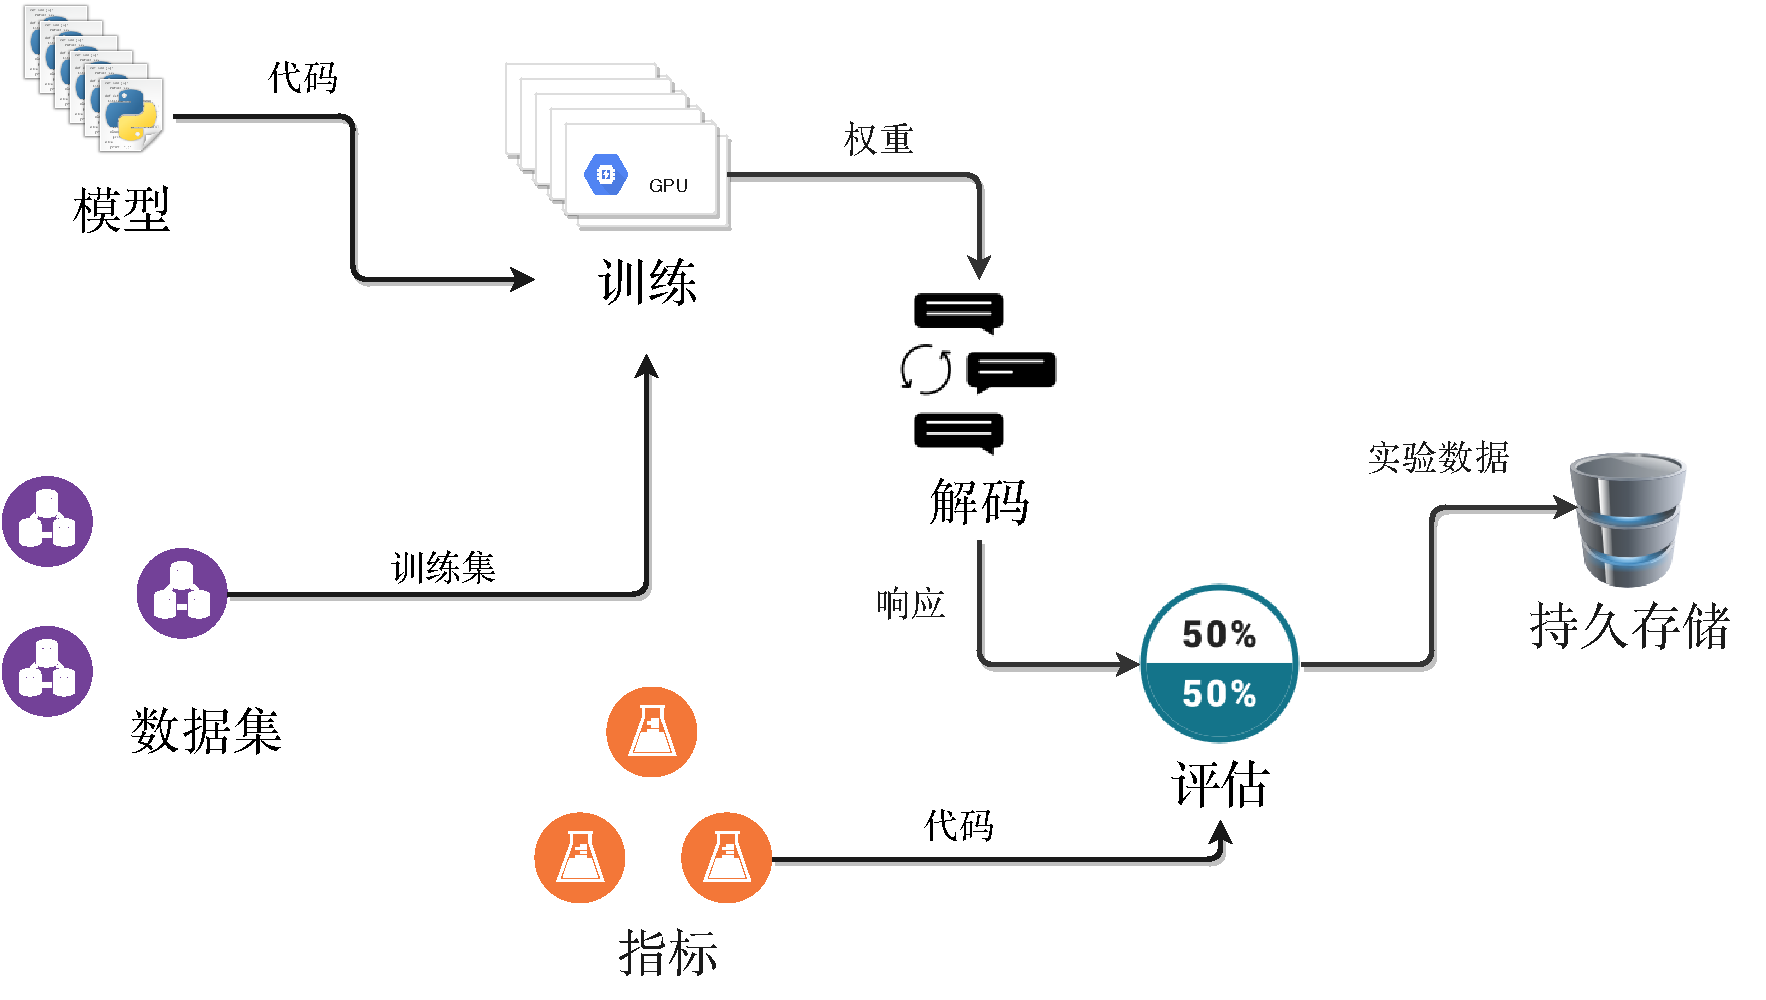
\includegraphics[width=0.8\textwidth]{figure/drawio/eval_v4.pdf}
    \caption{实验框架}
    \label{fig:framework}
\end{figure}

\section{模型选取}\label{sec:model_selection}
第~\ref{ch:related_work}~章已经介绍了生成式模型的基本概念和数据集,指标的基本情况。
和相对有限的数据集和指标相比,生成式模型的数量众多,
由于时间有限,
本文把考察的范围限定在基于Seq2Seq框架的生成式模型上。
Serban等人在文献\cite{HRED,VHRED,MrRNN}
中分别提出了HRED,VHRED和MrRNN模型,
它们是Seq2Seq框架在体系结构上的扩展。
这些模型都各具特色\upcite{A_Short_Review}:
HRED能利用长期对话历史,
VHRED能捕捉对话中的不确定性(Uncertainty)和歧义性(Ambiguity),
MrRNN能生成带有高层次组合结构(Compositional Structure)的响应。
而且,HRED和VHRED都分别在Ubuntu对话数据集和
Twitter三元组数据集上取得了不错的成绩,
说明它们在迁移能力方面是比较强的基线。
是否基于Seq2Seq框架和迁移能力是本文选择模型的两大依据,
HRED和VHRED很好的符合了本文的需求。

本文没有选取普通Seq2Seq模型作为基线,
而是选取了Serban等人使用的基线LSTM模型。
这是为了让实验设置尽可能接近Serban等人的设置,方便复现本文的实验;
本文把加入普通Seq2Seq模型作为以后的工作。
下面详细介绍LSTM,HRED和VHRED三个模型。

% show the power of Serban
\subsection{LSTM模型}\label{subsec:LSTM}
LSTM是一种改进的循环神经网络,用于解决长时间依赖问题\upcite{LSTM}。
LSTM用多个门结构代替了普通RNN中隐藏矩阵$W_{hh}$。
\begin{align}
    f_t &= \sigma(W_f \cdot [h_{t-1}, x_t] + b_f) \\
    i_t &= \sigma(W_i \cdot [h_{t-1}, x_t] + b_i) \\
    \hat{C}_t &= \tanh(W_C \cdot [h_{t-1}, x_t] + b_C) \\
    C_t &= f_t \times C_{t-1} + i_t \times \hat{C}_t \\
    o_t &= \sigma(W_o \cdot [h_{t-1}, x_t] + b_o) \\
    h_t &= o_t \times \tanh(C_t)
    \label{eqn:LSTM_formula}
\end{align}

在公式~\ref{eqn:LSTM_formula}~中,
$x_t$是$t$时刻的输入,
$h_{t-1}$是$t-1$时刻的隐藏状态,
$C_{t-1}$是$t-1$时刻的单元状态(Cell State),
$f_t$是遗忘门(Forget Gate)的输出,
$i_t$是输入门(Input Gate)的输出,
$o_t$是输出门(Output Gate)的输出;
$W_f, W_i, W_o$是三个门的权重矩阵,
$b_f, b_i, b_o$是三个门的偏置向量,
$h_t$是通过一系列门运算后得出的$t$时刻的隐藏状态。
图~\ref{fig:LSTM_structure}~直观的
展现了LSTM内部各个门的连接方式和数据的流动,
LSTM正是通过这些复杂的门运算实现对较长的序列的记忆。
\begin{figure}[H]
    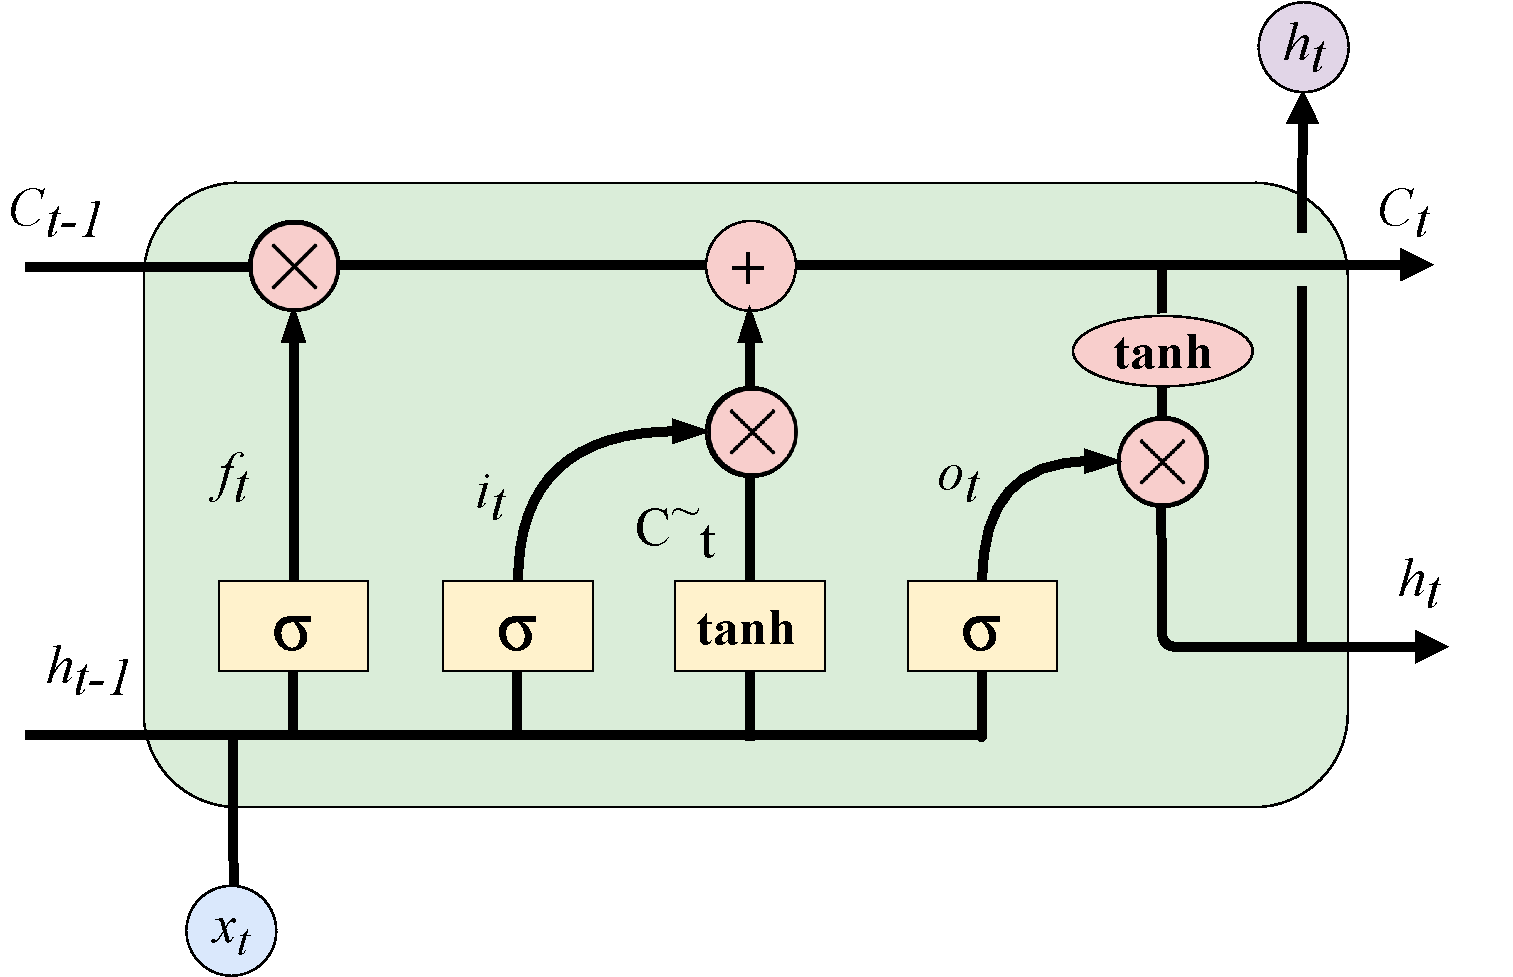
\includegraphics[width=0.5\textwidth]{figure/drawio/LSTM_v9.pdf}
    \centering
    \caption{LSTM内部结构图}
    \label{fig:LSTM_structure}
\end{figure}

如图~\ref{fig:LSTM_IO}~所示,
作为语言模型的LSTM与作为生成式模型的LSTM在数据的输出输出方式上有所不同。
作为语言模型时,输入数据为一个序列$X$,
模型需要重建概率$p(X)$,
在$t_0$时刻,模型输入一个特殊的句子开始符号(Start-of-Sentence),
在$t$时刻,模型的输入$x_t$是$t-1$时刻的输出$y_{t-1}$,
模型的输出$y_t$将和$X$序列的第$t$个元素$X_t$对比,并进行梯度下降。
作为生成式模型时,
输入数据是一对序列$(X, Y)$,
模型需要重建条件概率$p(Y|X)$,
在$t$时刻,模型的输入是$X$序列的第$t$个元素,
模型的输出$y_t$将和$Y$序列的第$t$个元素$Y_t$对比,并进行梯度下降。
本文的实验使用的是作为生成式模型的LSTM。
\begin{figure}[H]
    \begin{subfigure}{0.4\linewidth}
        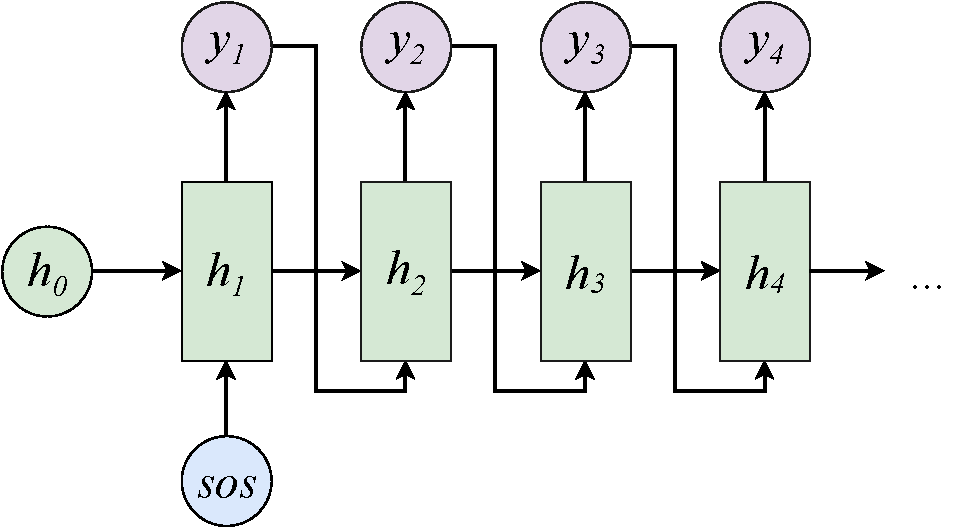
\includegraphics[width=\linewidth]{figure/drawio/RNNLM_lm_v2.pdf}
        \centering
        \caption{语言模型}
        \label{fig:RNNLM_}
    \end{subfigure}%
    \begin{subfigure}{0.4\linewidth}
        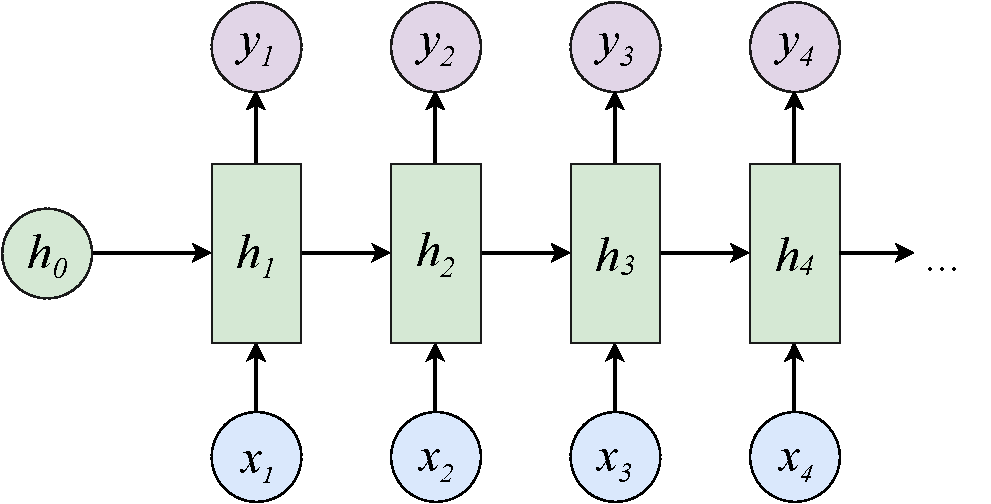
\includegraphics[width=\linewidth]{figure/drawio/RNNLM_generative_v1.pdf}
        \centering
        \caption{生成式模型}
        \label{fig:RNNLM_generative_v1}
    \end{subfigure}
    \centering
    \caption{LSTM模型的两种输入输出方式}
    \label{fig:LSTM_IO}
\end{figure}

\subsection{HRED模型}\label{subsec:HRED}
多层编解码器(Hierarchical Recurrent Encoder-Decoder,HRED)\upcite{HRED}
是一种能利用多轮对话结构的生成式模型。
它把一个对话看做一个两层序列结构,
一个对话$D$由$M$个句子组成:$D = \{ U_1, \dots, U_M \}$,
每个句子由$N_m$个单词组成:$U_m = \{ w_{m, 1}, \dots, w_{m, N_m} \}$。
\begin{figure}[H]
    \centering
    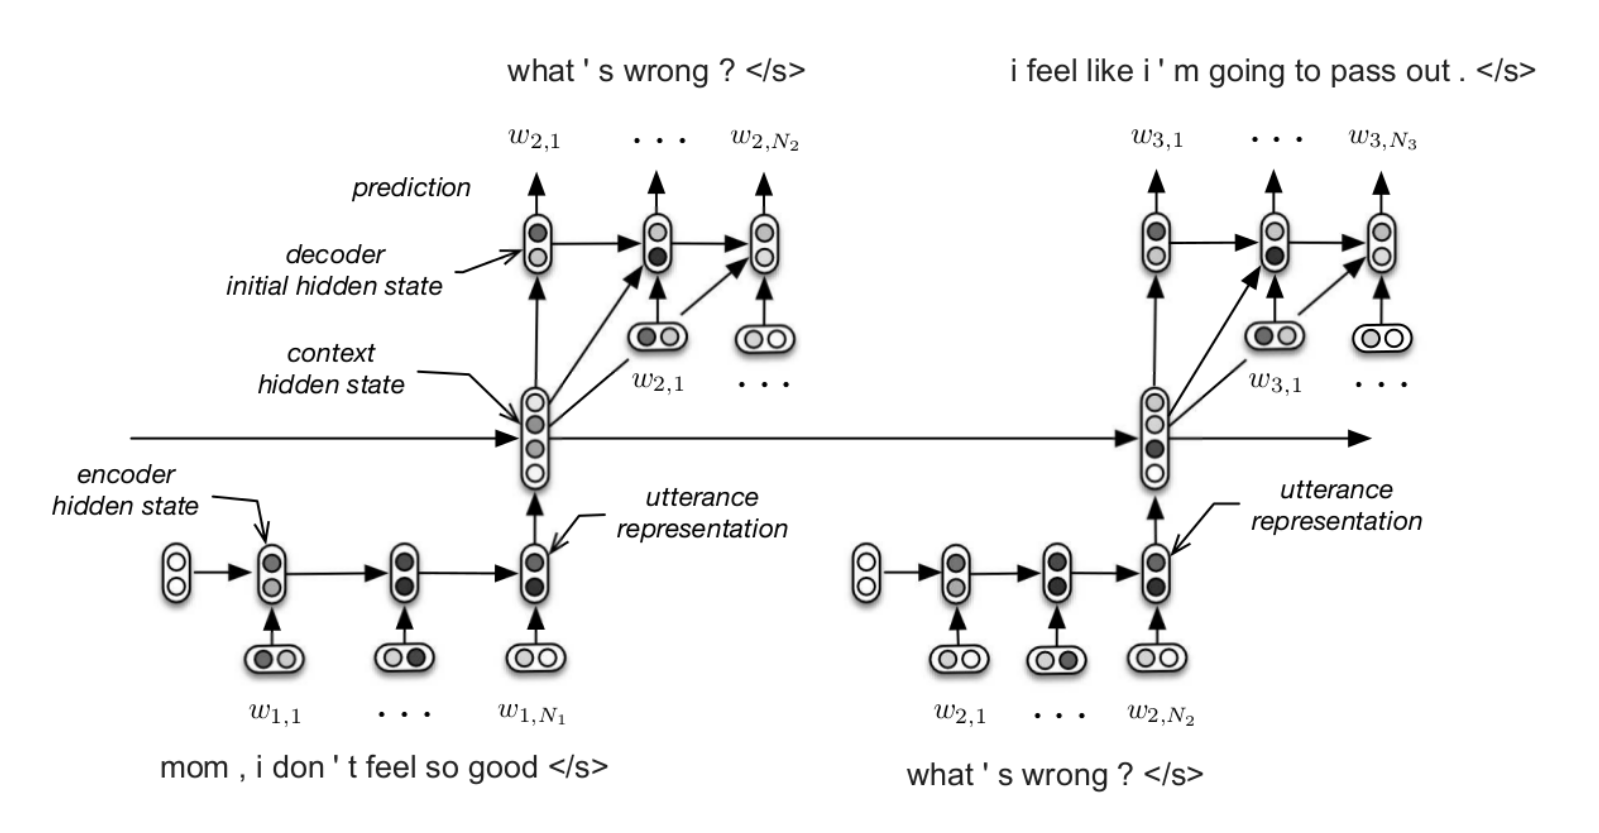
\includegraphics[width=0.8\textwidth]{figure/HRED.png}
    \caption{HRED的计算图\upcite{HRED}}
    \label{fig:HRED}
\end{figure}

如图~\ref{fig:HRED}~所示,
HRED由三个部件组成:
句子编码器(Utterance Encoder)负责把每一个句子编码成一个固定长度的句子向量
(Utterance Vector)$e_u$,
上下文编码器(Context Encoder)负责把$m$个句子向量$e_{u,1}, \dots, e_{u,m}$编码为一个对话向量
(Dialogue Vector)$e_d$,
最后,句子解码器(Utterance Decoder)以对话向量$e_d$为输入,生成对话的下一个句子$U_{m+1}$。
本质上,通过把对话分解为句子的序列,把句子分解为单词的序列,
HRED估计了一个对话$D$的概率$P_{\theta}(D)$:
\begin{align}
    P_{\theta}(D) =
    P_{\theta}(U_1, \dots, U_M) = \prod_{m=1}^M P_{\theta}(U_m|U_{<m})
    = \prod_{m=1}^M \prod_{n=1}^{N_m} P_{\theta}( w_{m, n} |w_{m, <n}, U_{<m} )
\end{align}

$\theta$是HRED模型的参数,
$U_{<m}$表示$U_m$之前的句子序列,
$w_{m, <n}$表示第$m$个句子的第$n$个单词之前的单词序列。

\subsection{VHRED模型}\label{subsec:VHRED}
隐变量多层编解码器
(Latent Variable Hierarchical Recurrent Encoder-Decoder,VHRED)是HRED的扩展,
它在句子解码器中加入了隐随机变量。
如图~\ref{fig:VHRED}~所示,
模型在生成响应时,除了生成对话向量$e_d$外,还产生一个随机变量$z_n$,
并把$z_n$和$e_d$连接到一起作为句子解码器的输入。
随机变量$z_n$能有效增加响应的多样性。
\begin{figure}[H]
    \centering
    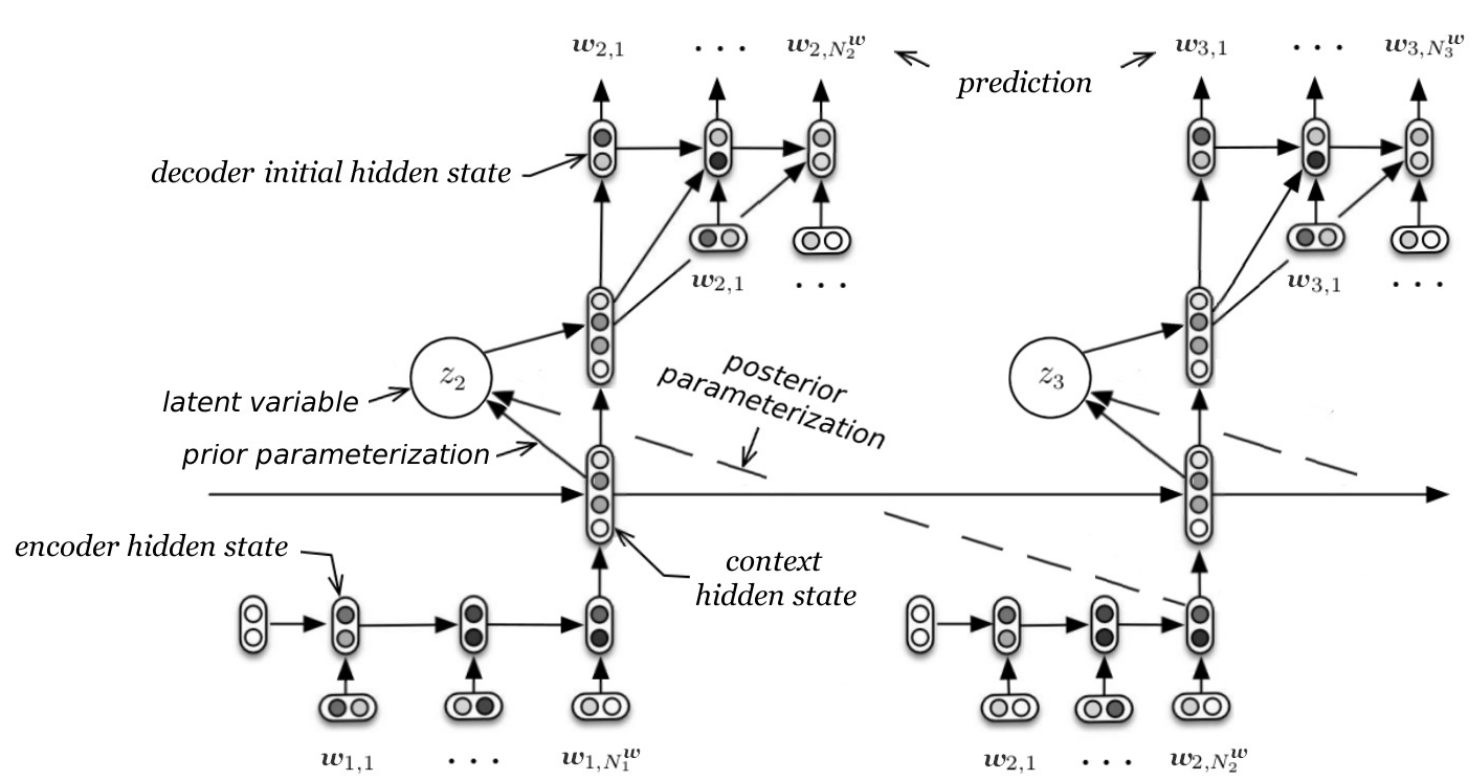
\includegraphics[width=0.8\textwidth]{figure/VHRED.png}
    \caption{VHRED的计算图\upcite{VHRED}}
    \label{fig:VHRED}
\end{figure}

$z_n$服从多元高斯分布
$\mathcal{N}(\mu_{\text{prior}}, \Sigma_{\text{prior}})$,
$\mu_{\text{prior}}$是分布的均值,
$\Sigma_{\text{prior}}$是分布的协方差矩阵,
这些参数
由对话向量经过一个两层的前馈神经网络估计得到。
如公式~\ref{eqn:VHRED_random_variable}~所示,
对于一个对话$D = \{ U_1, \dots, U_M \}$,
每个句子$U_m = \{ w_{m, 1}, \dots, w_{m, N_m} \}$,
模型通过$D$估计了分布
$\mathcal{N}(\mu_{\text{prior}}, \Sigma_{\text{prior}})$。
如公式~\ref{eqn:VHRED_cond_prob}~所示,模型在条件概率
$P_{\theta}(U_n|U_1, \dots, U_{n-1})$
的条件部分加入了随机变量$z_n$,
它的作用可以理解为对话中的高层决策,
比如话题和情感,也可以理解为自然语言的对话中存在的不确定性和歧义性。
模型的训练是通过变分推断(Variational Inference)实现的,
图中的后验参数(Posterior Parameterization)和训练有关。
\begin{align}
    P_{\theta}(z_n|{U}_1, \dots, U_{n-1}) = \mathcal{N}(\mu_{\text{prior}}(U_1, \dots, U_{n-1}), \Sigma_{\text{prior}}(U_1, \dots, U_{n-1}))
    \label{eqn:VHRED_random_variable} \\
    P_{\theta}(U_n|z_n, U_1, \dots, U_{n-1}) = \prod_{m=1}^{M_n}P_{\theta}(U_{n, m}|z_n, U_1, \dots, U_{n-1}, w_{n, 1}, \dots, w_{n, m-1})
    \label{eqn:VHRED_cond_prob}
\end{align}


\section{模型超参数设置}\label{sec:model_hparams}
% ------ Model setup ----------- %
在模型超参数方面,本文的设置和文献\cite{VHRED}大致相同。
本文用Adam\upcite{AdamOpt}来优化所有模型,
一个小批(Mini-batch)处理20个样本。
% -- Dimension of Word Embeddings -- %
本文在Ubuntu上使用维度是300的词嵌入,
在OpenSubtitles和LSDSCC上使用维度是400的词嵌入。
% -- Hidden Units of Utterance Encoder -- %
HRED和VHRED的句子编码器(Utterance Encoder)
在Ubuntu上使用500个隐藏单元,
在OpenSubtitles和LSDSCC上使用1000个隐藏单元。
% -- Hidden Units of Context Encoder -- %
HRED和VHRED的上下文编码器(Context Encoder)
在所有数据集上都使用1000个隐藏单元。
% -- Hidden Units of Utterance Decoder -- %
模型的句子解码器(Utterance Decoder)配置如
表~\ref{tab:utterance_decoder_config}~所示。
% -- Direction of Utterance Encoder -- %
Ubuntu上的模型的句子编码器都使用了单向RNN,
而OpenSubtitles和LSDSCC上的模型的句子编码器则使用双向RNN。
% -- Gate Type of Utterance & Context Encoder -- %
除LSTM外,所有模型的句子编码器和上下文编码器都使用GRU作为门单元。
\begin{table}[H]
    \centering
    \caption{句子解码器的配置情况}
    \label{tab:utterance_decoder_config}
    \begin{tabular}{*{8}{l}}
        \toprule
        \midrule
        & \multicolumn{3}{c}{门单元类型} & & \multicolumn{3}{c}{隐藏状态单元数量} \\
        \midrule
        & HRED & LSTM & VHRED & & HRED & LSTM & VHRED \\
        \midrule
        LSDSCC & LSTM & GRU & GRU & LSDSCC & 1000 & 2000 & 1000 \\
        OpenSubtitles & LSTM & GRU & GRU & OpenSubtitles & 1000 & 2000 & 1000 \\
        Ubuntu & LSTM & LSTM & LSTM & 500 & Ubuntu & 2000 & 500 \\
        \bottomrule
    \end{tabular}
\end{table}

所有的模型都在一台Nvidia GTX上训练了至少1周,
模型收敛时的困惑度如表~\ref{tab:converged_perplexity}~所示。
与文献\cite{VHRED}不同的是,本文没有用预训练的HRED模型来初始化对应的VHRED模型。
所有的模型都使用了梯度剪裁,阈值为1。
所有模型在Ubuntu上的学习率为0.0002,
在OpenSubtitles和LSDSCC上的学习率为0.0001。
在解码时,本文使用随机取样。
\begin{table}
    \centering
    \caption{模型收敛时的困惑度}
    \label{tab:converged_perplexity}
    \begin{tabular}{llll}
        \toprule
        \midrule
        & HRED & LSTM & VHRED \\
        \midrule
        LSDSCC & 32.9229 & 32.5599 & 37.7149 \\
        OpenSubtitles & 41.6392 & 34.2724 & 33.6867 \\
        Ubuntu & 39.1623 & 46.4055 & 40.2486 \\
        \bottomrule
    \end{tabular}
\end{table}

% ------ Dataset Selection ------- %
\section{数据集选取}\label{sec:dataset_selection}
本文选取了三个规模较大,领域具有代表性的数据集,分别是
Ubuntu对话数据集(Ubuntu Dialogue Corpus),OpenSubtitles和LSDSCC数据集,
它们代表了三个常见的对话领域:技术支持,电影字幕和在线论坛。
下面详细介绍这三个数据集。

% --------- Ubuntu ---------- %
Ubuntu对话数据集(下文简称Ubuntu)
是Lowe等人从Freenode IRC网络的Ubuntu板块的聊天日志\footnote{\url{https://irclogs.ubuntu.com/}}
中获取的技术性两人多轮对话。
这个数据集包含了大量技术符号,比如路径,命令,URL,还有笔误(Typo),缩写(Abbreviation)和俚语(Slang)。
它的样本数量多达930,000(接近1M),庞大的数据量为数据驱动的模型提供了极佳的试验场。
它的多轮特性为模型提供了更长的上下文,有助于模型生成更有意义的响应。

% --------- OpenSubtitles -------- %
OpenSubtitles是开源双语数据集项目(The Open Parallel Corpus,OPUS)的一部分。
它是从一个人们可以自由上传和下载电影字幕的网站\footnote{\url{http://www.opensubtitles.org}}的数据库中获取的,
庞大而充满噪音的开放领域数据集,对话数量高达80M。
由于OPUS的目的是收集机器翻译所需要的双语数据集(Parallel Corpus),OpenSubtitles也是一个双语数据集,
它里面并没有对话数据集所需要的轮信息(Turn Information),
而且也没有区分旁白,独白和对白。
Sordoni等人把OpenSubtitles用到对话领域\upcite{GoogleChatbot},
他们把相邻的两个句子分别视为消息和响应,并且每一个句子既是消息又是响应。
Li等人对OpenSubtitles也采用了类似的办法\upcite{MMI,persona,Future,DiverseBeam,
Distill,deep_RL,Adversarial}。

% --------- LSDSCC ------------- %
大规模特定领域对话数据集(A Large Scale Domain-Specific Conversational Corpus,LSDSCC)
是一个特定领域的单轮对话数据集\upcite{LSDSCC}。
它的训练集包含738,095个样本;它的词汇表比较大,达到了50K。
作者从Reddit的电影板块\footnote{\url{https://www.reddit.com/r/datasets}}中获取原始数据,
设计了一套尽可能保留语料信息的清理程序,还使让人类评价员对消息和响应的相关度进行评价,
最终得到一个高质量的消息-响应对数据集(Query-Reply Pair Corpus)。
作者还用信息检索的方法构建了一个多重参考测评集,并基于此提出了一系列衡量响应多样性的指标。

% -- Dataset Preprocessing -- %
\section{数据集预处理}
\label{sec:dataset_proprecessing}
本文使用的Ubuntu对话数据集直接来自Serban等人的项目
\footnote{\url{https://github.com/julianser/hed-dlg-truncated.git}},没有经过任何额外处理。
本文从Li等人的项目
\footnote{\url{https://github.com/jiweil/Neural-Dialogue-Generation.git}}
中获取了经过预处理的OpenSubtitles数据,并作了如下处理:
\begin{enumerate}
    \item 将数据从下标形式还原为单词形式;
    \item 将其词汇表文件\texttt{movie\_25000}转化为下标从0开始的
    pickle格式\footnote{pickle是一种Python特有的序列化格式}。
    \item 用Serban等人的\texttt{convert\_text2dict.py}将训练集,
    测试集和开发集均转换为pickle格式;
    \item 选用OpenSubtitles中的轮数为3,句子最短长度为6的dialogue3\_6子集作为实际使用的数据集;
    \item 由于测试集过大,从中随机抽取1\%的样本作为实验使用的测试集。
\end{enumerate}

本文从作者提供的链接中获取了经过预处理的LSDSCC数据集\footnote{\url{https://drive.google.com/file/d/1nbpbnhwNP14xAc4SAc1 NN5lvEr01dQb/view?usp=sharing}}。
由于它的词汇数量多达50K,为了使内存不溢出,本文将其词汇表裁剪至35000个频率最高的单词。
由于本文只使用单个参考的指标,对LSDSCC的多重参考测评集中的多个参考只取第一个参考。
剩下的处理过程类似OpenSubtitles的处理。

表~\ref{tab:dataset_stats}~是三个数据集的训练集(左)和测试集(右)的统计数据。
从表中可以看到,OpenSubtitles的样本数量要远远超过其他两个数据集,
是Ubuntu的26倍, 是LSDSCC的16倍。
但是,从单词数量来看,OpenSubtitles超过另外两个数据集的倍数却小得多,
这是因为Ubuntu的每一个样本包含了多个句子,
其长度要远远超过OpenSubtitles的样本。
这也导致了Ubuntu的样本数量少于LSDSCC,但是单词数量却超过了LSDSCC。
\begin{table}[H]
    \centering
    \caption{数据集的统计数据}
    \label{tab:dataset_stats}
    \begin{tabular}{*{8}{l}}
        \toprule
        \midrule
        & \multicolumn{4}{c}{训练集} & & \multicolumn{2}{c}{测试集} \\
        \midrule
        数据集 & 词汇数量 & 样本数量 & 单词数量 & 轮数 & 数据集 & 样本数量 & 单词数量 \\
        \midrule
        Ubuntu & 20000 & 448833 & 45697699 & 多轮 & Ubuntu & 18920 & 2045082   \\
        OpenSubtitles & 23876 & 11771393 & 379346841 & 多轮 & OpenSubtitles & 14714 & 474074 \\
        LSDSCC & 35008 & 738095 & 32355628 & 单轮 & LSDSCC & 299 & 10914 \\
        \bottomrule
    \end{tabular}
\end{table}

% -- Metric Config -- %
\section{指标的选择和配置}\label{sec:metric_config}
本文只选择那些生成式对话领域使用过或者提出的指标,
并且尽可能使用业界公认的实现和推荐的参数。
和文献\cite{HowNot}一样,本文只考虑单轮对话和单个参考响应。
% -- BLEU -- %
本文使用NLTK\footnote{\url{https://www.nltk.org/}}提供的BLEU实现,
并且加入了平滑处理。
% -- ROUGE -- %
本文参考了作者的脚本实现了ROUGE,并将准确率和召回率的比例设置为1:9,
因为在机器翻译领域,召回率和人类评价的相关性比准确率高\upcite{METEOR}。
ROUGE-W的权重设置为1.2 。
% -- METEOR -- %
本文使用了METEOR的官方实现\texttt{meteor-1.5.jar},并且按照文档
\footnote{\url{http://www.cs.cmu.edu/~alavie/METEOR/README.html}}的说明,
加入对英语的正则化处理。
% -- PPL -- %
本文使用Serban等人的\texttt{evaluate.py}脚本测量模型的困惑度,
由于该程序对测试样本进行随机取样,从而无法得知某个样本的确切得分,
所以本文只测得了系统层面得分。
% -- EB -- %
关于词嵌入的指标,
本文改写了Serban等人的\texttt{embedding\_metrics.py},
使之能测量句子层面的得分;
和他们一样,本文使用在谷歌新闻数据集(Google News Corpus)上预训练的
word2vec词嵌入\footnote{\url{https://drive.google.com/file/d/0B7XkCwpI5KDYNlNUTTlSS21pQmM}}。
% -- ADEM -- %
关于ADEM指标,本文使用作者提供的代码库
\footnote{\url{https://github.com/mike-n-7/ADEM.git}}
和预训练模型\footnote{\url{https://drive.google.com/file/d/0B-nb1w_dNuMLY0Fad3N1YU9ZOU0/view?usp=sharing}}。
% -- Distinct-N -- %
本文实现了比较简单的Distinct-N指标,
还测量了响应的句子长度$\textit{\#words}$。

\section{小结}\label{sec:method_conclusion}
本章详细介绍了本文的研究方法,包括实验框架,模型的选择和超参数的设置,
数据集的选择和预处理,以及指标的选择和配置。
本章用形式化的语言定义了实验的过程,针对不同形式的实验数据采用不同的分析方法。
由于时间有限,本文从大量的模型和数据集中选取了具有代表性的三个模型和三个数据集,
说明了选择的标准并详细介绍了这些模型和数据集。
在下一章中,本文将展示实验结果并进行讨论。

% MIT License
% 
% Copyright (c) 2019 Cong Feng
% 
% Permission is hereby granted, free of charge, to any person obtaining a copy
% of this software and associated documentation files (the "Software"), to deal
% in the Software without restriction, including without limitation the rights
% to use, copy, modify, merge, publish, distribute, sublicense, and/or sell
% copies of the Software, and to permit persons to whom the Software is
% furnished to do so, subject to the following conditions:
% 
% The above copyright notice and this permission notice shall be included in all
% copies or substantial portions of the Software.
% 
% THE SOFTWARE IS PROVIDED "AS IS", WITHOUT WARRANTY OF ANY KIND, EXPRESS OR
% IMPLIED, INCLUDING BUT NOT LIMITED TO THE WARRANTIES OF MERCHANTABILITY,
% FITNESS FOR A PARTICULAR PURPOSE AND NONINFRINGEMENT. IN NO EVENT SHALL THE
% AUTHORS OR COPYRIGHT HOLDERS BE LIABLE FOR ANY CLAIM, DAMAGES OR OTHER
% LIABILITY, WHETHER IN AN ACTION OF CONTRACT, TORT OR OTHERWISE, ARISING FROM,
% OUT OF OR IN CONNECTION WITH THE SOFTWARE OR THE USE OR OTHER DEALINGS IN THE
% SOFTWARE.

\chapter{实验结果与讨论}\label{ch:experiment}
本文从系统层面得分和句子层面得分两个方面展示了实验的数据与结论。 在众多数据中,本文发现以下主要的结论:
\begin{enumerate}
    \item 同一个数据集上的模型的得分差异较小,不同数据集上的模型得分差异较大。
    \item 各个指标的分布情况呈现集群现象,同一集群内的指标分布相似,不同集群之间的指标分布迥异。
    \item 尽管在某些指标或数据集上一个模型超过另一个模型,但是在全部指标和数据集上,没有哪个模型一致的超过另一个模型。
\end{enumerate}
本文把上述结论归因于以下几个方面:
\begin{enumerate}
    \item 合理的响应的空间巨大,响应具有很高的熵,给评价增加了难度。
    \item 模型在不同数据集上的泛化能力有待加强。
    \item 对话数据集的质量参差不齐,而模型的质量和数据集的质量紧密相关。
\end{enumerate}

% ------------------------- %
% ----- System Level ------ %
% ------------------------- %
\section{系统层面得分}\label{sec:system_scores}
表~\ref{tab:systemScoresAll}~展示了各个模型在不同数据集上测定的各项指标的系统层面得分, 加粗的得分是三个系统中的最优者。 句子平均长度(\#words)没有加粗,因为它是一个参考数据。 从表中的数据来看, 在LSDSCC上HRED取得了除ROUGE-4外所有指标的最优, 在OpenSubtitles上,VHRED取得了除了ADEM和Distinct-N之外所有指标 的最优, 在Ubuntu上情况比较复杂:HRED取得9个指标的最优, LSTM取得了6个指标的最优, VHRED取得了3个指标的最优。 如果把在一个数据集上取得最优指标最多的模型称为在该数据集上的 最优模型的话, 从总体上看,HRED是所有数据集上的最优模型, 因为它在LSDSCC和OpenSubtitles都是最优模型。 但是观察在每一项指标上取得最优的模型时发现, 不同数据集上的取得最优的模型往往不相同。 为了了解不同模型在不同数据集上的表现, 本文对每一个指标的系统层面得分绘制了柱形图。
% MIT License
% 
% Copyright (c) 2019 Cong Feng
% 
% Permission is hereby granted, free of charge, to any person obtaining a copy
% of this software and associated documentation files (the "Software"), to deal
% in the Software without restriction, including without limitation the rights
% to use, copy, modify, merge, publish, distribute, sublicense, and/or sell
% copies of the Software, and to permit persons to whom the Software is
% furnished to do so, subject to the following conditions:
% 
% The above copyright notice and this permission notice shall be included in all
% copies or substantial portions of the Software.
% 
% THE SOFTWARE IS PROVIDED "AS IS", WITHOUT WARRANTY OF ANY KIND, EXPRESS OR
% IMPLIED, INCLUDING BUT NOT LIMITED TO THE WARRANTIES OF MERCHANTABILITY,
% FITNESS FOR A PARTICULAR PURPOSE AND NONINFRINGEMENT. IN NO EVENT SHALL THE
% AUTHORS OR COPYRIGHT HOLDERS BE LIABLE FOR ANY CLAIM, DAMAGES OR OTHER
% LIABILITY, WHETHER IN AN ACTION OF CONTRACT, TORT OR OTHERWISE, ARISING FROM,
% OUT OF OR IN CONNECTION WITH THE SOFTWARE OR THE USE OR OTHER DEALINGS IN THE
% SOFTWARE.

\begin{table}[htb]
    \centering
    \caption{System-Level Scores}
    \small
    \label{tab:system_scores}
    \setlength{\tabcolsep}{0.09cm}
    \begin{tabular}{|l|r|r|r|r|r|r|r|r|r|}
        \hline
        & \multicolumn{3}{c|}{LSDSCC} & \multicolumn{3}{c|}{OpenSubtitles} & \multicolumn{3}{c|}{Ubuntu}\\
        \hline
        & HRED & LSTM & VHRED & HRED & LSTM & VHRED & HRED & LSTM & VHRED\\
        \hline
        ADEM & \textbf{2.6178} & 2.6127 & 2.6163 & \textbf{2.6228} & 2.6224 & 2.6219 & 2.6353 & \textbf{2.6381} & 2.635\\\hline
        BLEU{-}1 & \textbf{0.08} & 0.0726 & 0.0722 & 0.0672 & 0.0638 & \textbf{0.0753} & 0.1314 & 0.1303 & \textbf{0.1365}\\\hline
        BLEU{-}2 & \textbf{0.0264} & 0.0181 & 0.0185 & 0.0171 & 0.0153 & \textbf{0.0264} & 0.0362 & 0.0345 & \textbf{0.0375}\\\hline
        BLEU{-}3 & \textbf{0.0105} & 0.0052 & 0.0066 & 0.0062 & 0.0055 & \textbf{0.0146} & \textbf{0.009} & 0.007 & 0.0089\\\hline
        BLEU{-}4 & \textbf{0.0053} & 0.0 & 0.0028 & 0.0024 & 0.0022 & \textbf{0.01} & \textbf{0.0029} & 0.0018 & 0.0025\\\hline
        Distinct{-}1 & \textbf{0.9577} & 0.9441 & 0.9558 & \textbf{0.973} & 0.9714 & 0.9714 & 0.9074 & \textbf{0.9257} & 0.9113\\\hline
        Distinct{-}2 & \textbf{0.8541} & 0.8511 & 0.8497 & \textbf{0.8669} & 0.8594 & 0.8665 & \textbf{0.9013} & 0.8603 & 0.8968\\\hline
        Greedy & \textbf{0.3303} & 0.3292 & 0.3267 & 0.3102 & 0.2998 & \textbf{0.3145} & \textbf{0.2775} & 0.2364 & 0.273\\\hline
        Average & \textbf{0.5532} & 0.5467 & 0.5483 & 0.5453 & 0.5295 & \textbf{0.5485} & \textbf{0.574} & 0.5205 & 0.5655\\\hline
        Extrema & \textbf{0.2841} & 0.2835 & 0.2814 & 0.3009 & 0.2929 & \textbf{0.3061} & \textbf{0.29} & 0.2663 & 0.2875\\\hline
        METEOR & \textbf{0.0296} & 0.0258 & 0.0281 & 0.0248 & 0.0233 & \textbf{0.0271} & 0.1657 & 0.1635 & \textbf{0.166}\\\hline
        ROUGE{-}1 & \textbf{0.108} & 0.083 & 0.0978 & 0.0784 & 0.075 & \textbf{0.0872} & 0.1644 & \textbf{0.1836} & 0.1683\\\hline
        ROUGE{-}2 & \textbf{0.0226} & 0.0049 & 0.0081 & 0.0053 & 0.0043 & \textbf{0.0107} & 0.0128 & \textbf{0.0143} & 0.0128\\\hline
        ROUGE{-}3 & \textbf{0.0057} & 0.0002 & 0.0035 & 0.0011 & 0.0009 & \textbf{0.0053} & \textbf{0.0007} & 0.0003 & 0.0005\\\hline
        ROUGE{-}4 & 0.0011 & 0.0 & \textbf{0.003} & 0.0002 & 0.0002 & \textbf{0.0038} & \textbf{0.0002} & 0.0 & 0.0001\\\hline
        ROUGE{-}L & \textbf{0.0956} & 0.0681 & 0.0846 & 0.0742 & 0.0707 & \textbf{0.0826} & 0.1493 & \textbf{0.1722} & 0.1535\\\hline
        ROUGE{-}W & \textbf{0.0792} & 0.0537 & 0.07 & 0.066 & 0.0629 & \textbf{0.0734} & 0.1205 & \textbf{0.1391} & 0.1236\\\hline
        PPL & \textbf{32.5599} & 32.9229 & 37.7149 & 41.6392 & 34.2724 & \textbf{33.6867} & \textbf{39.178} & 46.4061 & 40.2641\\\hline
        \#words & 13.1605 & 14.0067 & 12.3612 & 8.807 & 8.6394 & 8.7798 & 23.0646 & 16.4905 & 21.2449\\
        \hline
    \end{tabular}
\end{table}


% -- BLEU -- %
图~\ref{fig:BLEU_system}~是BLEU的系统得分柱形图。 BLEU-1和BLEU-2的情况比较类似: 从总体上看,模型在Ubuntu的得分普遍高于在另外两个数据集上的得分, 而HRED和VHRED在所有数据集上都比LSTM表现好, 在Ubuntu上,VHRED超过了HRED,但在另外两个数据集上, HRED都一致的超过了VHRED。 模型的BLEU-1得分在虽然在不同数据集之间相差较大, 但在同一个数据集内却相差不大。 然而,模型的BLEU-2,BLEU-3,BLEU-4得分即便在同一个数据集内也相差很大。

BLEU-3和BLEU-4的情况比较类似: 从总体上看,没有哪一个数据集的得分要普遍高于其他数据集上的得分。 在所有数据集上,HRED和VHRED的得分仍然普遍比LSTM高, 虽然有时候优势不太明显 。 VHRED在OpenSubtitles上大幅度的超过了HRED, 但在另外两个数据集上,HRED都超过了VHRED。 从绝对数量的角度来看,BLEU的得分随着N的增大而减小, 这是因为两个句子的n-gram共现数随着$N$的增大而减少。
\begin{figure}[H]
    \begin{subfigure}{0.4\linewidth}
        \centering
        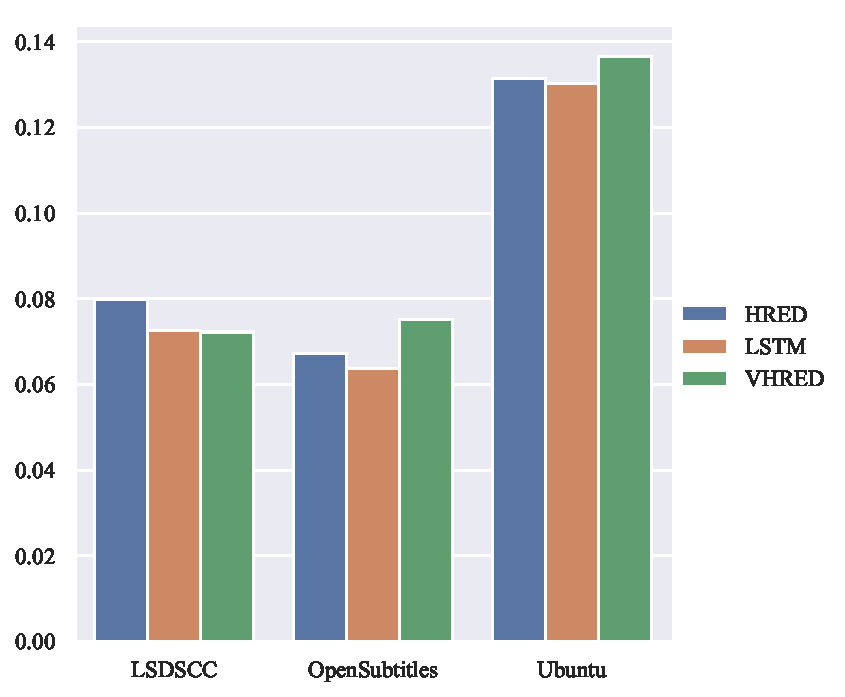
\includegraphics[width=\linewidth]{figure/barplot/bleu_1/plot.pdf}
        \caption{BLEU-1}
    \end{subfigure}%
    \begin{subfigure}{0.4\linewidth}
        \centering
        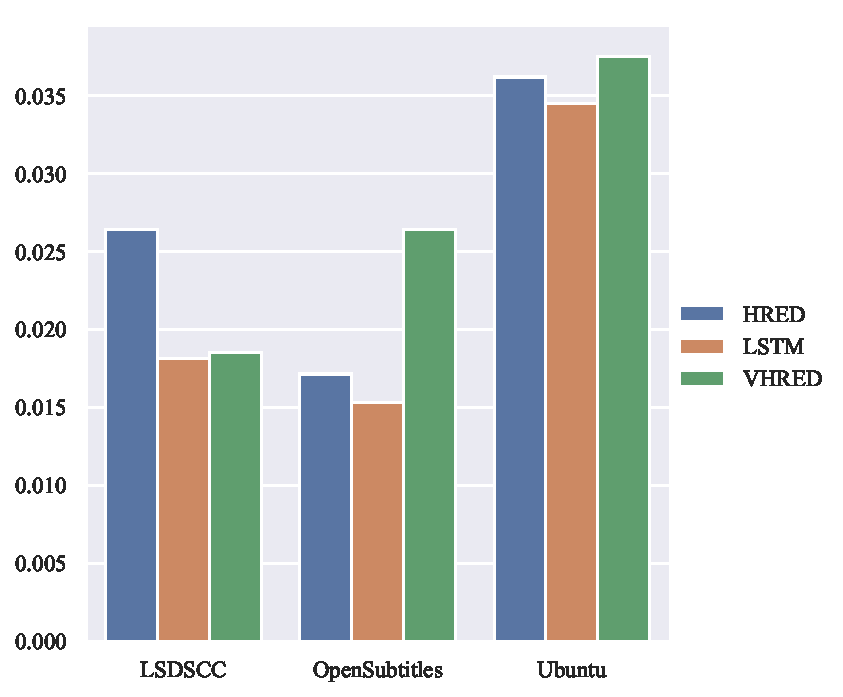
\includegraphics[width=\linewidth]{figure/barplot/bleu_2/plot.pdf}
        \caption{BLEU-2}
    \end{subfigure}
    \begin{subfigure}{0.4\linewidth}
        \centering
        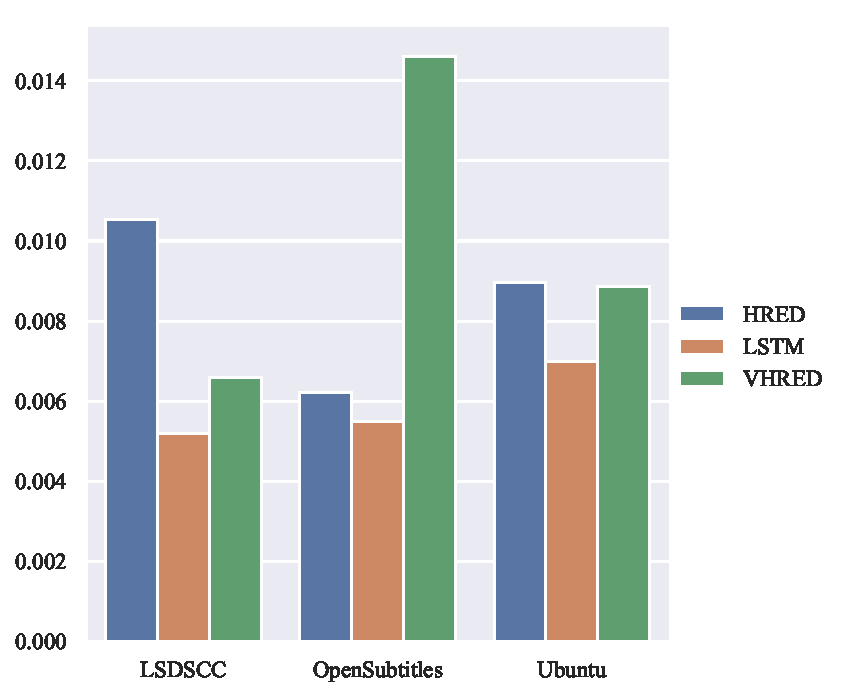
\includegraphics[width=\linewidth]{figure/barplot/bleu_3/plot.pdf}
        \caption{BLEU-3}
    \end{subfigure}%
    \begin{subfigure}{0.4\linewidth}
        \centering
        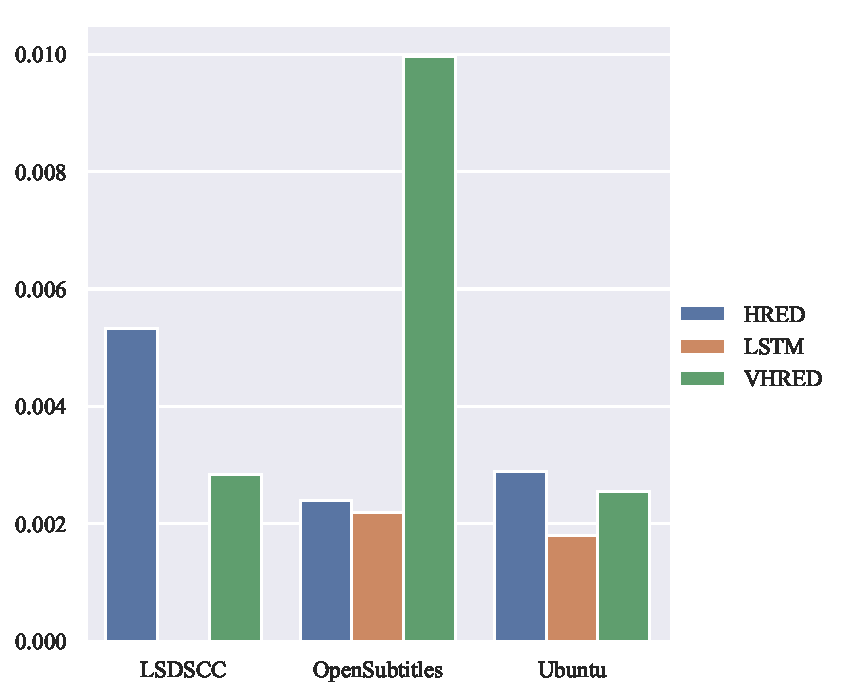
\includegraphics[width=\linewidth]{figure/barplot/bleu_4/plot.pdf}
        \caption{BLEU-4}
    \end{subfigure}
    \centering
    \caption{BLEU的系统得分}
    \label{fig:BLEU_system}
\end{figure}


% -- ADEM_AND_EMB -- %
图~\ref{fig:ADEM_EB_system}~是基于词嵌入的指标和ADEM的系统得分柱形图。 值得注意的是,ADEM对所有数据集上的所有模型的打分都非常接近2.6。 从表~\ref{tab:ADEM_system}~看出, 当数据集不同时,ADEM的分数在百分位变化, 当数据集相同而模型不同时,ADEM的分数在千分位之后(包括千分位)变化, 这表明数据集对ADEM得分的影响要大于模型的影响。
\begin{table}
    \centering
    \caption{ADEM的系统层面打分}
    \label{tab:ADEM_system}
    \begin{tabular}{llll}
        \toprule
        & HRED & LSTM & VHRED \\
        \midrule
        LSDSCC & 2.6178 & 2.6127 & 2.6163  \\
        OpenSubtitles & 2.6228 & 2.6224 & 2.6219 \\
        Ubuntu & 2.6353 & 2.6381 & 2.635 \\
        \bottomrule
    \end{tabular}
\end{table}
从数据集的角度,所有模型在Ubuntu上的得分好于在OpenSubtitles的得分, 而后者要好于在LSDSCC上的得分。 从模型的角度,在LSDSCC上,HRED的得分好于VHRED的得分, 后者要好于LSTM的得分。 在OpenSubtitles上,HRED的得分好于LSTM的得分, 后者要好于VHRED的得分。 在Ubuntu上,最好的模型是LSTM,其次是HRED,最后是VHRED。 从上述分析来看,HRED在两个数据集上得分最优, VHRED在两个数据集上得分最差, LSTM在三个数据集上排名各不相同。 尽管得分的差异很小(最大值和最小值之间只相差0.019), 而且各个数据集上模型的排名都不相同,但是还是可以看出, HRED在ADEM指标上表现较好,而VHRED则较差。 这可能是因为实验中没有用预训练的HRED初始化VHRED。
% MIT License
% 
% Copyright (c) 2019 Cong Feng
% 
% Permission is hereby granted, free of charge, to any person obtaining a copy
% of this software and associated documentation files (the "Software"), to deal
% in the Software without restriction, including without limitation the rights
% to use, copy, modify, merge, publish, distribute, sublicense, and/or sell
% copies of the Software, and to permit persons to whom the Software is
% furnished to do so, subject to the following conditions:
% 
% The above copyright notice and this permission notice shall be included in all
% copies or substantial portions of the Software.
% 
% THE SOFTWARE IS PROVIDED "AS IS", WITHOUT WARRANTY OF ANY KIND, EXPRESS OR
% IMPLIED, INCLUDING BUT NOT LIMITED TO THE WARRANTIES OF MERCHANTABILITY,
% FITNESS FOR A PARTICULAR PURPOSE AND NONINFRINGEMENT. IN NO EVENT SHALL THE
% AUTHORS OR COPYRIGHT HOLDERS BE LIABLE FOR ANY CLAIM, DAMAGES OR OTHER
% LIABILITY, WHETHER IN AN ACTION OF CONTRACT, TORT OR OTHERWISE, ARISING FROM,
% OUT OF OR IN CONNECTION WITH THE SOFTWARE OR THE USE OR OTHER DEALINGS IN THE
% SOFTWARE.

\begin{figure}[H]
    \begin{subfigure}{0.45\linewidth}
        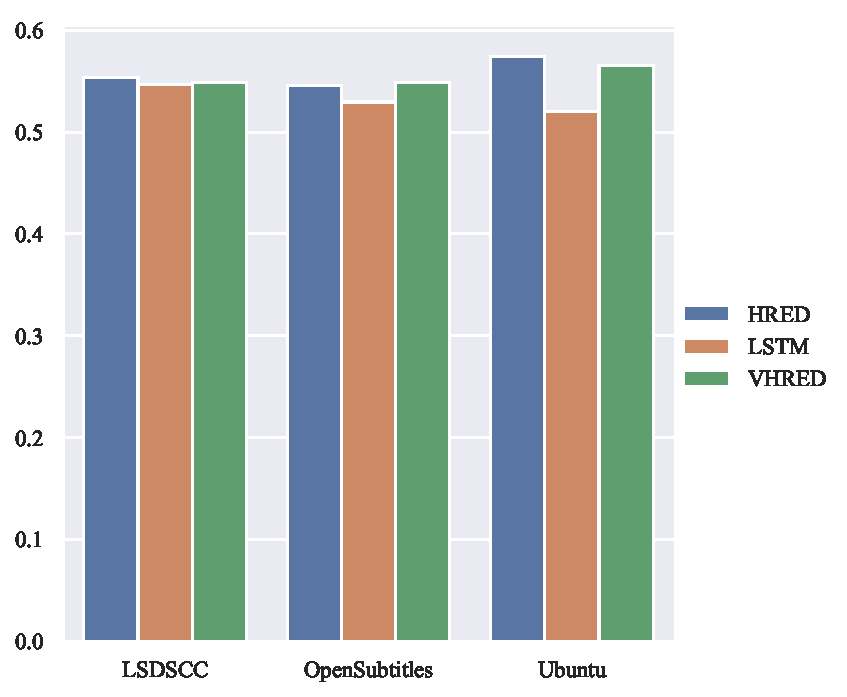
\includegraphics[width=\linewidth]{figure/barplot/embedding_based_vector_average/plot.pdf}
        \centering
        \caption{Average}
    \end{subfigure}%
    \begin{subfigure}{0.45\linewidth}
        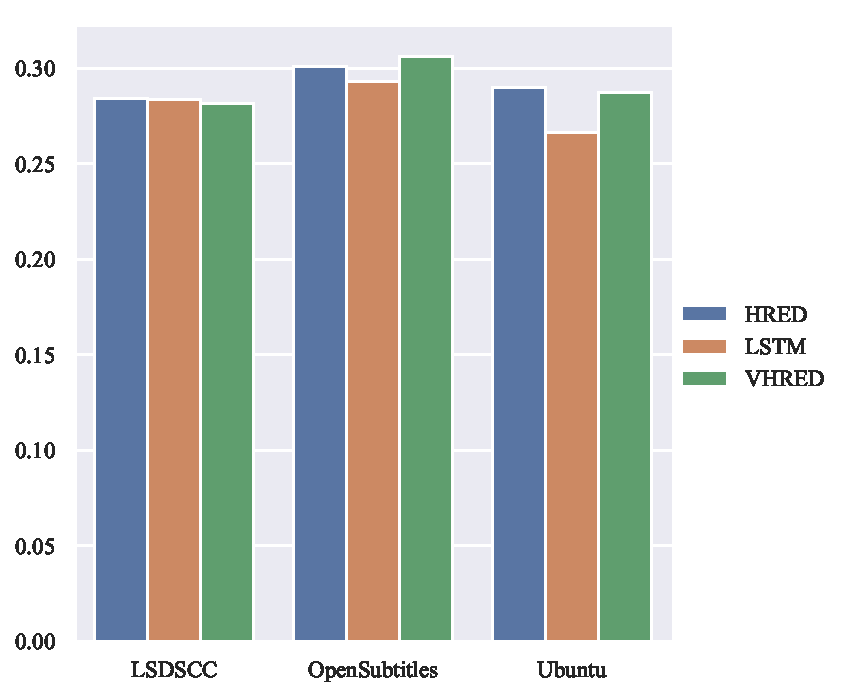
\includegraphics[width=\linewidth]{figure/barplot/embedding_based_vector_extrema/plot.pdf}
        \centering
        \caption{Extrema}
    \end{subfigure}
    \begin{subfigure}{0.45\linewidth}
        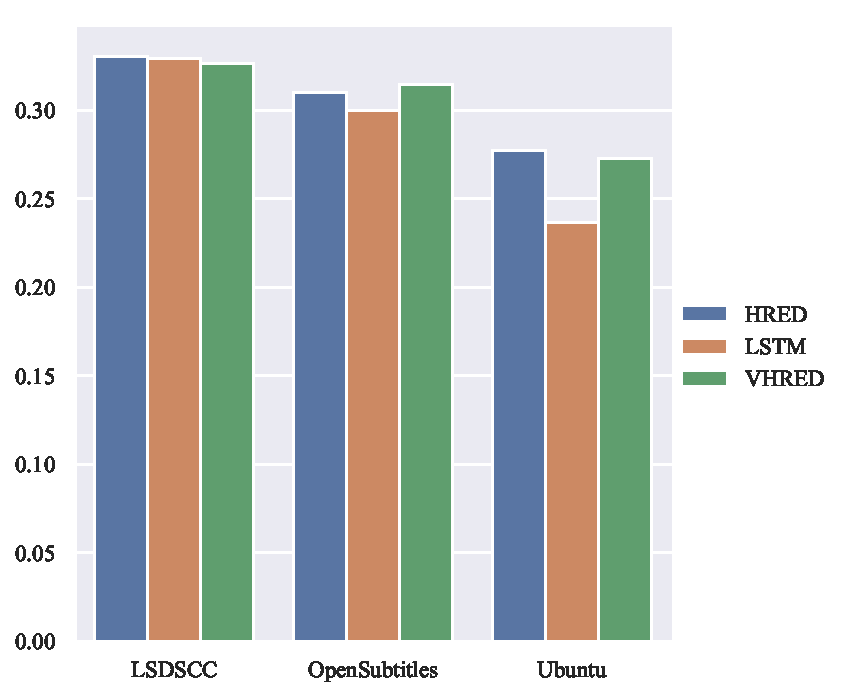
\includegraphics[width=\linewidth]{figure/barplot/embedding_based_greedy_matching/plot.pdf}
        \centering
        \caption{Greedy}
    \end{subfigure}%
    \begin{subfigure}{0.45\linewidth}
        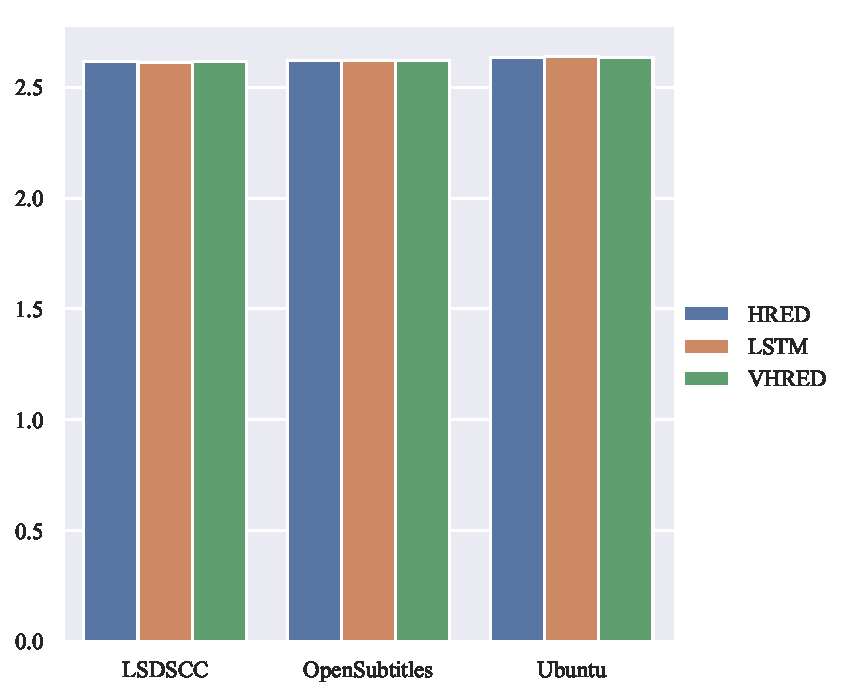
\includegraphics[width=\linewidth]{figure/barplot/adem/plot.pdf}
        \centering
        \caption{ADEM}
        \label{subfig:ADEM_system}
    \end{subfigure}
    \centering
    \caption{基于词嵌入的指标和ADEM的系统得分}
    \label{fig:ADEM_EB_system}
\end{figure}


和ADEM相比,基于词嵌入的指标表现的更具有一致性。 Average,Greedy和Extrema三种指标虽然在绝对数值上有些差异, 但是图像的模式却非常相似。 从总体来看,在所有数据集和指标上,HRED和VHRED都比LSTM表现的好。 在LSDSCC上,这三个指标很难将模型区分开来, 事实上,所有模型在LSDSCC上的某个指标都倾向于得到相同的分数。 基于分析这是因为LSDSCC的测试集样本太少(300个), 没有足够多的样本令模型之间的差异展现出来。 在测试集样本数比较多的OpenSubtitles上,三个模型的区别比较明显, 但是由于OpenSubtitles的噪音比较大,话题比较分散, 模型相对比较容易产生话题相关的响应, 导致三个模型的区分不是特别明显。 在Ubuntu上,三个模型的区分最明显, HRED和VHRED超过了LSTM,拉开了较大距离。 这是因为Ubuntu是一个技术领域的数据集, 含有大量技术词汇,如\texttt{apt-get},\texttt{java}等等。 模型必须能捕捉到消息中的技术相关的语义并生成相关的句子才能的高分, 这要求模型对消息的主题有很强的捕捉能力。 HRED和VHRED比LSTM多了编码器结构,可以肯定它们捕捉消息主题的能力更强。 此外,模型在三个数据集上的区分度的不同也和数据集的对话轮数有关, LSDSCC是单轮对话,OpenSubtitles是3轮对话,而Ubuntu是多轮对话。 多轮对话数据集更有利于能够利用它们的HRED和VHRED。

% -- ROUGE -- %
% MIT License
% 
% Copyright (c) 2022 cgsdfc
% 
% Permission is hereby granted, free of charge, to any person obtaining a copy
% of this software and associated documentation files (the "Software"), to deal
% in the Software without restriction, including without limitation the rights
% to use, copy, modify, merge, publish, distribute, sublicense, and/or sell
% copies of the Software, and to permit persons to whom the Software is
% furnished to do so, subject to the following conditions:
% 
% The above copyright notice and this permission notice shall be included in all
% copies or substantial portions of the Software.
% 
% THE SOFTWARE IS PROVIDED "AS IS", WITHOUT WARRANTY OF ANY KIND, EXPRESS OR
% IMPLIED, INCLUDING BUT NOT LIMITED TO THE WARRANTIES OF MERCHANTABILITY,
% FITNESS FOR A PARTICULAR PURPOSE AND NONINFRINGEMENT. IN NO EVENT SHALL THE
% AUTHORS OR COPYRIGHT HOLDERS BE LIABLE FOR ANY CLAIM, DAMAGES OR OTHER
% LIABILITY, WHETHER IN AN ACTION OF CONTRACT, TORT OR OTHERWISE, ARISING FROM,
% OUT OF OR IN CONNECTION WITH THE SOFTWARE OR THE USE OR OTHER DEALINGS IN THE
% SOFTWARE.

\begin{figure}[H]
    \begin{subfigure}{0.33\linewidth}
        \centering
        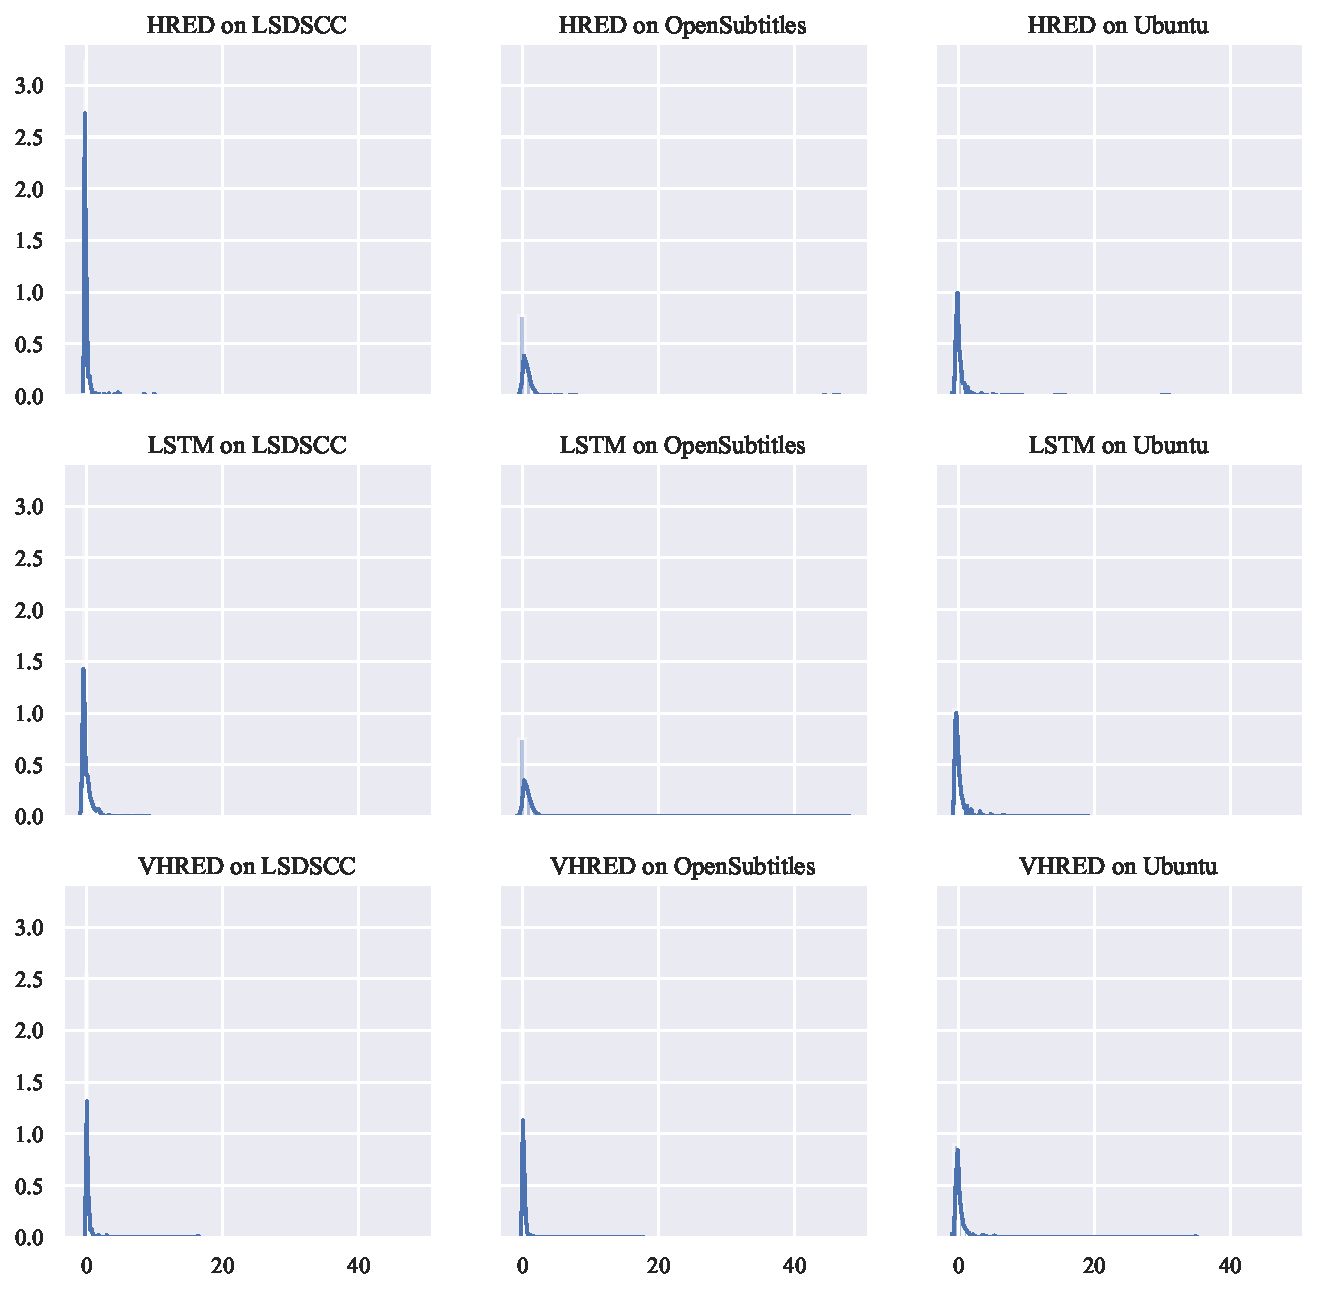
\includegraphics[width=\linewidth]{figure/distplot_grid/bleu_4/plot.pdf}
        \caption{BLEU-4}
    \end{subfigure}%
    \begin{subfigure}{0.33\linewidth}
        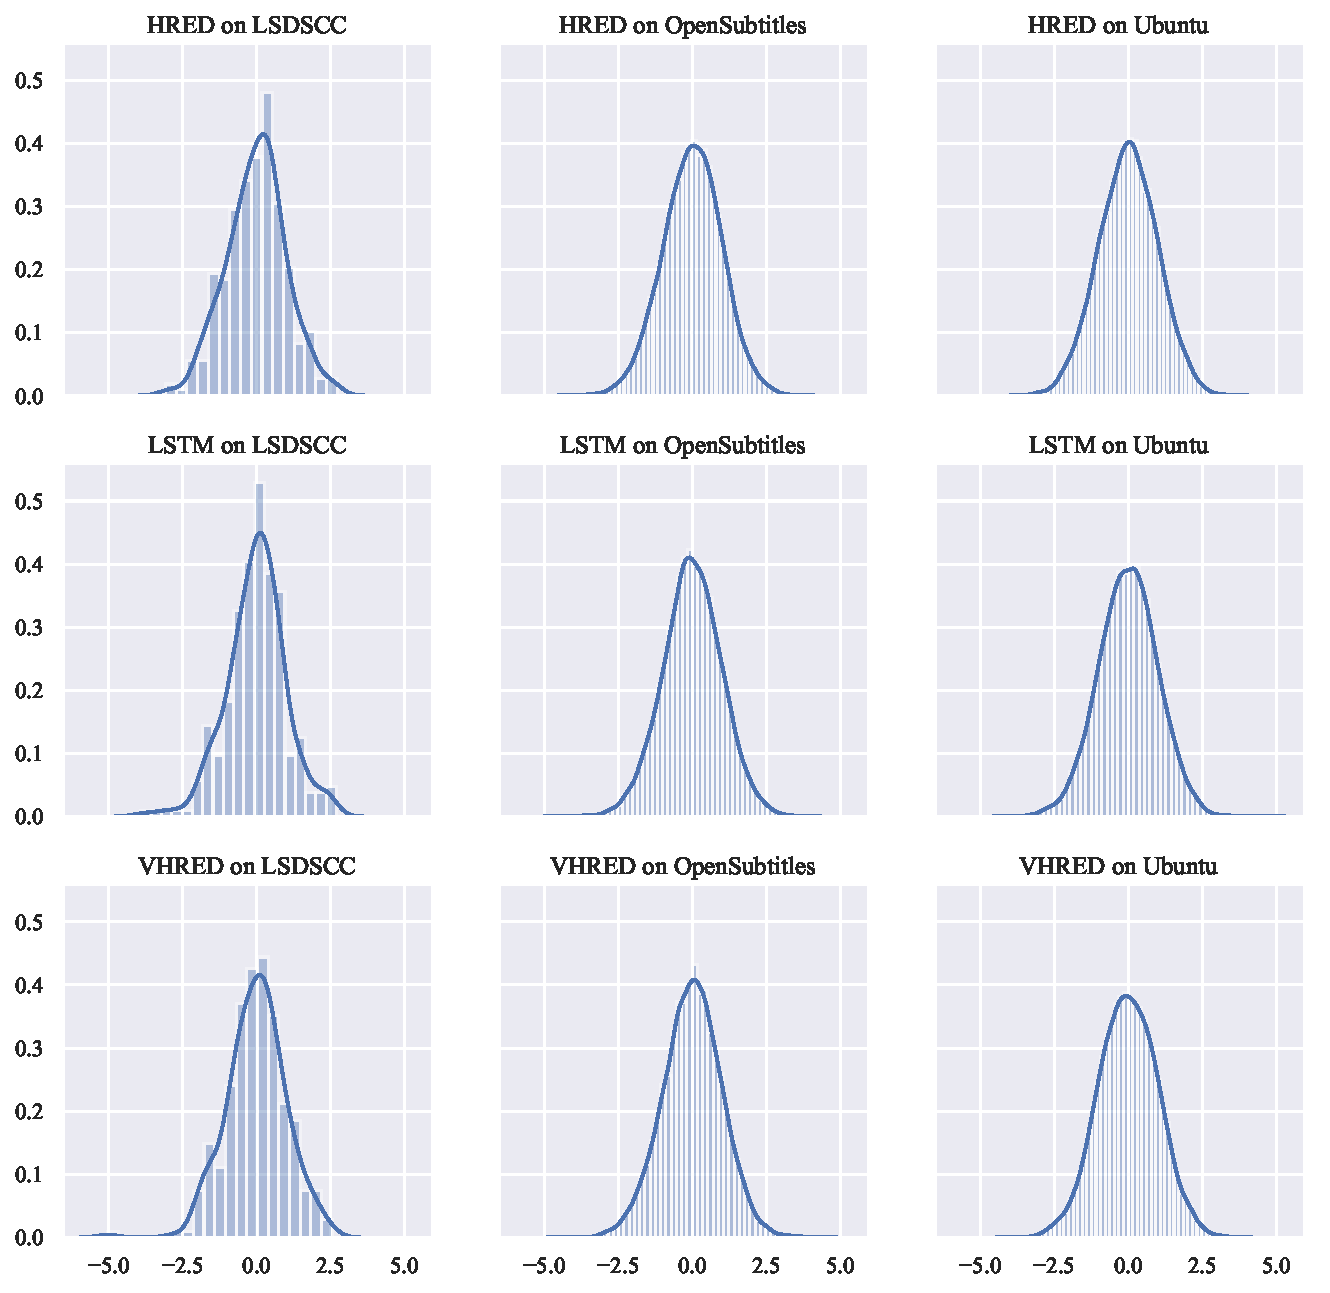
\includegraphics[width=\linewidth]{figure/distplot_grid/adem/plot.pdf}
        \centering
        \caption{ADEM}
    \end{subfigure}%
    \begin{subfigure}{0.33\linewidth}
        \centering
        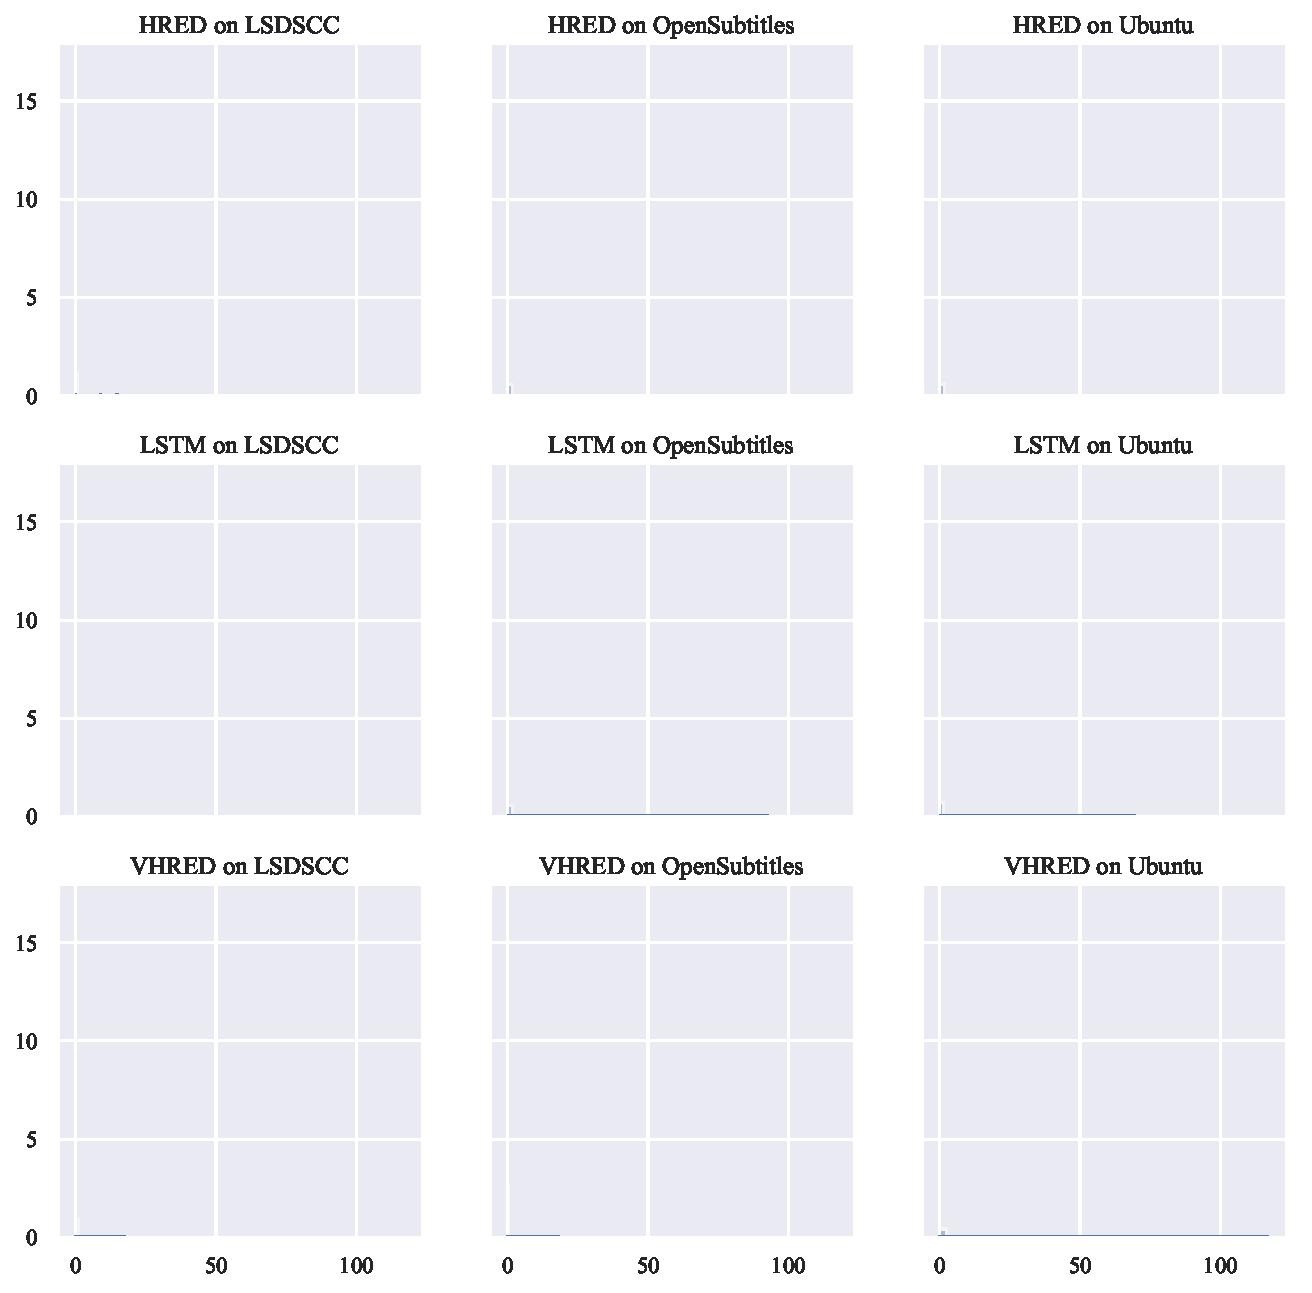
\includegraphics[width=\linewidth]{figure/distplot_grid/rouge_4/plot.pdf}
        \caption{ROUGE-4}
    \end{subfigure}
    \begin{subfigure}{0.33\linewidth}
        \centering
        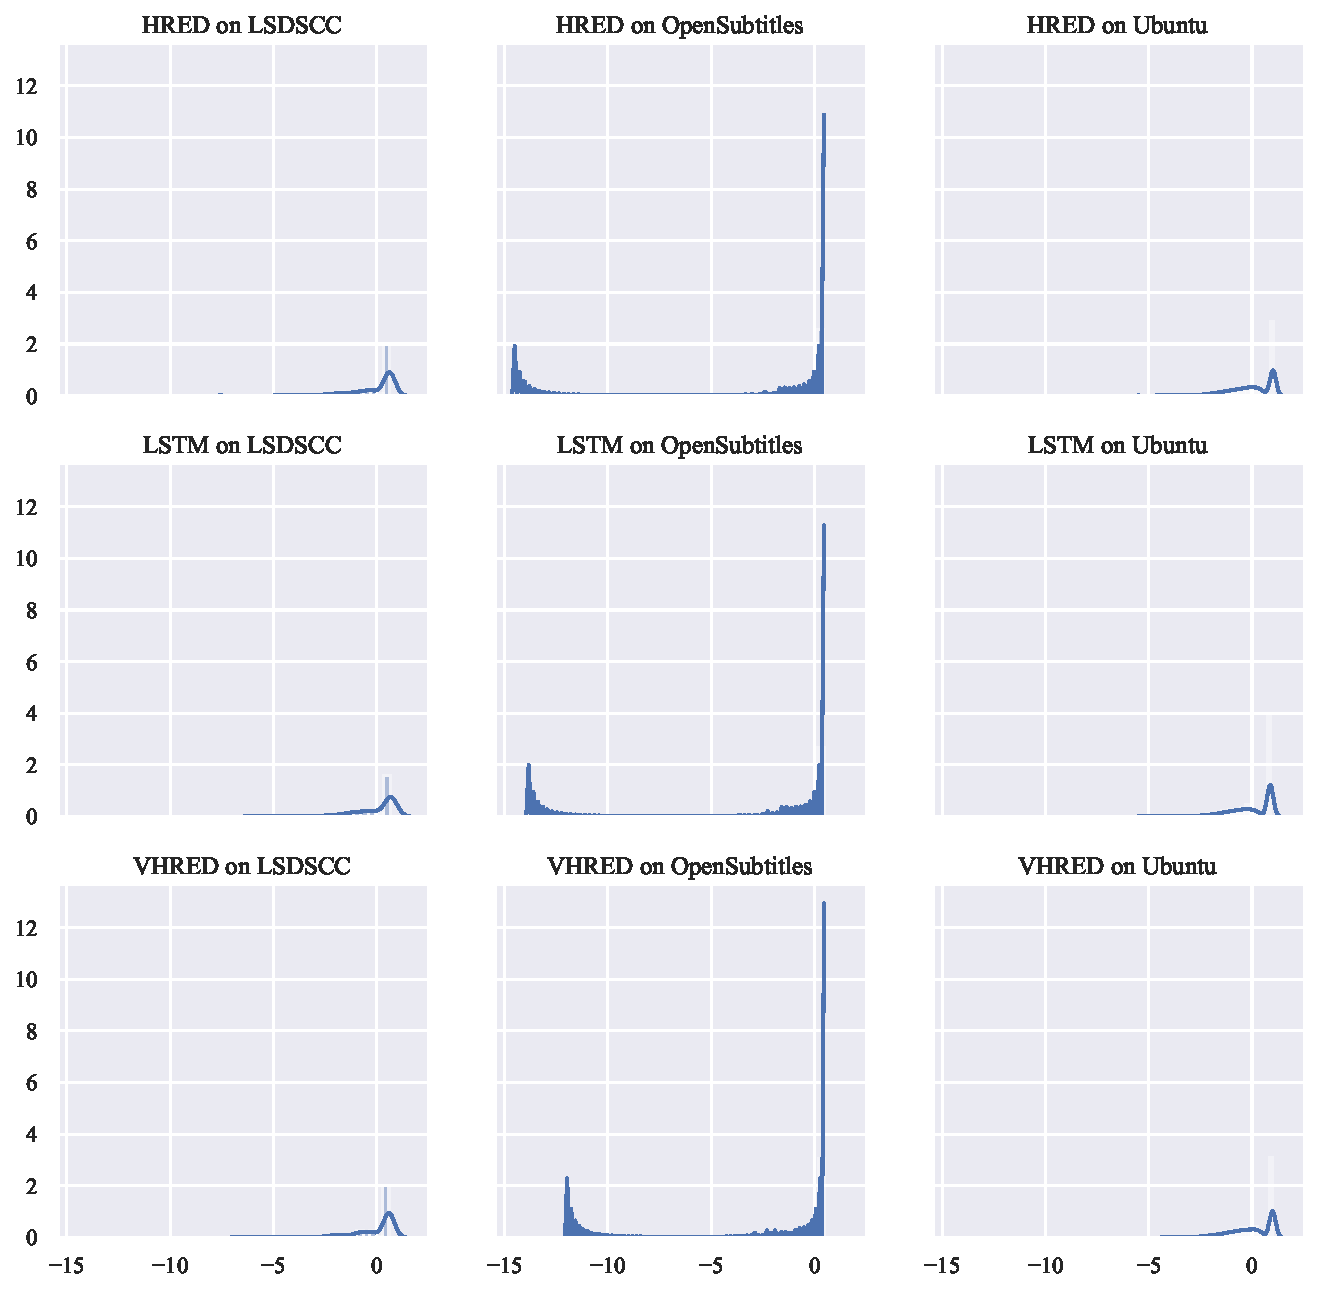
\includegraphics[width=\linewidth]{figure/distplot_grid/distinct_1/plot.pdf}
        \caption{Distinct-1}
    \end{subfigure}%
    \begin{subfigure}{0.33\linewidth}
        \centering
        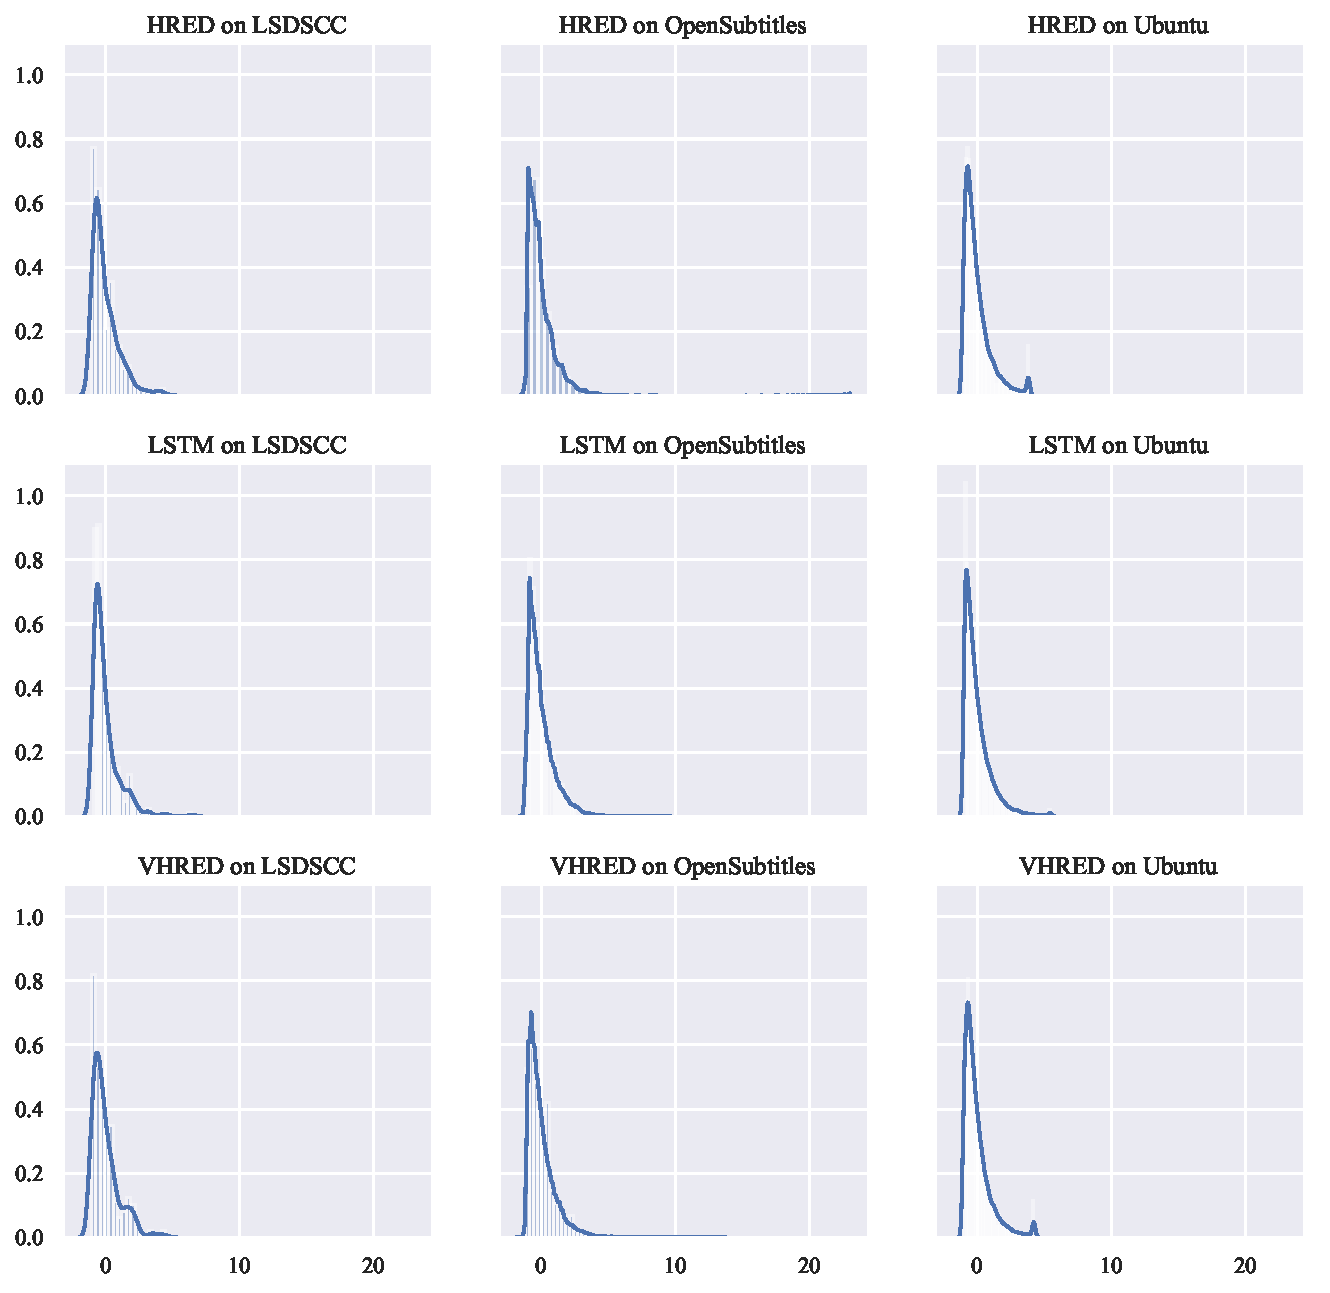
\includegraphics[width=\linewidth]{figure/distplot_grid/utterance_len/plot.pdf}
        \caption{\#words}
    \end{subfigure}%
    \begin{subfigure}{0.33\linewidth}
        \centering
        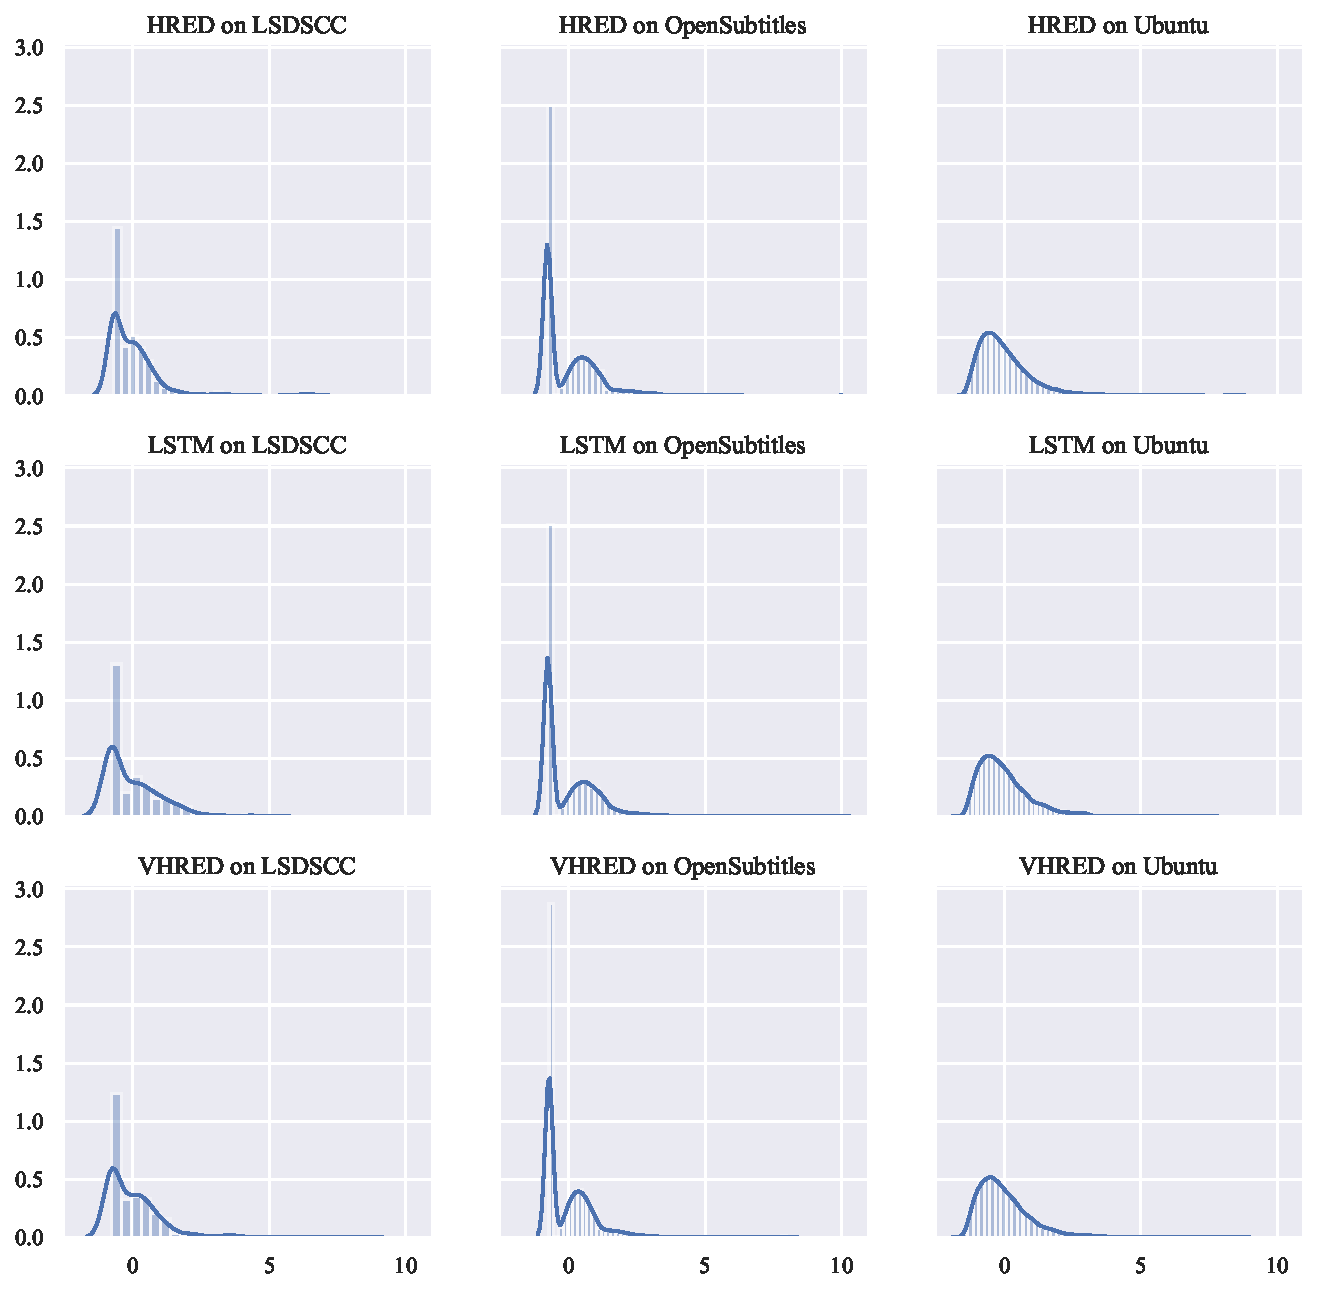
\includegraphics[width=\linewidth]{figure/distplot_grid/rouge_l/plot.pdf}
        \caption{ROUGE-L}
    \end{subfigure}
    \begin{subfigure}{0.33\linewidth}
        \centering
        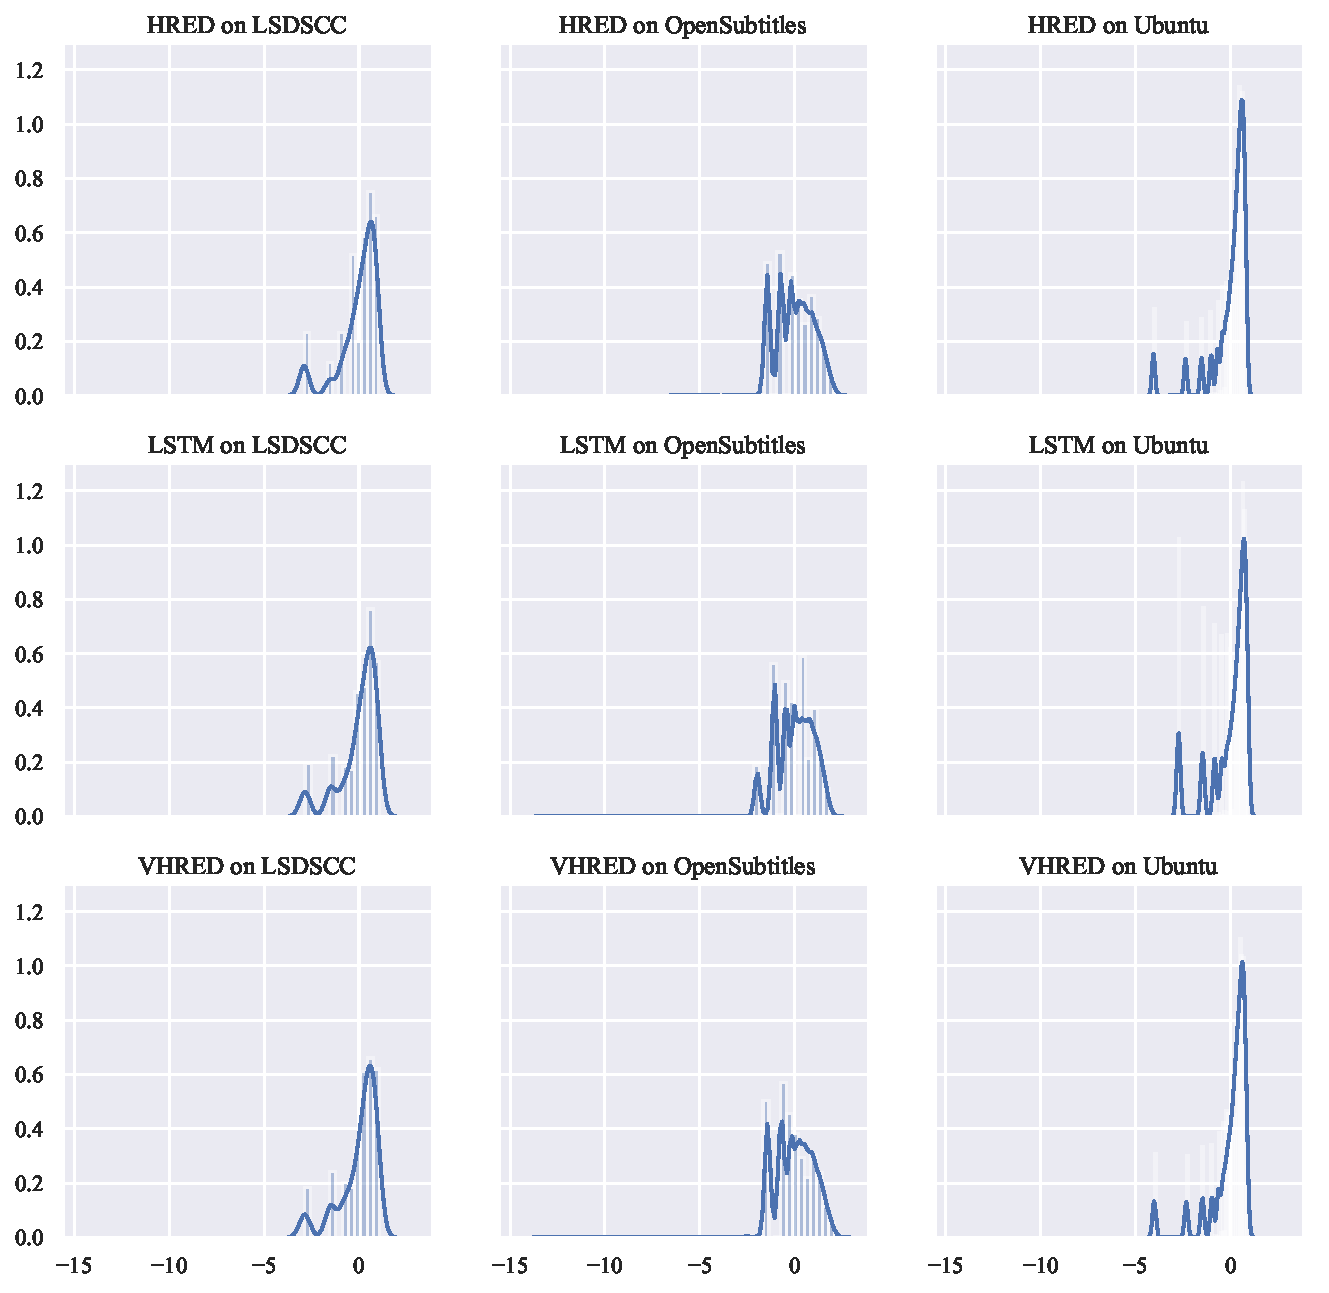
\includegraphics[width=\linewidth]{figure/distplot_grid/distinct_2/plot.pdf}
        \caption{Distinct-2}
    \end{subfigure}%
    \begin{subfigure}{0.33\linewidth}
        \centering
        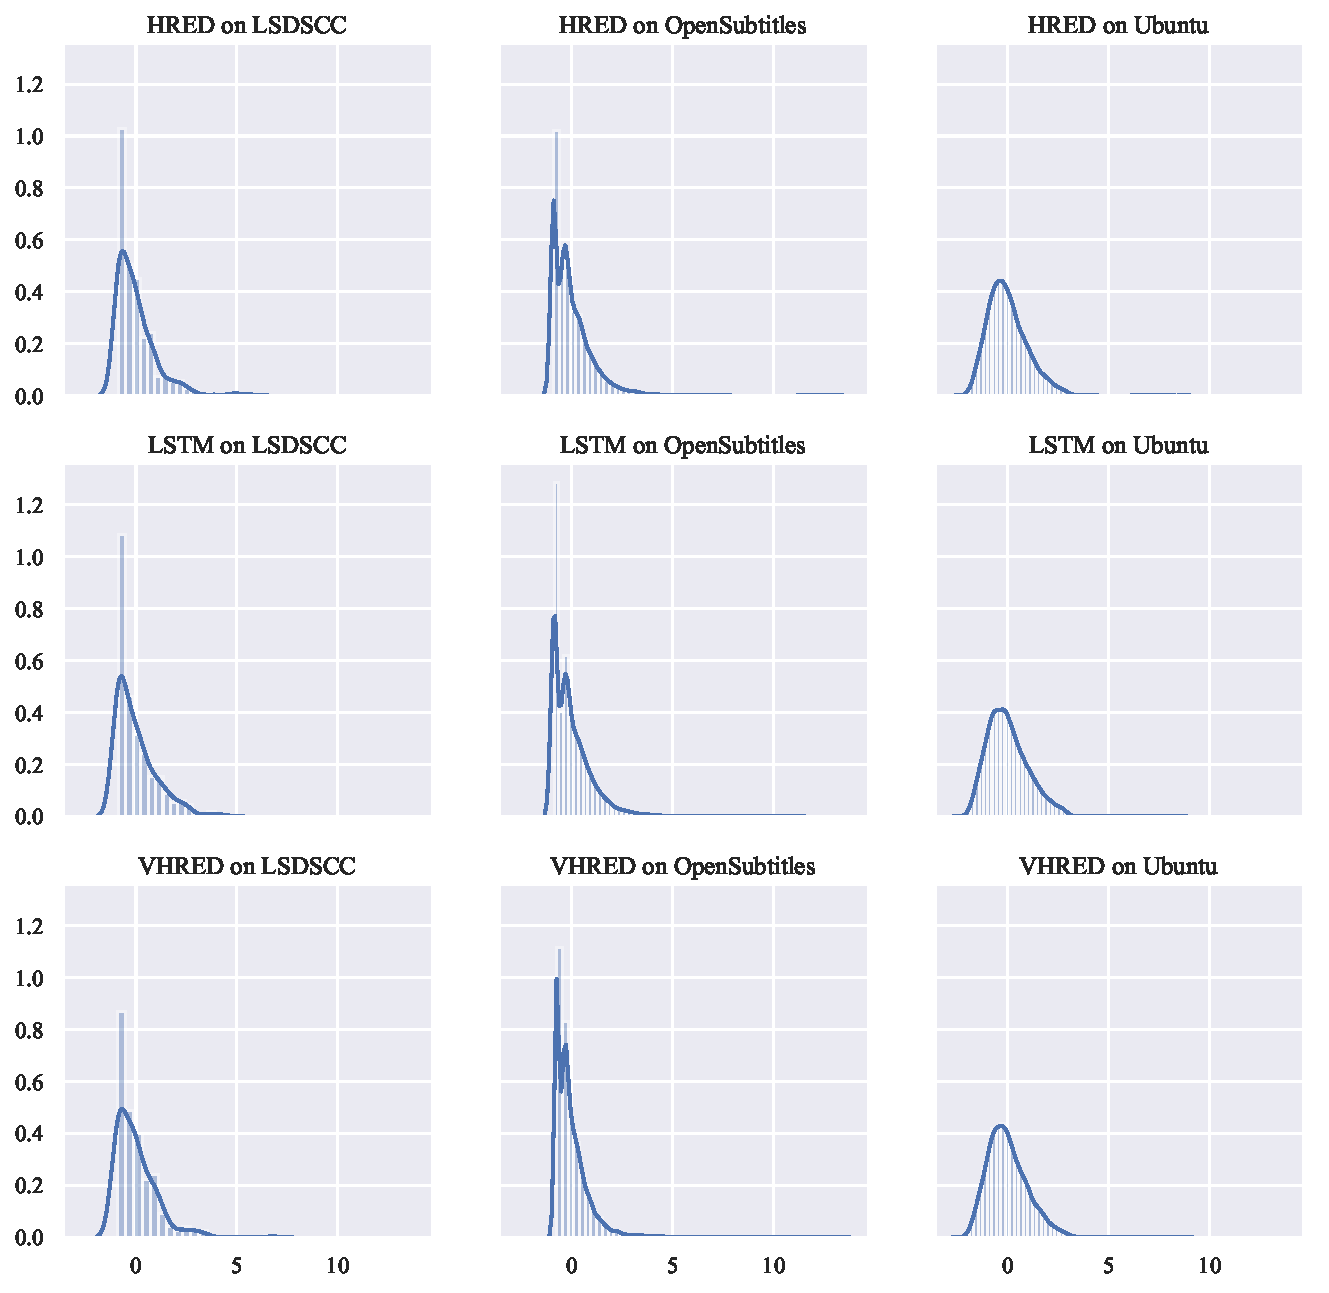
\includegraphics[width=\linewidth]{figure/distplot_grid/meteor/plot.pdf}
        \caption{METEOR}
    \end{subfigure}%
    \begin{subfigure}{0.33\linewidth}
        \centering
        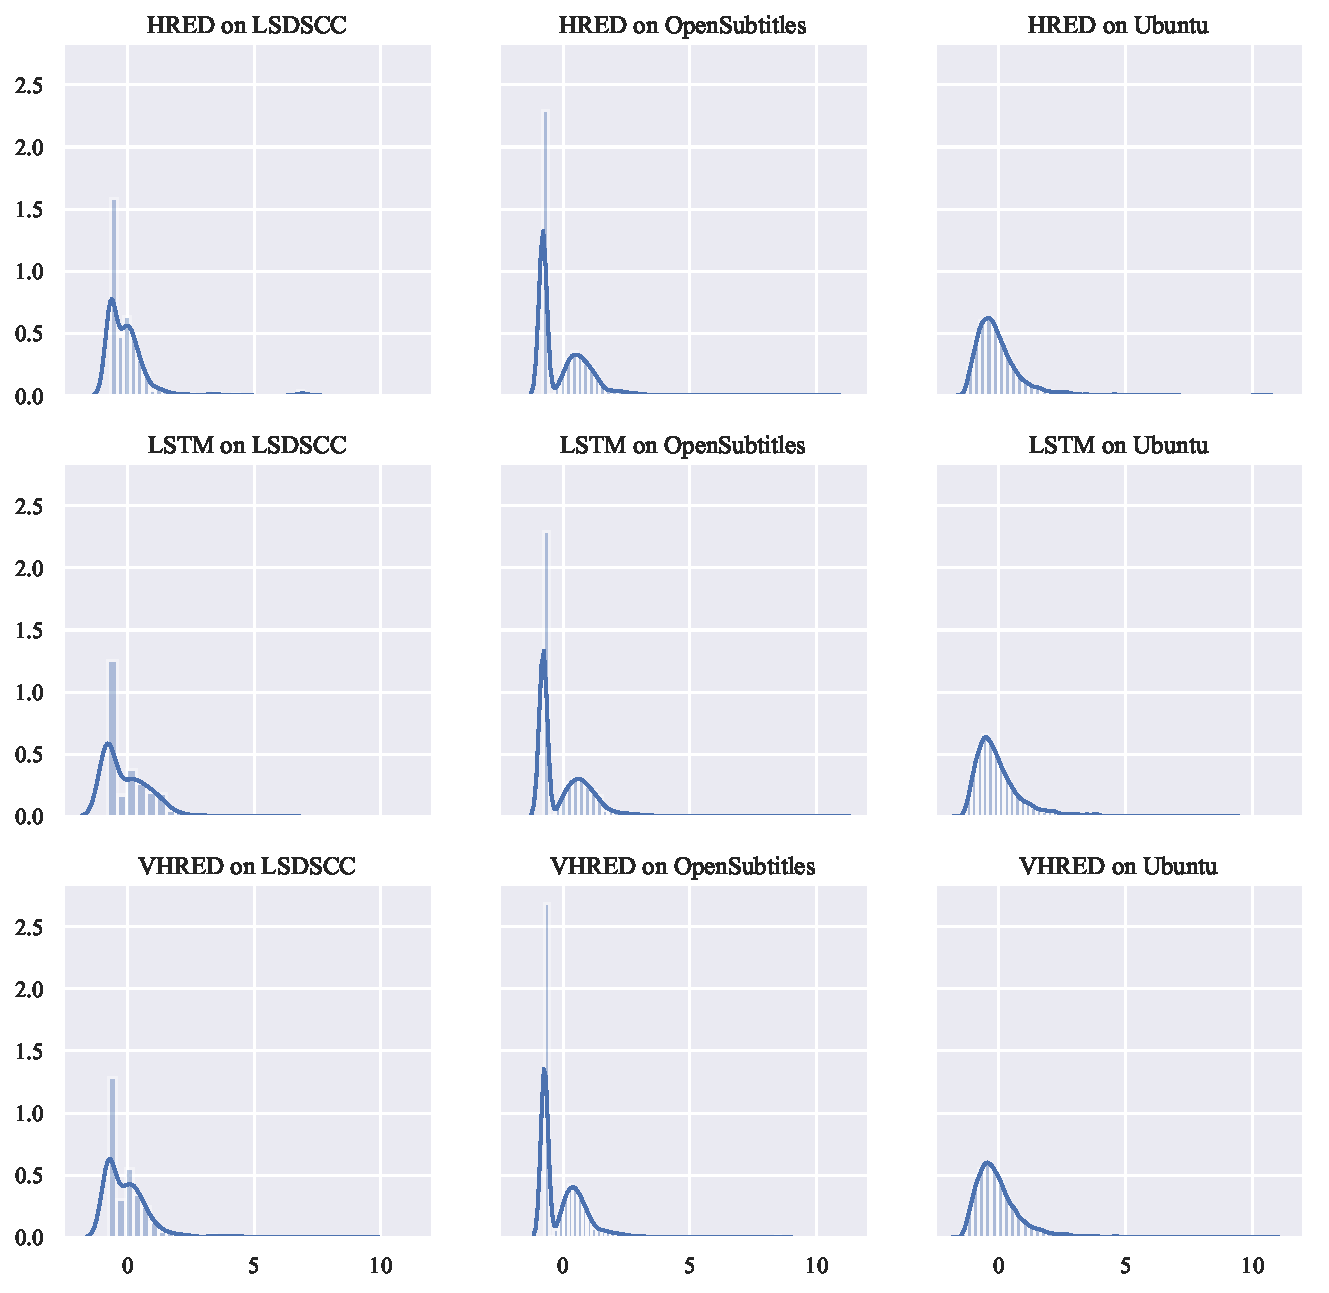
\includegraphics[width=\linewidth]{figure/distplot_grid/rouge_w/plot.pdf}
        \caption{ROUGE-W}
    \end{subfigure}
    \centering
    \caption{句子得分分布二}
\end{figure}

图~\ref{fig:ROUGE_system}~是ROUGE的系统得分柱形图。 从总体上看, 不同数据集上的模型在ROUGE-1,ROUGE-2,ROUGE-L和ROUGE-W的得分都不为0, 但在ROUGE-3和ROUGE-4上,多个模型的得分接近0, 这是正常的,因为一般来说,响应和参考之间的高阶n-gram重叠非常少。 ROUGE-1,ROUGE-L和ROUGE-W的图像非常相似。 在这三个指标上,在LSDSCC和OpenSubtitles上,HRED和VHRED超过了LSTM, 但在Ubuntu上,LSTM却超过了HRED和VHRED; 除此之外,各个数据集内三个模型的排名也基本一致, 但是模型之间的差距有时很大,比如LSDSCC上的ROUGE-2, 有时很小,比如OpenSubtitles上的ROUGE-1。

在ROUGE-3和ROUGE-4上,LSTM的得分在所有数据集上普遍很低, 而HRED和VHRED在某些数据集上得分也很低, 在Ubuntu上,所有模型的得分都很低。 令人注目的是,VHRED在OpenSubtitles和LSDSCC上都取得了不错的成绩, 而HRED的表现在LSDSCC上较好,在OpenSubtitles上较差。

% -- Other -- %
图~\ref{fig:Other_system}~是Distinct-N, METEOR和句子长度的系统得分图。 在Ubuntu上的模型的句子长度明显大于 在LSDSCC上的模型,而后者大于在OpenSubtitles上的模型。 第~\ref{sec:dataset_proprecessing}~节表明, 各数据集在训练集的平均句子长度上的关系是:Ubuntu大于LSDSCC大于OpenSubtitles。 模型生成的响应的长度和训练集的平均句子长度具有一致性, 这是因为训练的目标函数是最大化训练集样本的对数概率, 所以模型倾向于模仿训练集的统计特征。

Distinct-N对模型的区分度不高, 在同一个数据集上训练的模型,它们的Distinct-N都比较接近。 从数据集的角度,OpenSubtitles上的模型的Distinct-1较高, 而Ubuntu上的模型的Distinct-2较高。 METEOR似乎受句子长度的影响较大, 在句子长度较大的Ubuntu上,模型的METEOR得分要比其他数据集上的得分高得多。 而LSDSCC上的METEOR也比OpenSubtitles上的得分略高。 METEOR对不同模型的区分度不是很大, 但从总体上看,HRED和VHRED比LSTM的表现要好。
% MIT License
% 
% Copyright (c) 2019 Cong Feng
% 
% Permission is hereby granted, free of charge, to any person obtaining a copy
% of this software and associated documentation files (the "Software"), to deal
% in the Software without restriction, including without limitation the rights
% to use, copy, modify, merge, publish, distribute, sublicense, and/or sell
% copies of the Software, and to permit persons to whom the Software is
% furnished to do so, subject to the following conditions:
% 
% The above copyright notice and this permission notice shall be included in all
% copies or substantial portions of the Software.
% 
% THE SOFTWARE IS PROVIDED "AS IS", WITHOUT WARRANTY OF ANY KIND, EXPRESS OR
% IMPLIED, INCLUDING BUT NOT LIMITED TO THE WARRANTIES OF MERCHANTABILITY,
% FITNESS FOR A PARTICULAR PURPOSE AND NONINFRINGEMENT. IN NO EVENT SHALL THE
% AUTHORS OR COPYRIGHT HOLDERS BE LIABLE FOR ANY CLAIM, DAMAGES OR OTHER
% LIABILITY, WHETHER IN AN ACTION OF CONTRACT, TORT OR OTHERWISE, ARISING FROM,
% OUT OF OR IN CONNECTION WITH THE SOFTWARE OR THE USE OR OTHER DEALINGS IN THE
% SOFTWARE.

\begin{figure}[H]
    \begin{subfigure}{0.4\linewidth}
        \centering
        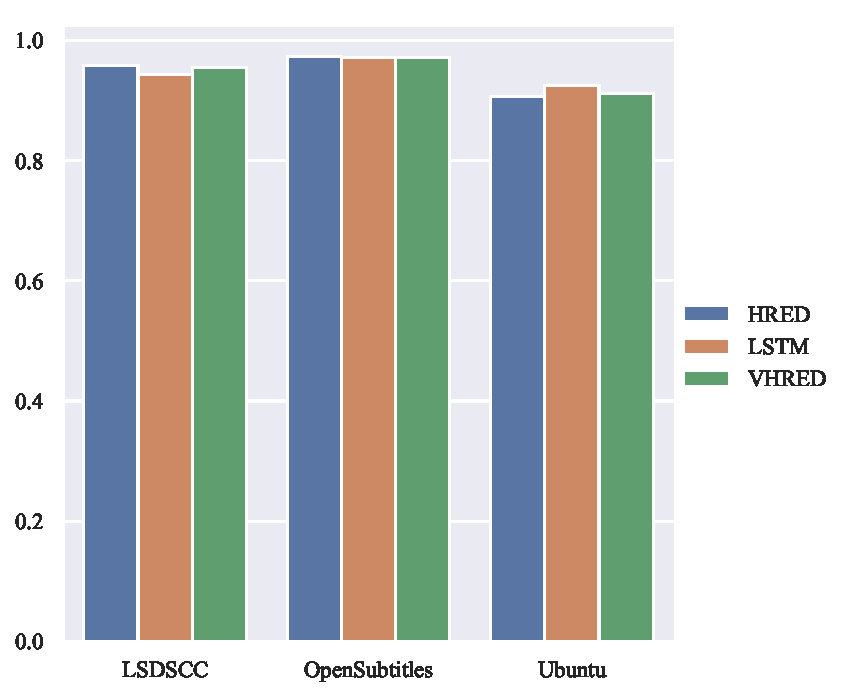
\includegraphics[width=\linewidth]{figure/barplot/distinct_1/plot.pdf}
        \caption{Distinct-1}
        \label{fig:distinct_1_system}
    \end{subfigure}%
    \begin{subfigure}{0.4\linewidth}
        \centering
        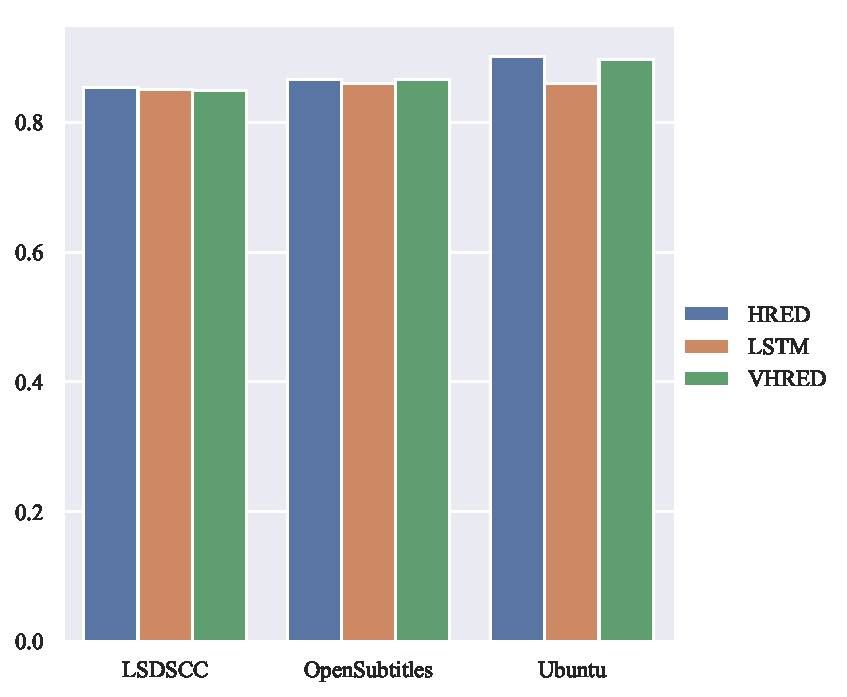
\includegraphics[width=\linewidth]{figure/barplot/distinct_2/plot.pdf}
        \caption{Distinct-2}
        \label{fig:distinct_2_system}
    \end{subfigure}
    \begin{subfigure}{0.4\linewidth}
        \centering
        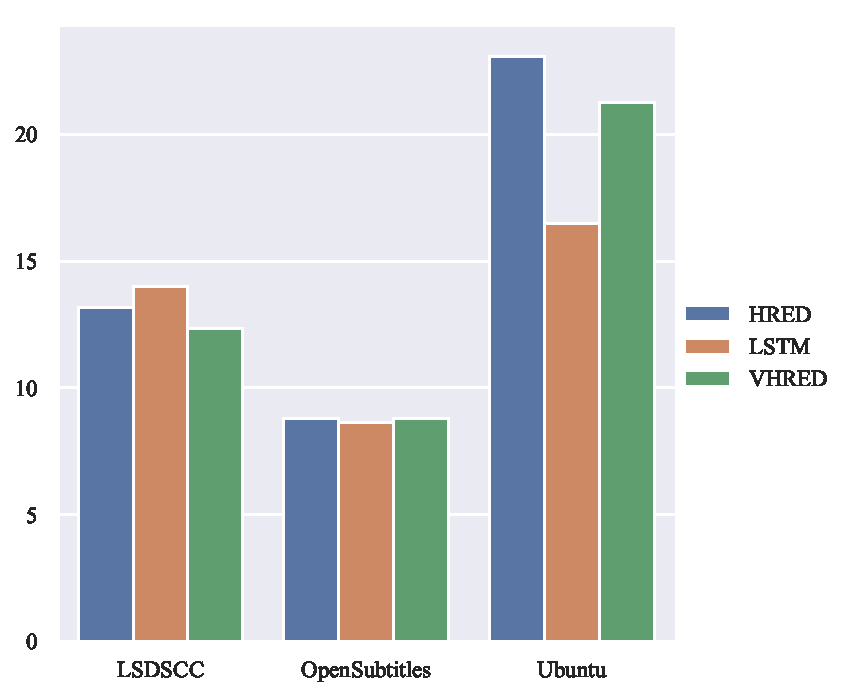
\includegraphics[width=\linewidth]{figure/barplot/utterance_len/plot.pdf}
        \caption{\#words}
        \label{fig:words_system}
    \end{subfigure}%
    \begin{subfigure}{0.4\linewidth}
        \centering
        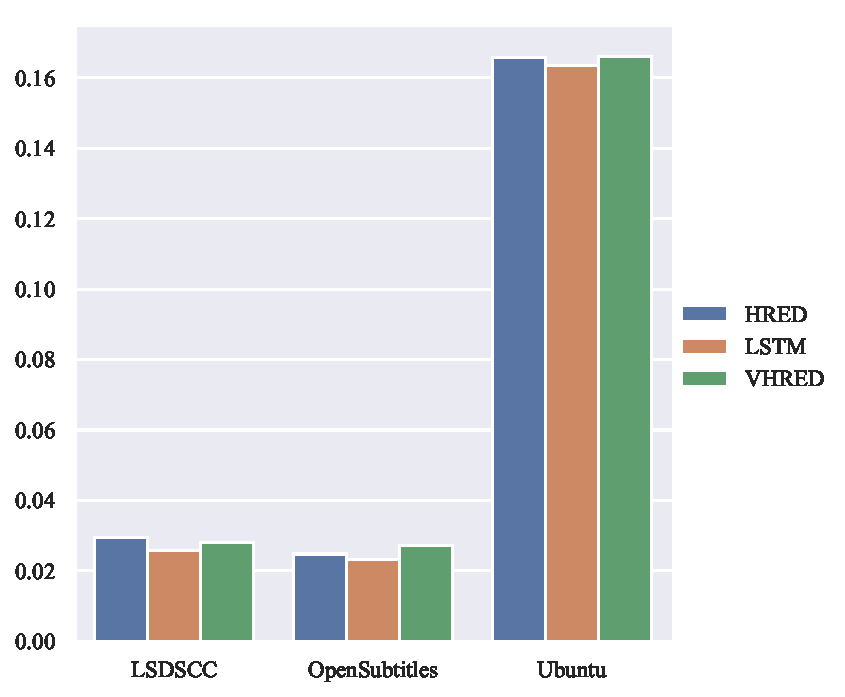
\includegraphics[width=\linewidth]{figure/barplot/meteor/plot.pdf}
        \caption{METEOR}
        \label{fig:meteor_system}
    \end{subfigure}
    \centering
    \caption{Distinct-N,\#words和METEOR的系统得分}
    \label{fig:Other_system}
\end{figure}


% -- Conclusion -- %
本节利用柱状图分析了模型,数据集和指标的系统层面得分。 在一些图中,各个模型的得分差异不是十分明显, 为了突显得分的差异,本文把观察的维度分成数据集和模型两个维度, 并分别绘制了箱体图。 通过箱体图得出的结论是相同的,但是由于图像的数量较多,所以放在了附录。 附录~\ref{ch:dataset_system_dist}~从 数据集的维度和模型的维度展示了不同指标的系统层面得分。

% --------------------- %
% -- Utterance Level -- %
% --------------------- %
\section{句子层面得分}\label{sec:utterance_scores}
本文还从句子层面得分方面进行了分析。 因为模型生成的句子$u$可以看做句子空间$U$上的随机变量, 而指标是一个确定的函数$f_{s}$, 可以把句子层面的得分看做一个随机变量$\lambda_u = f_{s}(u)$, 于是可以用描述统计学(Descriptive Statistics)和统计推断(Statistical Inference) 的方法来分析指标在句子水平的情况。

本文绘制了各种指标的句子层面得分的单变量分布(Univariate Distribution)。 为了便于从图像上比较各种指标的分布特征,本文对数据作了归一化处理, 使数据的平均值为0,标准差为1:
\begin{align}
    x' = \frac{x - \mu}{\sigma}
\end{align}
$\mu$是$x$的平均值,$\sigma$是$x$的标准差,$x'$是归一化之后的数据。 为了使读者能快速检阅所有指标的分布情况, 本文对所有模型和数据集的组合采用了案例分析(Case Study)的方法, 详细分析了模型为HRED,数据集为OpenSubtitles的各项指标的分布。 附录~\ref{ch:metric_dist}~展示了所有的组合上的指标分布。

% -- BLEU -- %
\begin{figure}[H]
    \begin{subfigure}{0.4\linewidth}
        \centering
        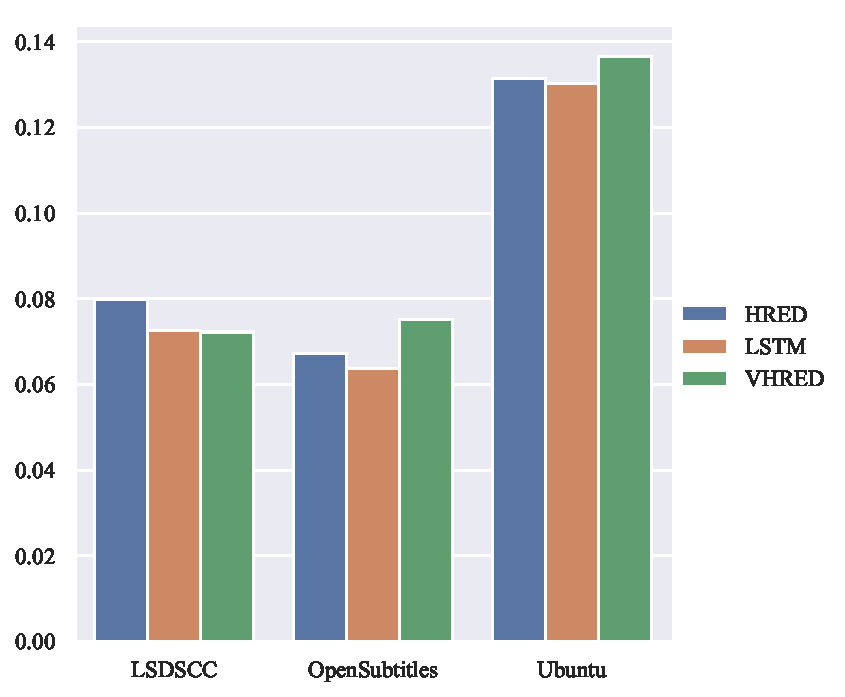
\includegraphics[width=\linewidth]{figure/barplot/bleu_1/plot.pdf}
        \caption{BLEU-1}
    \end{subfigure}%
    \begin{subfigure}{0.4\linewidth}
        \centering
        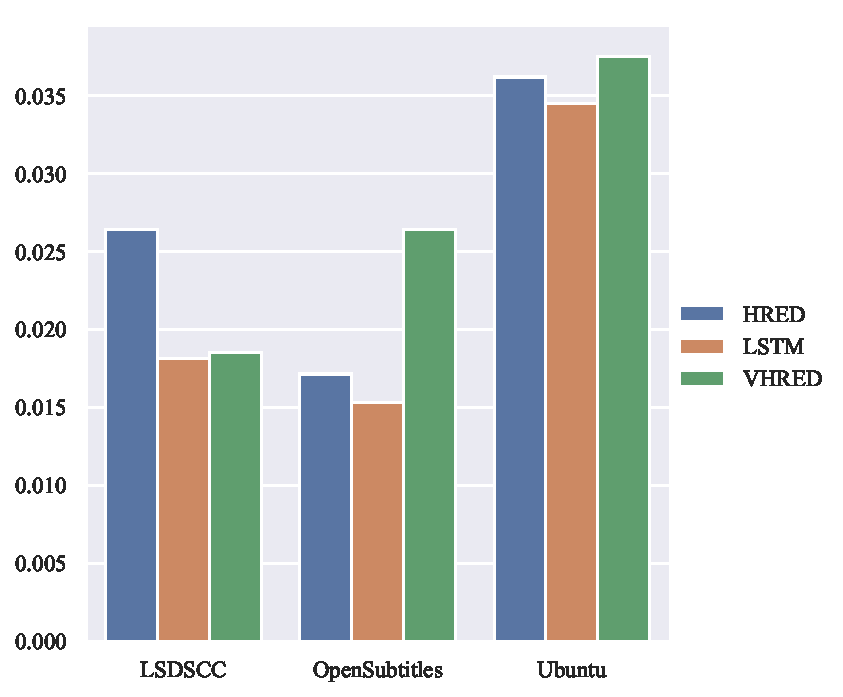
\includegraphics[width=\linewidth]{figure/barplot/bleu_2/plot.pdf}
        \caption{BLEU-2}
    \end{subfigure}
    \begin{subfigure}{0.4\linewidth}
        \centering
        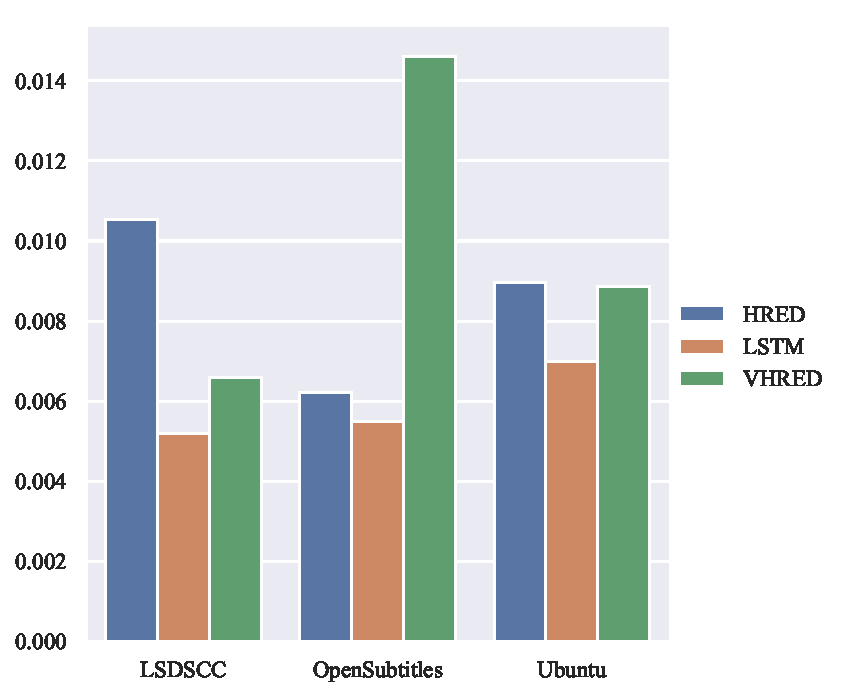
\includegraphics[width=\linewidth]{figure/barplot/bleu_3/plot.pdf}
        \caption{BLEU-3}
    \end{subfigure}%
    \begin{subfigure}{0.4\linewidth}
        \centering
        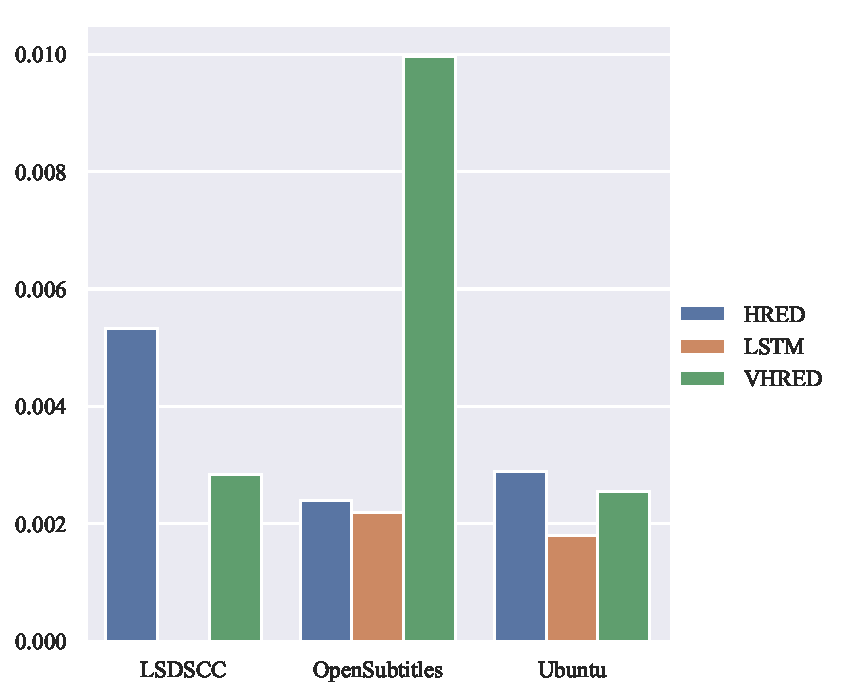
\includegraphics[width=\linewidth]{figure/barplot/bleu_4/plot.pdf}
        \caption{BLEU-4}
    \end{subfigure}
    \centering
    \caption{BLEU的系统得分}
    \label{fig:BLEU_system}
\end{figure}

图~\ref{fig:BLEU_dist}~是BLEU的N取1到4时的分布图。
由于加入了平滑处理,所以大部分得分都有非零数值,
在均值附近集中了大量的句子,
这可能是因为大部分句子的得分非常低\upcite{HowNot}。
一元词匹配相对高阶n-gram匹配更容易,
所以BLEU-1在均值的右边有一个低矮的峰值,
并且峰值对应的横坐标偏离了均值0,
这说明有相当一部分句子的得分高于均值。
而低于均值的部分出现了一个高峰,说明也有大量句子得分低于均值。
BLEU-2至4的分布都非常相似,
只是峰值的横坐标比BLEU-1更接近均值。
从总体上来说,BLEU的分布形状十分尖锐,大量句子集中在均值附近,
图像不对称, 峰值比高斯分布的峰值$1 / \sqrt{2 \pi} \approx 0.4$高。

% -- ADEM_AND_EB -- %
% MIT License
% 
% Copyright (c) 2019 Cong Feng
% 
% Permission is hereby granted, free of charge, to any person obtaining a copy
% of this software and associated documentation files (the "Software"), to deal
% in the Software without restriction, including without limitation the rights
% to use, copy, modify, merge, publish, distribute, sublicense, and/or sell
% copies of the Software, and to permit persons to whom the Software is
% furnished to do so, subject to the following conditions:
% 
% The above copyright notice and this permission notice shall be included in all
% copies or substantial portions of the Software.
% 
% THE SOFTWARE IS PROVIDED "AS IS", WITHOUT WARRANTY OF ANY KIND, EXPRESS OR
% IMPLIED, INCLUDING BUT NOT LIMITED TO THE WARRANTIES OF MERCHANTABILITY,
% FITNESS FOR A PARTICULAR PURPOSE AND NONINFRINGEMENT. IN NO EVENT SHALL THE
% AUTHORS OR COPYRIGHT HOLDERS BE LIABLE FOR ANY CLAIM, DAMAGES OR OTHER
% LIABILITY, WHETHER IN AN ACTION OF CONTRACT, TORT OR OTHERWISE, ARISING FROM,
% OUT OF OR IN CONNECTION WITH THE SOFTWARE OR THE USE OR OTHER DEALINGS IN THE
% SOFTWARE.

\begin{figure}[H]
    \begin{subfigure}{0.45\linewidth}
        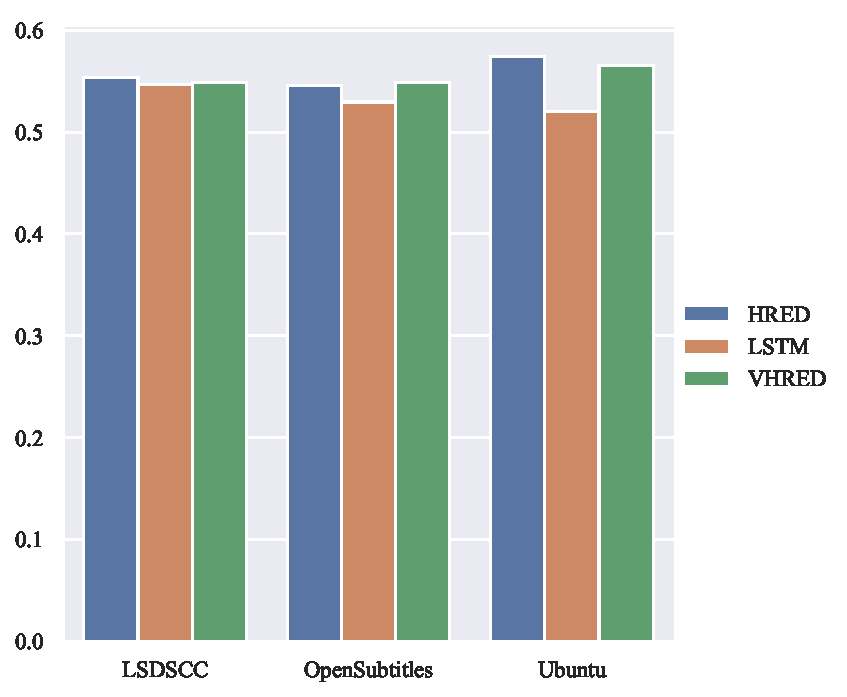
\includegraphics[width=\linewidth]{figure/barplot/embedding_based_vector_average/plot.pdf}
        \centering
        \caption{Average}
    \end{subfigure}%
    \begin{subfigure}{0.45\linewidth}
        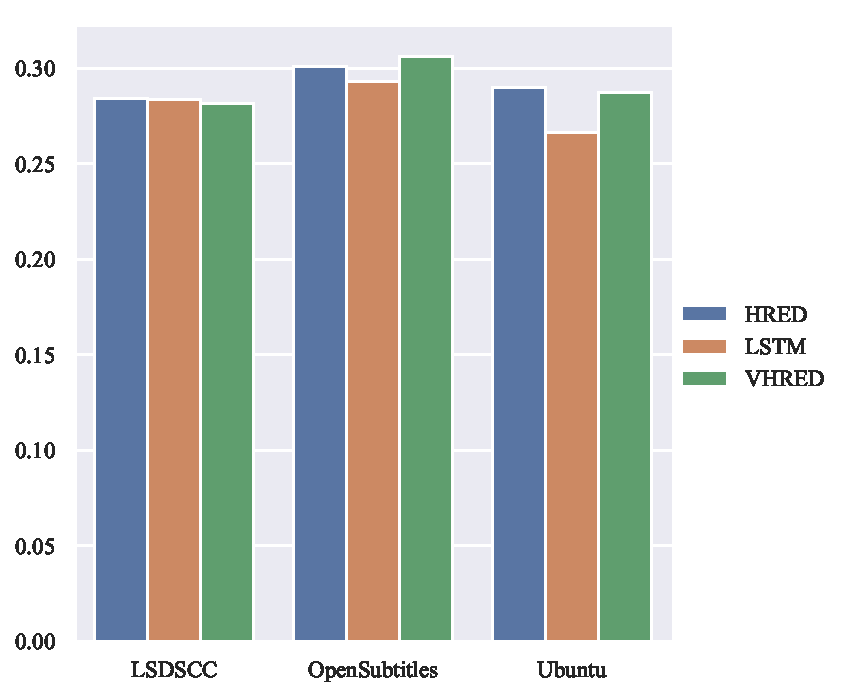
\includegraphics[width=\linewidth]{figure/barplot/embedding_based_vector_extrema/plot.pdf}
        \centering
        \caption{Extrema}
    \end{subfigure}
    \begin{subfigure}{0.45\linewidth}
        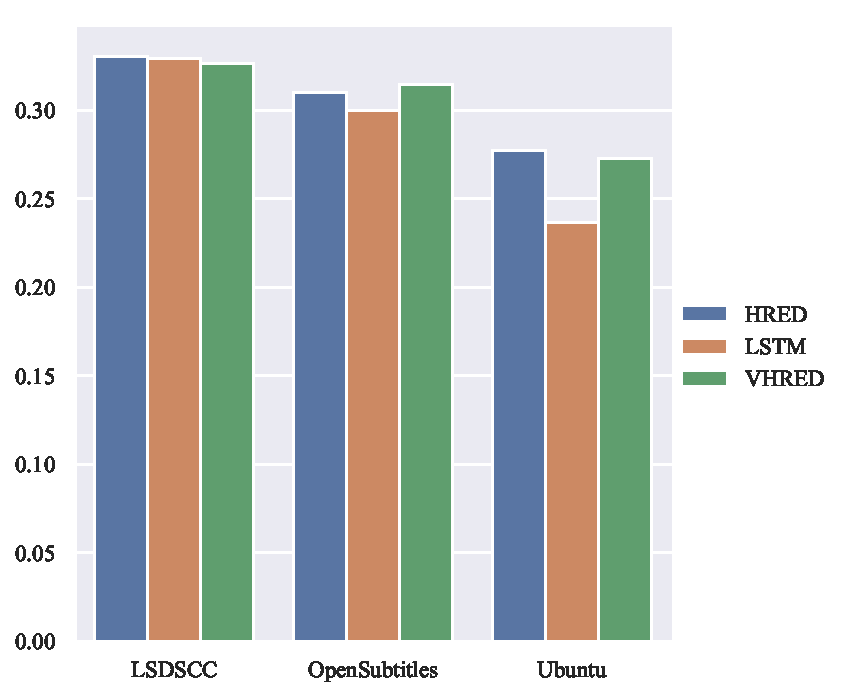
\includegraphics[width=\linewidth]{figure/barplot/embedding_based_greedy_matching/plot.pdf}
        \centering
        \caption{Greedy}
    \end{subfigure}%
    \begin{subfigure}{0.45\linewidth}
        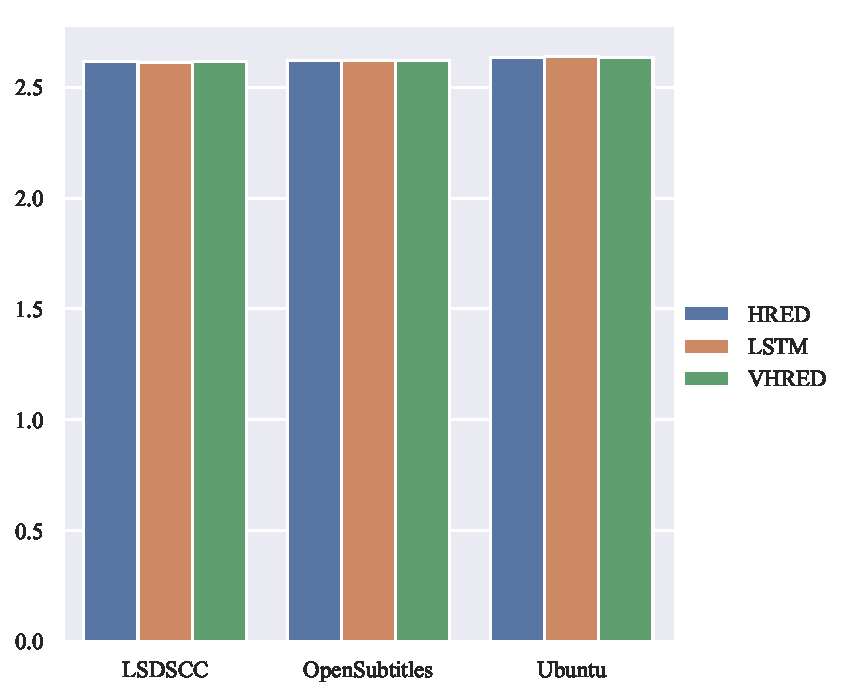
\includegraphics[width=\linewidth]{figure/barplot/adem/plot.pdf}
        \centering
        \caption{ADEM}
        \label{subfig:ADEM_system}
    \end{subfigure}
    \centering
    \caption{基于词嵌入的指标和ADEM的系统得分}
    \label{fig:ADEM_EB_system}
\end{figure}

图~\ref{fig:ADEM_EB_dist}~是基于词嵌入的指标和ADEM指标的分布图。 因为ADEM可以看做是一种更高级的词嵌入指标,所以把它和其他词嵌入指标并列。 四个图像均呈钟型曲线,峰值非常接近0.4,峰值的横坐标则非常接近0。 ADEM曲线显示出几乎完美的对称,Greedy曲线的对称度次之, Average曲线向右边偏移,Extrema曲线向左边偏移。 ADEM和词嵌入指标有相似之处。 从句子向量的组合方式来看, Average的组合方法是平均值,Extrema的组合方法是极端值, 而ADEM的组合方法是预训练的VHRED编码器。 与其他词嵌入指标不同的是,ADEM考虑了上下文的影响, 使用神经网络对上下文,响应和参考三者加权, 并且显式的优化了和人类评价的相关性, 可见其采用的机制比一般的基于词嵌入的指标更加复杂。 Lowe在文献\cite{ADEM}中指出,ADEM倾向于保守打分, 即人类评价给高分的句子,ADEM倾向于给稍低的分数。 从ADEM的分布曲线上可以验证这一点: 得分高于平均值的句子与得分低于平均值的句子几乎一样多, 说明它不倾向于打高分或者低分。 值得注意的是,这些指标的分布非常接近高斯分布, 本文尚不清楚背后的原理是什么。 解释这些指标的分布接近高斯分布的原因将会是后续工作的一个方面。

% -- ROUGE -- %
% MIT License
% 
% Copyright (c) 2022 cgsdfc
% 
% Permission is hereby granted, free of charge, to any person obtaining a copy
% of this software and associated documentation files (the "Software"), to deal
% in the Software without restriction, including without limitation the rights
% to use, copy, modify, merge, publish, distribute, sublicense, and/or sell
% copies of the Software, and to permit persons to whom the Software is
% furnished to do so, subject to the following conditions:
% 
% The above copyright notice and this permission notice shall be included in all
% copies or substantial portions of the Software.
% 
% THE SOFTWARE IS PROVIDED "AS IS", WITHOUT WARRANTY OF ANY KIND, EXPRESS OR
% IMPLIED, INCLUDING BUT NOT LIMITED TO THE WARRANTIES OF MERCHANTABILITY,
% FITNESS FOR A PARTICULAR PURPOSE AND NONINFRINGEMENT. IN NO EVENT SHALL THE
% AUTHORS OR COPYRIGHT HOLDERS BE LIABLE FOR ANY CLAIM, DAMAGES OR OTHER
% LIABILITY, WHETHER IN AN ACTION OF CONTRACT, TORT OR OTHERWISE, ARISING FROM,
% OUT OF OR IN CONNECTION WITH THE SOFTWARE OR THE USE OR OTHER DEALINGS IN THE
% SOFTWARE.

\begin{figure}[H]
    \begin{subfigure}{0.33\linewidth}
        \centering
        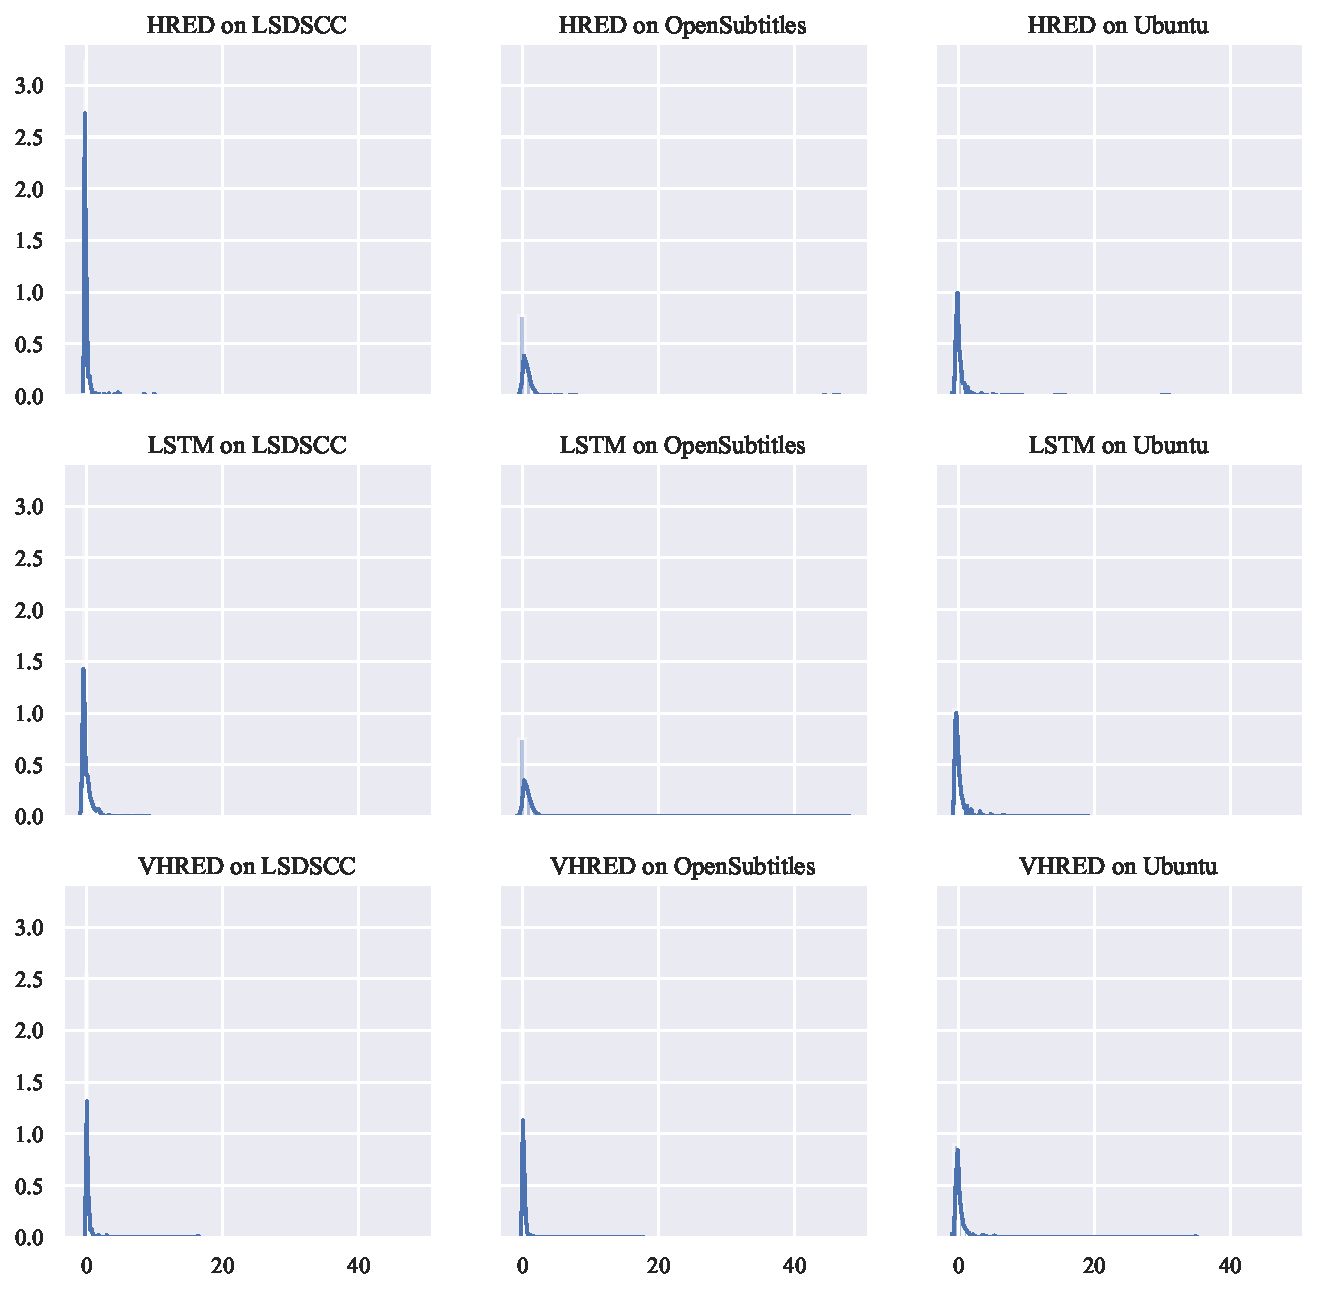
\includegraphics[width=\linewidth]{figure/distplot_grid/bleu_4/plot.pdf}
        \caption{BLEU-4}
    \end{subfigure}%
    \begin{subfigure}{0.33\linewidth}
        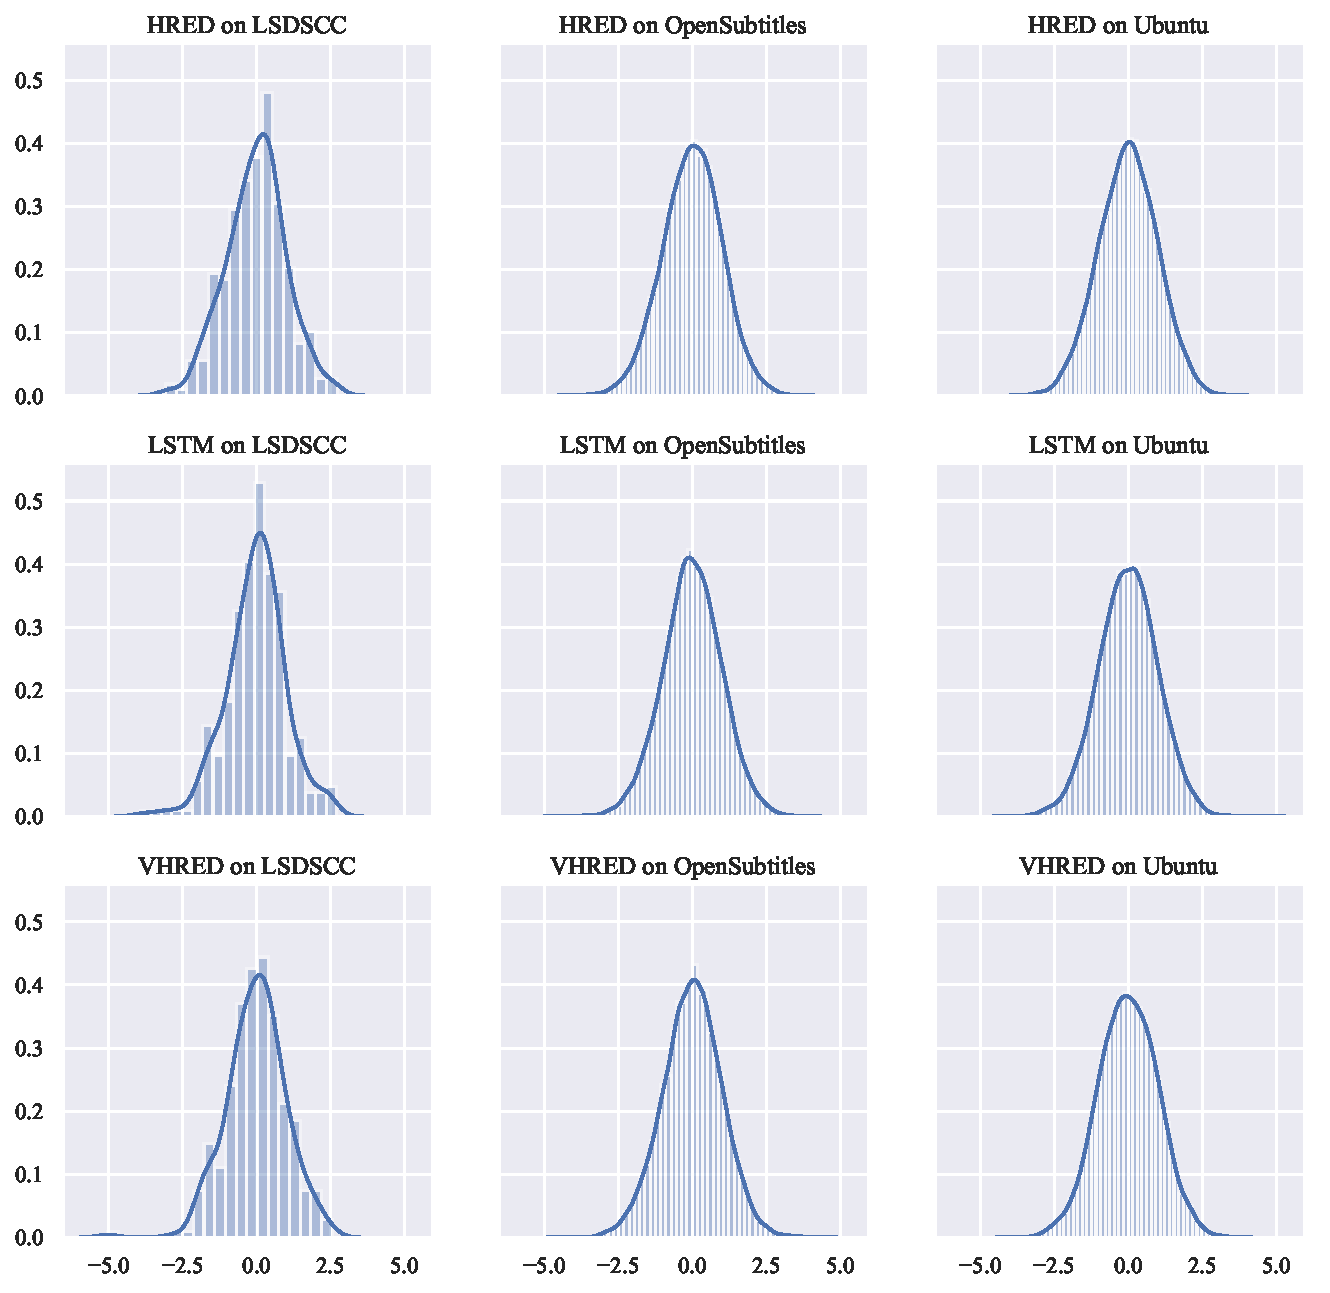
\includegraphics[width=\linewidth]{figure/distplot_grid/adem/plot.pdf}
        \centering
        \caption{ADEM}
    \end{subfigure}%
    \begin{subfigure}{0.33\linewidth}
        \centering
        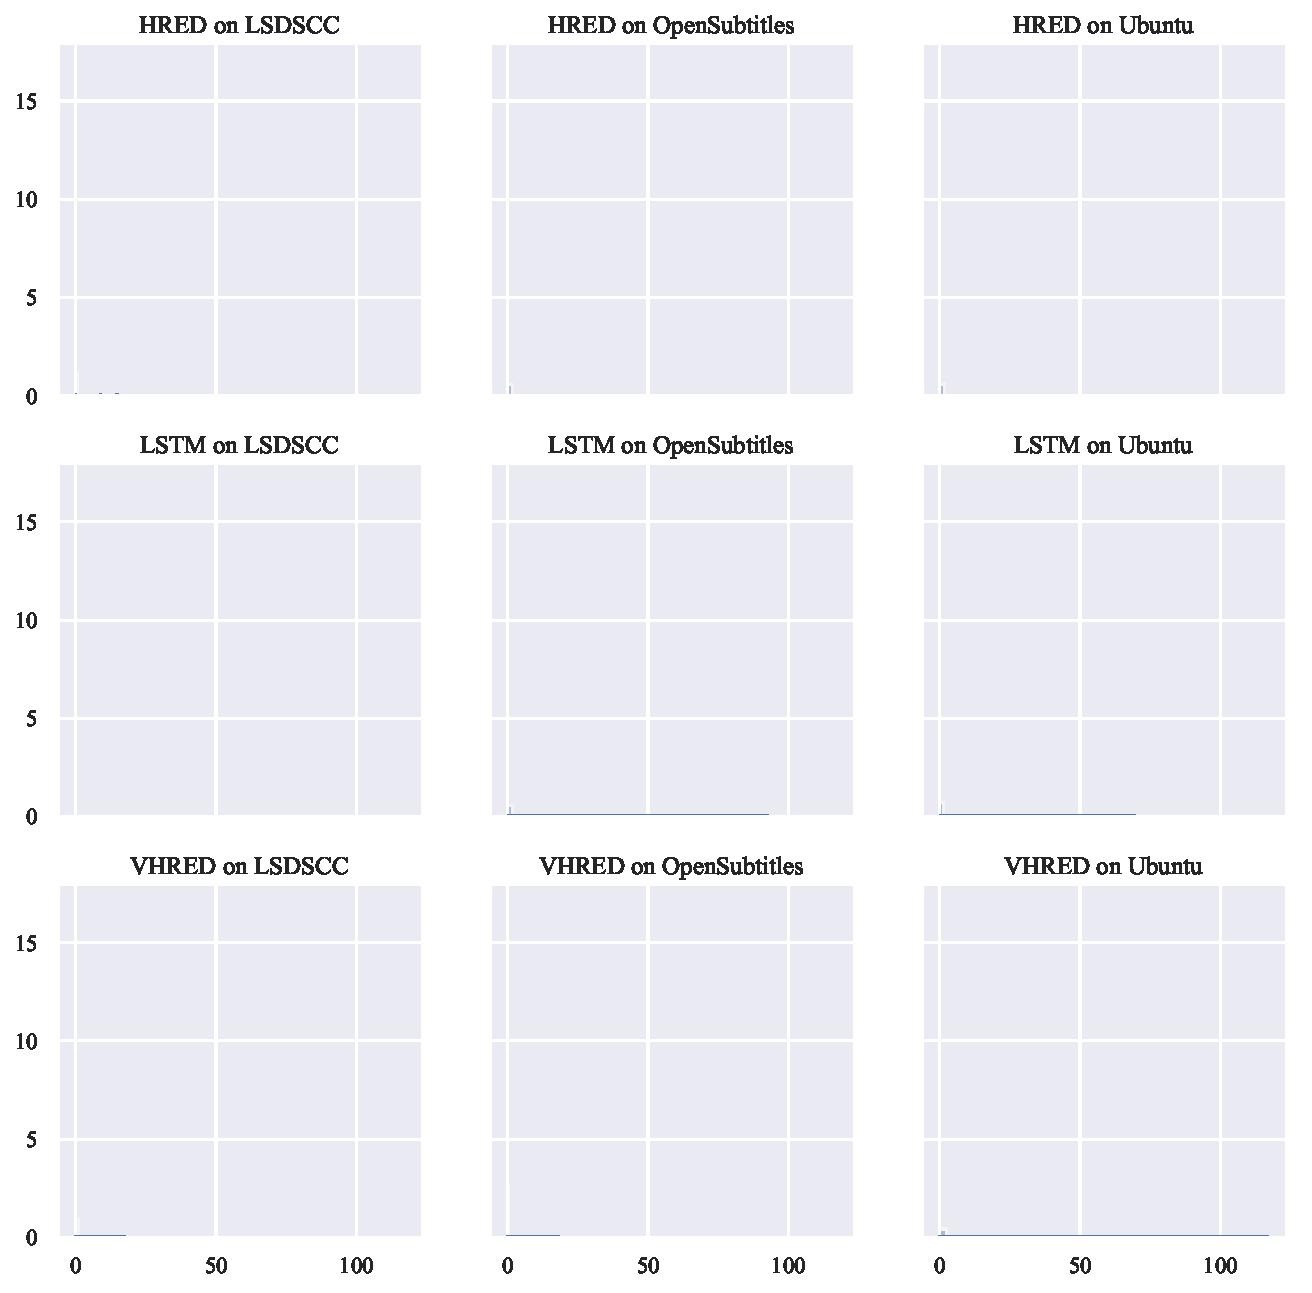
\includegraphics[width=\linewidth]{figure/distplot_grid/rouge_4/plot.pdf}
        \caption{ROUGE-4}
    \end{subfigure}
    \begin{subfigure}{0.33\linewidth}
        \centering
        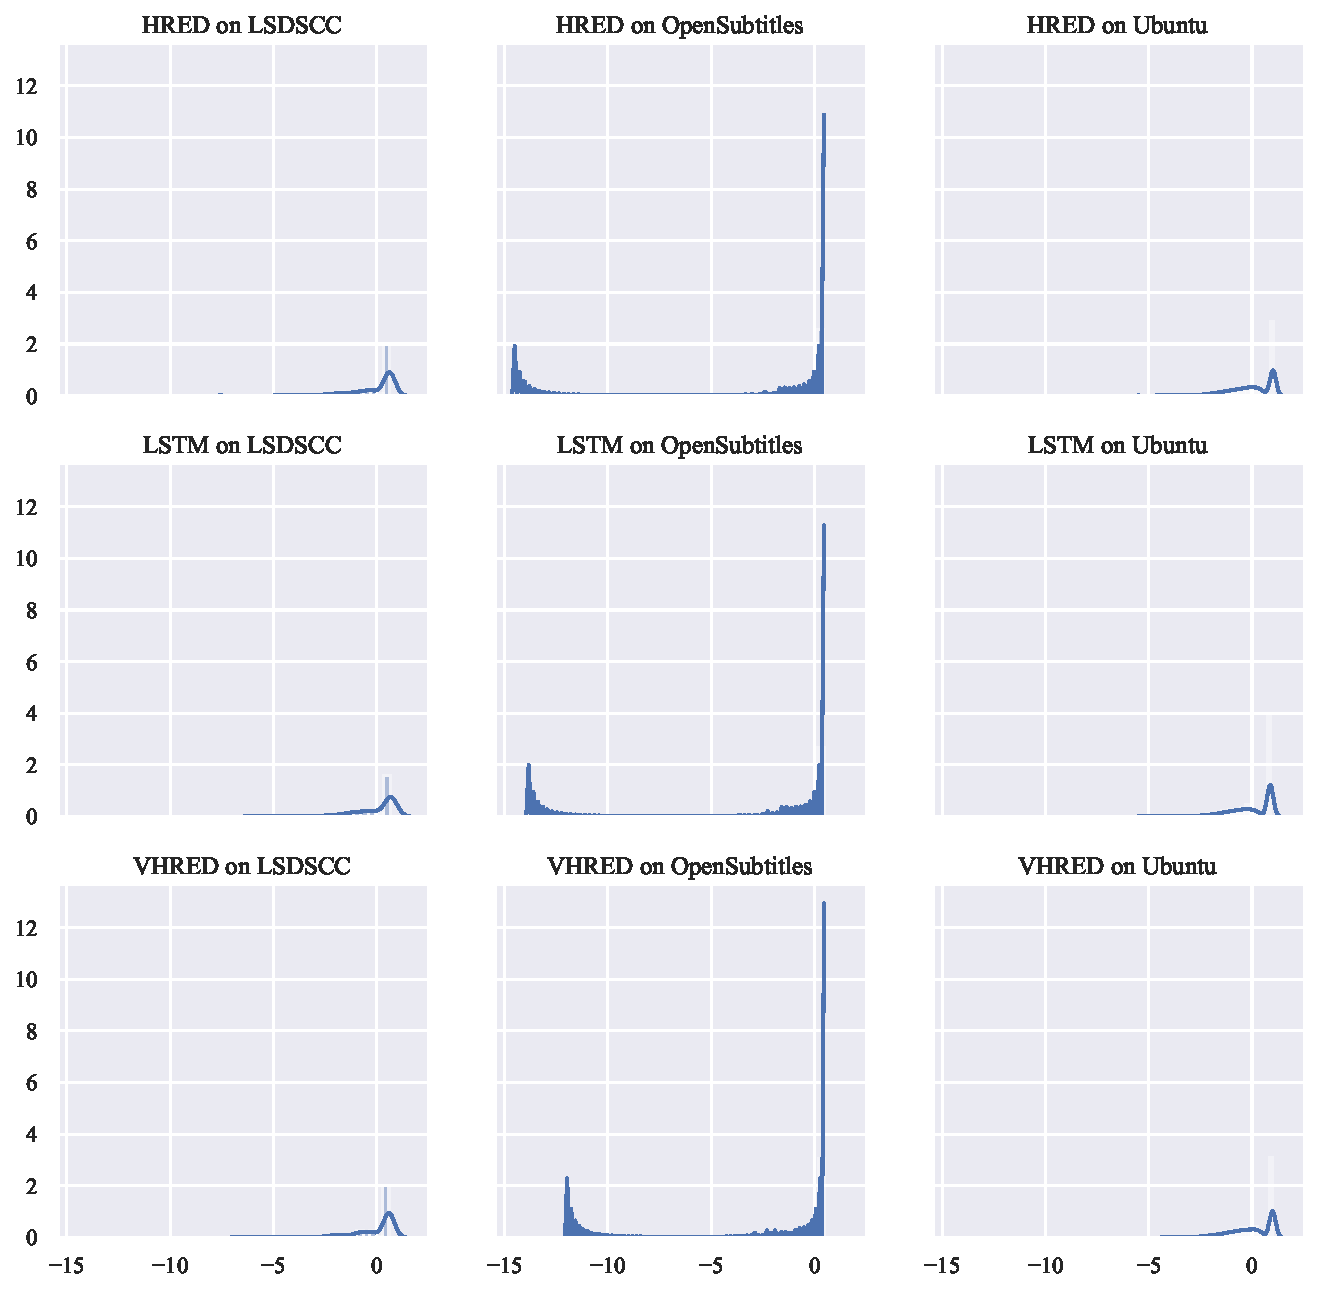
\includegraphics[width=\linewidth]{figure/distplot_grid/distinct_1/plot.pdf}
        \caption{Distinct-1}
    \end{subfigure}%
    \begin{subfigure}{0.33\linewidth}
        \centering
        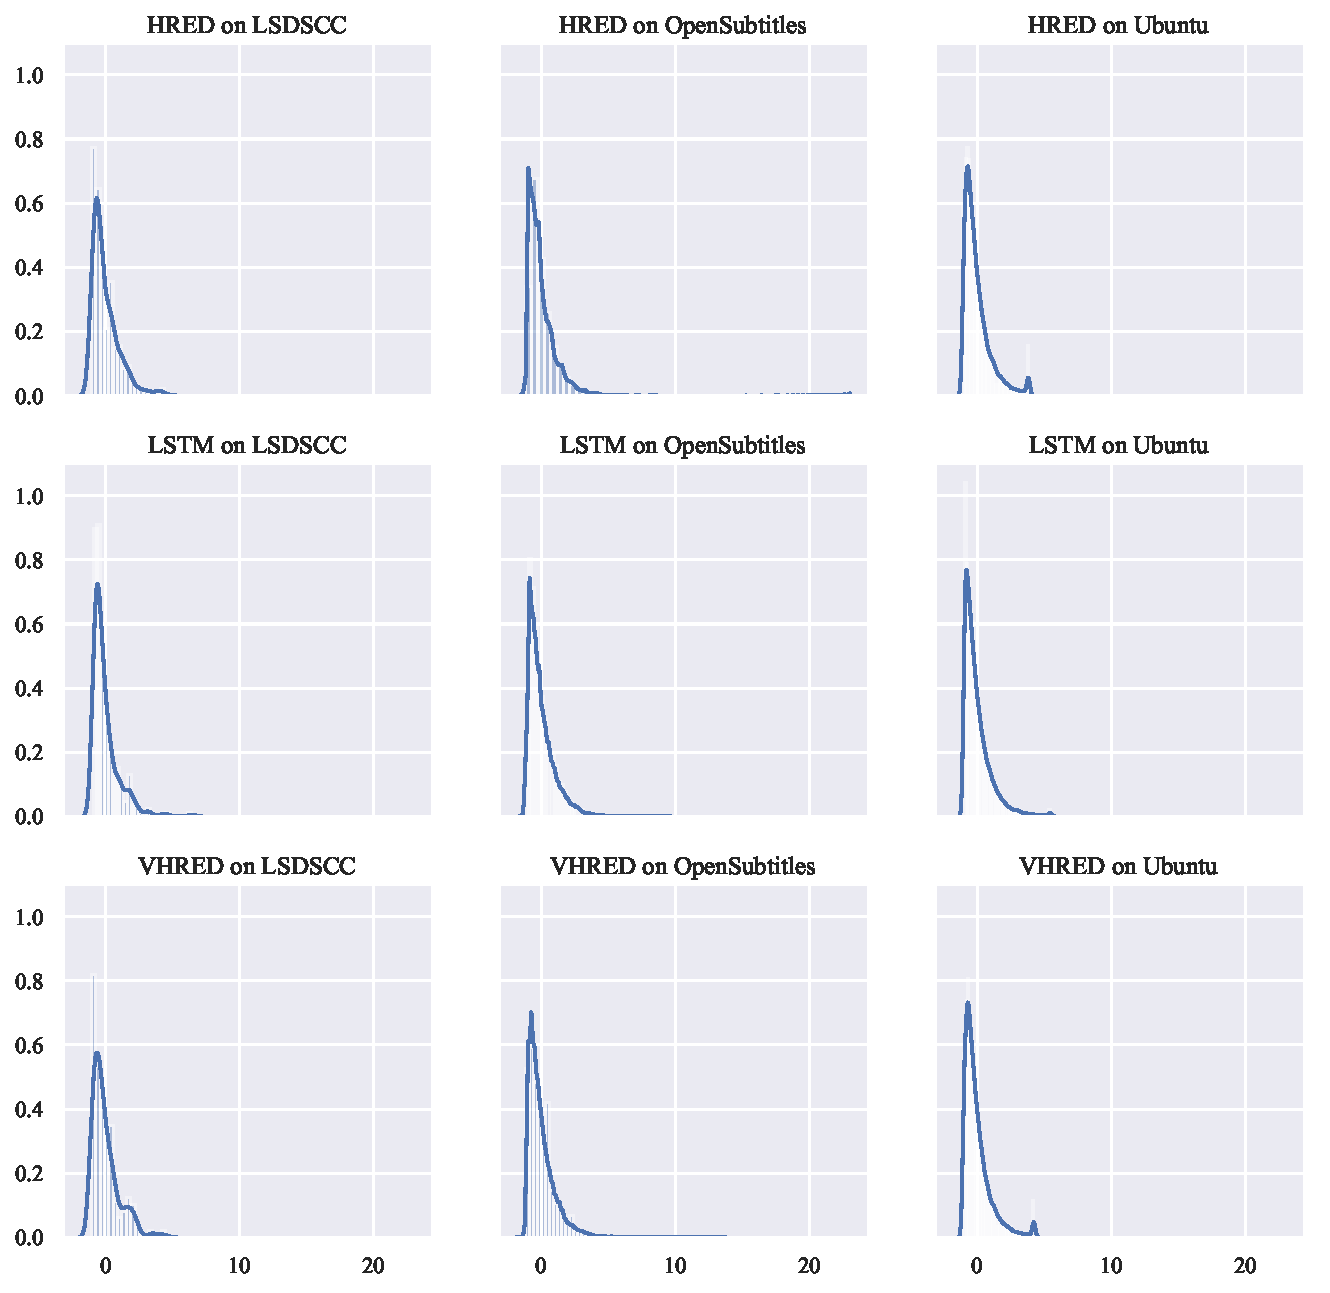
\includegraphics[width=\linewidth]{figure/distplot_grid/utterance_len/plot.pdf}
        \caption{\#words}
    \end{subfigure}%
    \begin{subfigure}{0.33\linewidth}
        \centering
        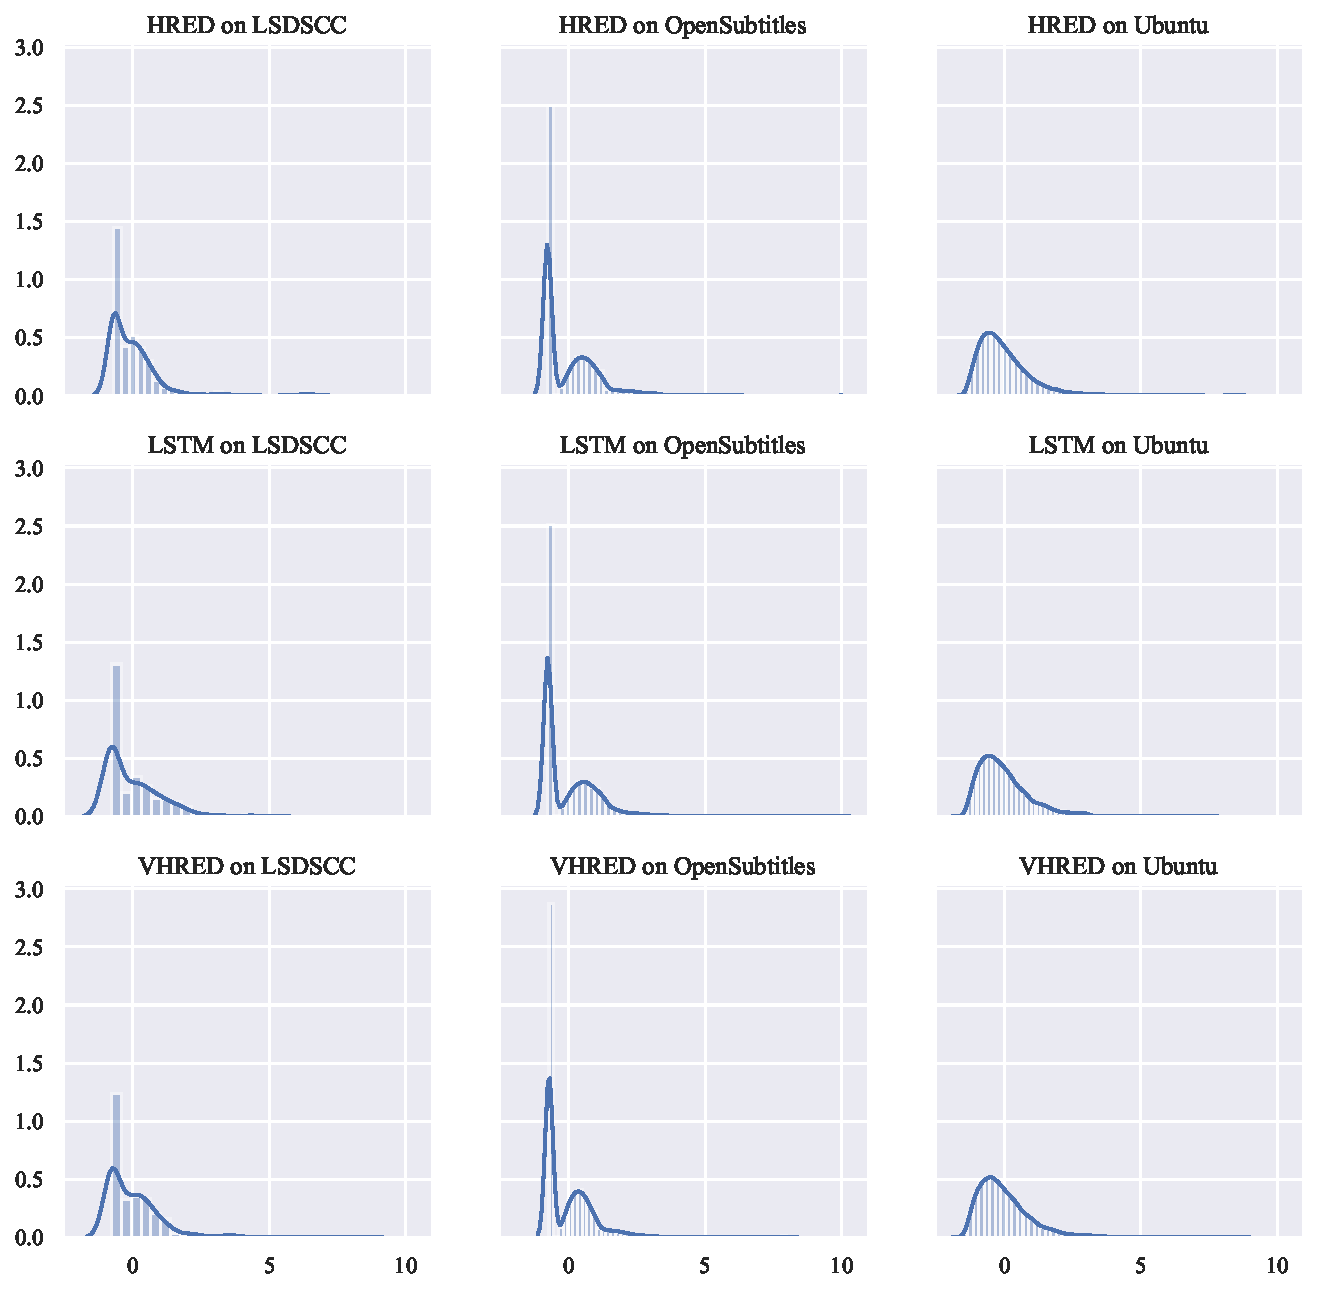
\includegraphics[width=\linewidth]{figure/distplot_grid/rouge_l/plot.pdf}
        \caption{ROUGE-L}
    \end{subfigure}
    \begin{subfigure}{0.33\linewidth}
        \centering
        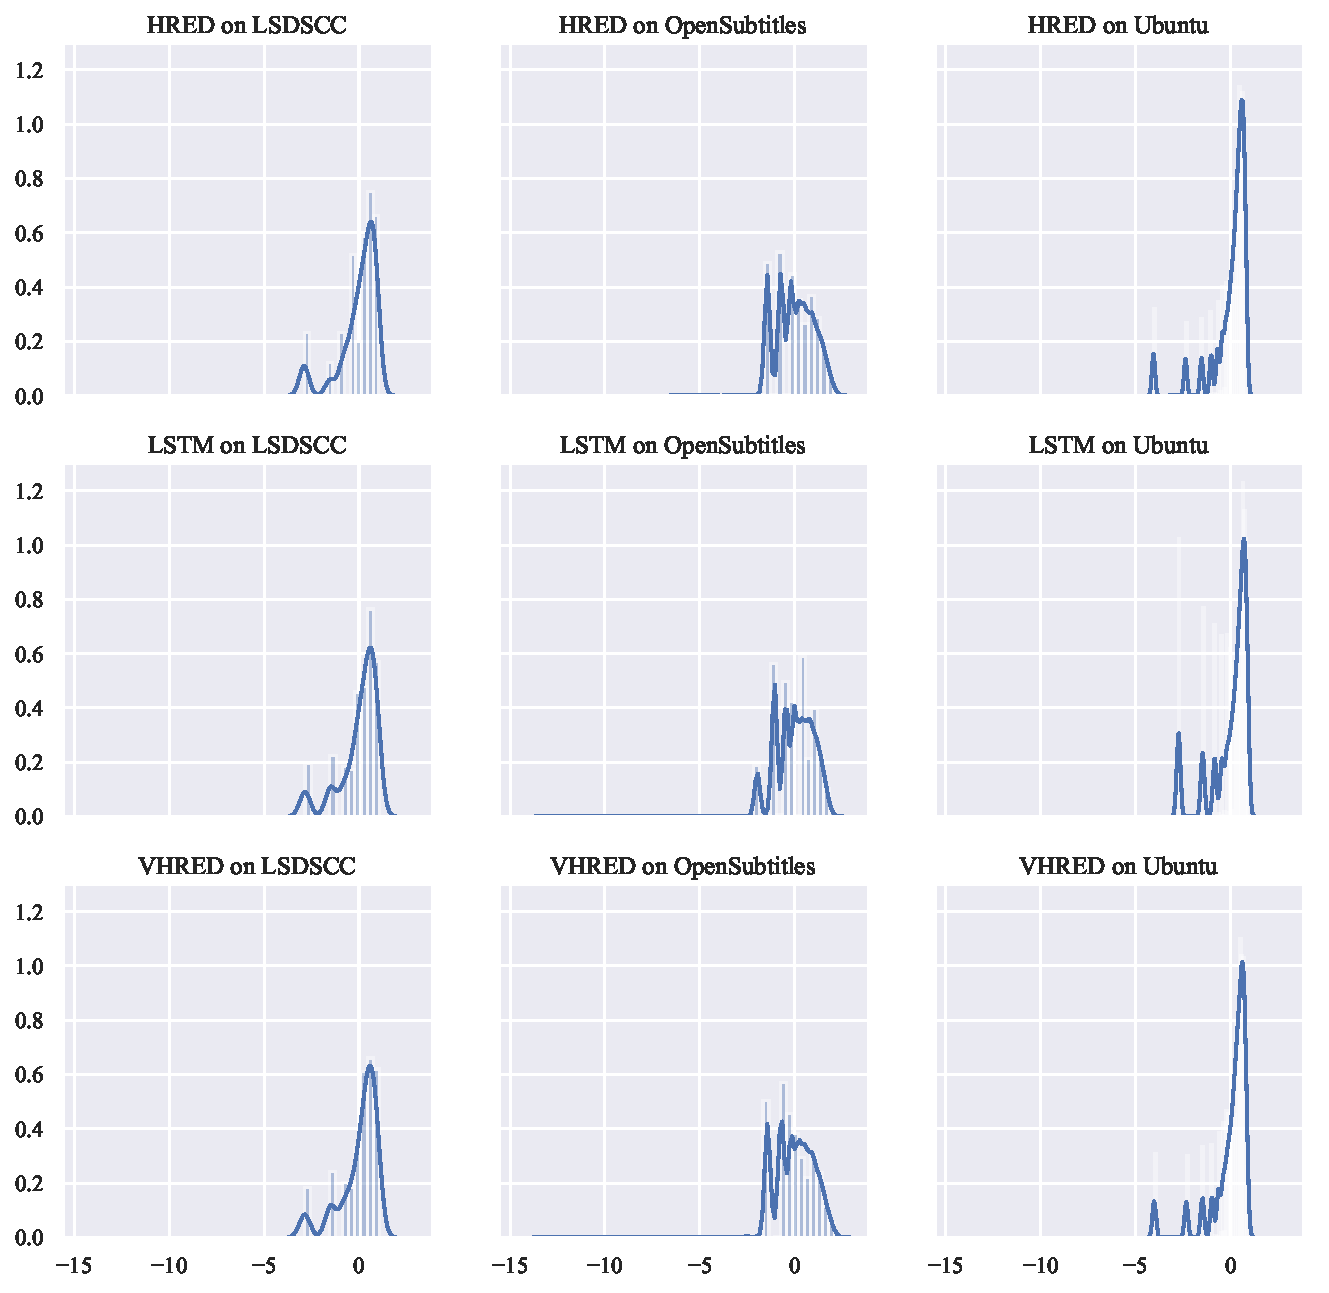
\includegraphics[width=\linewidth]{figure/distplot_grid/distinct_2/plot.pdf}
        \caption{Distinct-2}
    \end{subfigure}%
    \begin{subfigure}{0.33\linewidth}
        \centering
        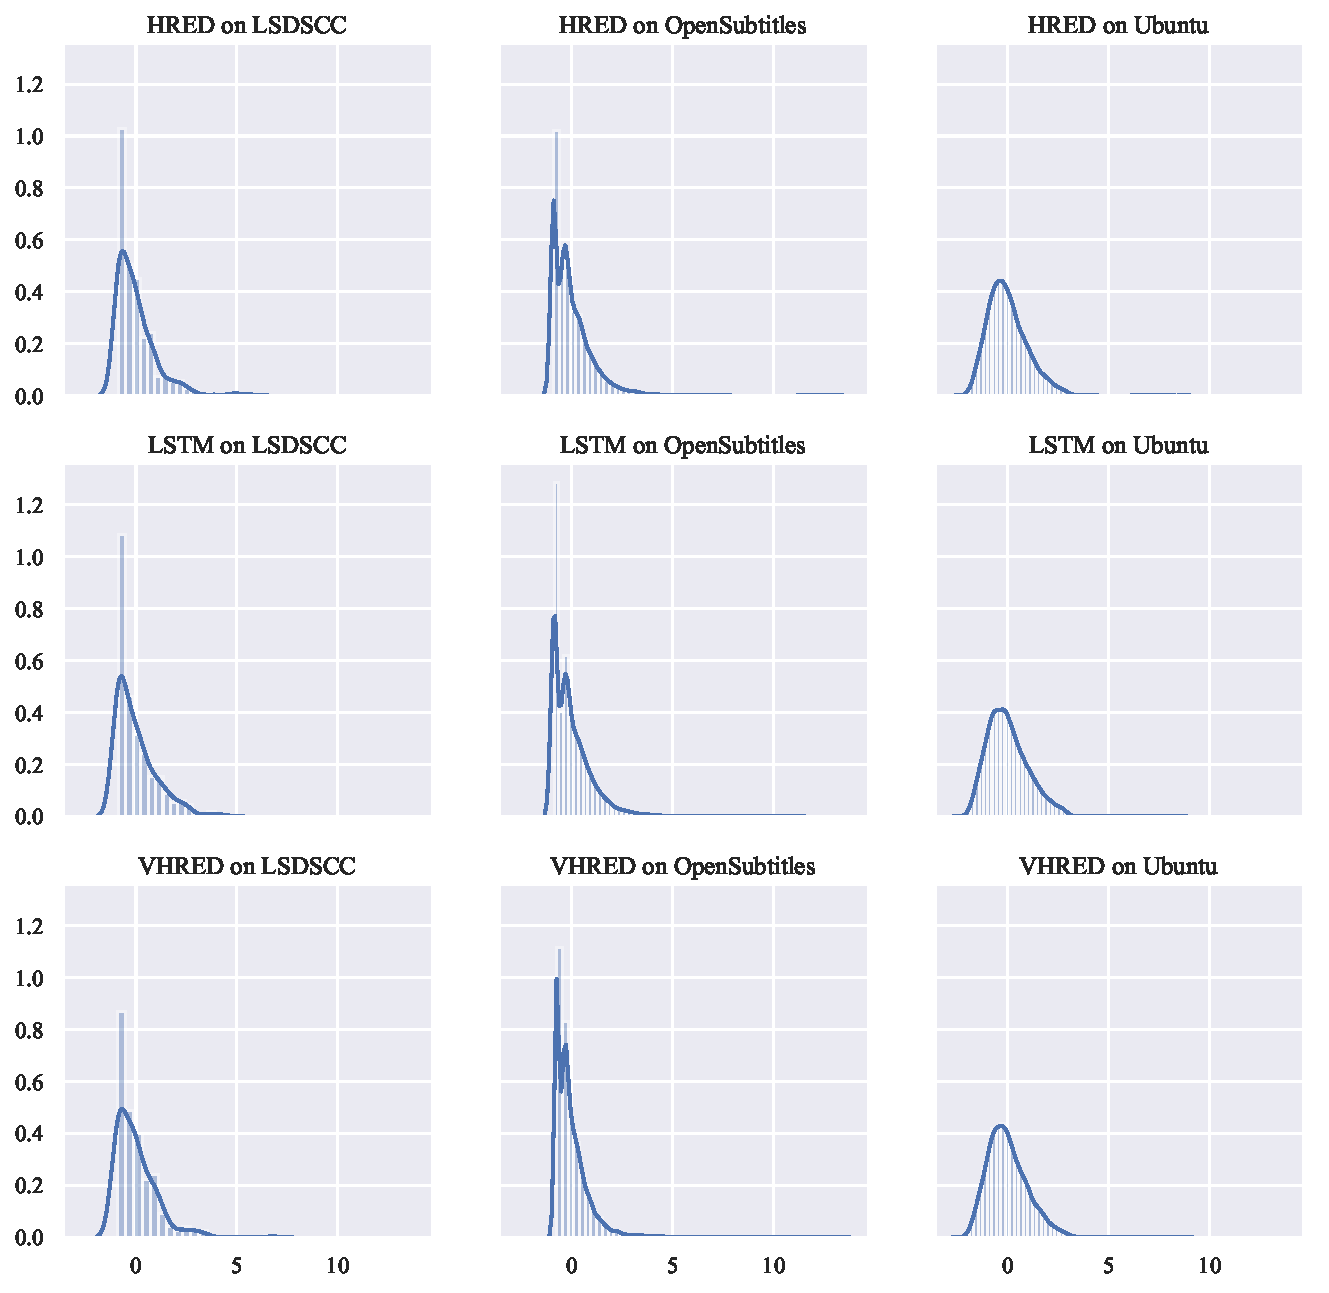
\includegraphics[width=\linewidth]{figure/distplot_grid/meteor/plot.pdf}
        \caption{METEOR}
    \end{subfigure}%
    \begin{subfigure}{0.33\linewidth}
        \centering
        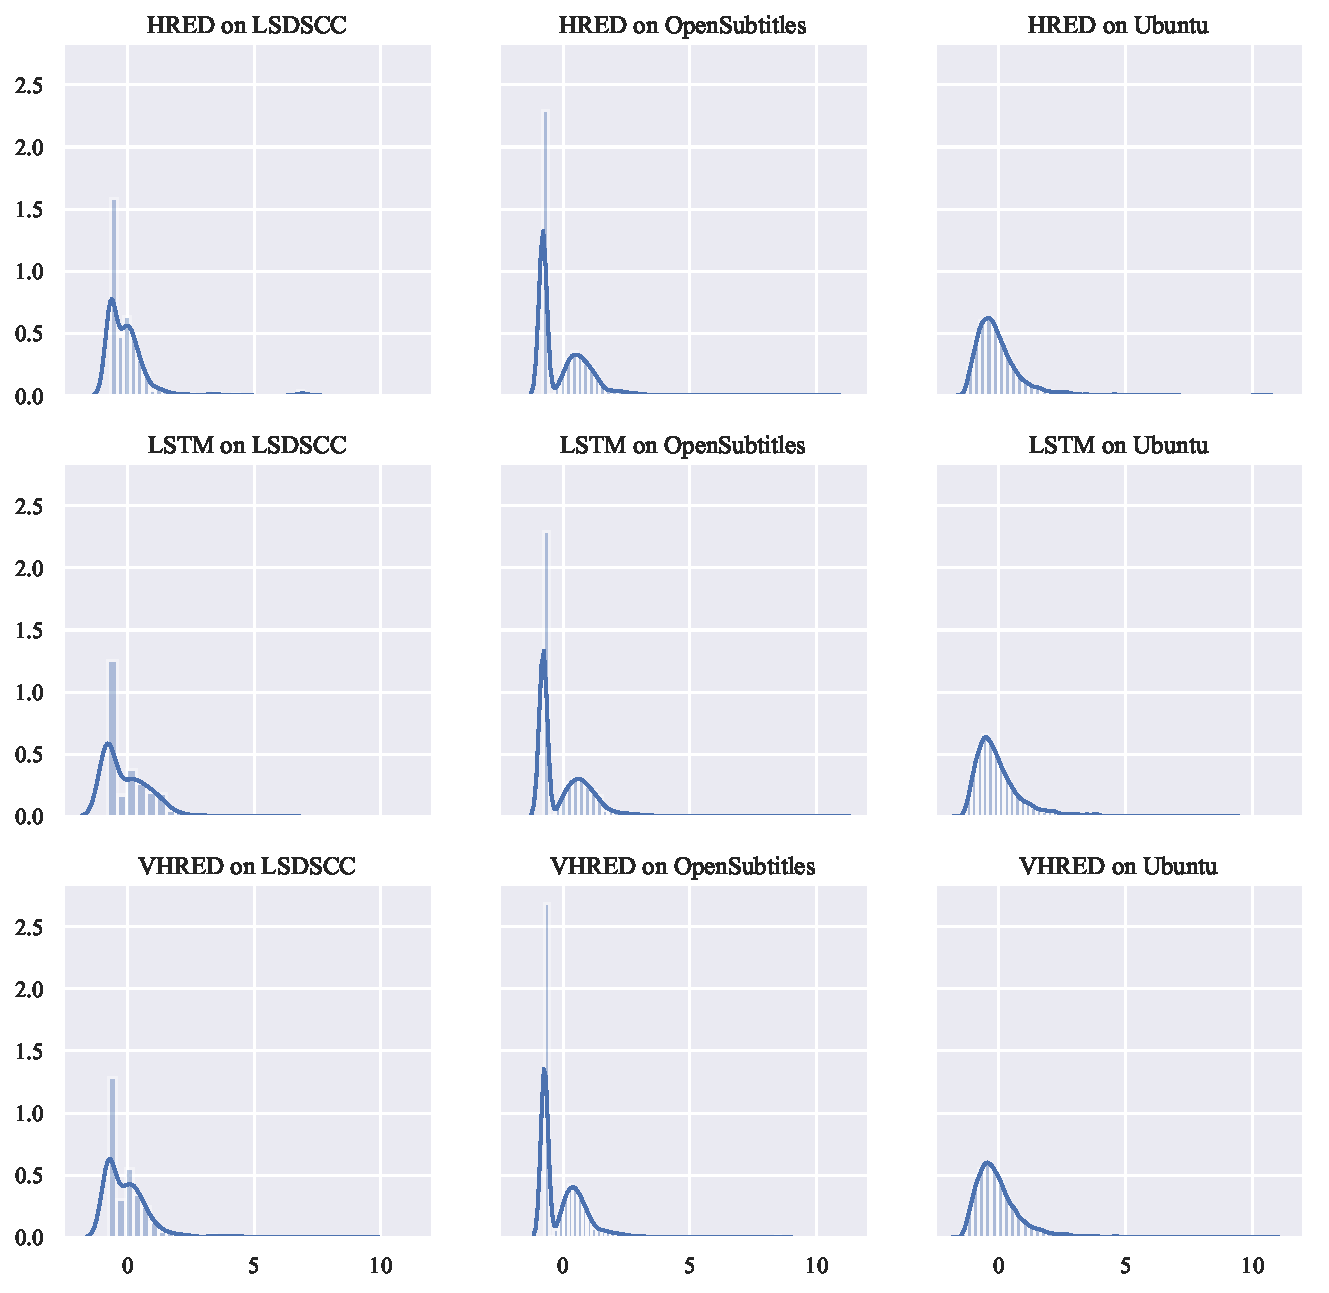
\includegraphics[width=\linewidth]{figure/distplot_grid/rouge_w/plot.pdf}
        \caption{ROUGE-W}
    \end{subfigure}
    \centering
    \caption{句子得分分布二}
\end{figure}

图~\ref{fig:ROUGE_dist}~是ROUGE系列指标的分布图。 从曲线的形状来看,大致可分为两类: ROUGE-1,ROUGE-L,ROUGE-W是一类, ROUGE-2,ROUGE-3,ROUGE-4是一类。 ROUGE-2这类图像的特点是几乎所有句子的得分都集中在均值, 其他区域几乎没有任何句子。 这是因为实验中没有对ROUGE指标做任何平滑处理, 所以除了个别句子外,其他句子都得了零分。 这表明ROUGE-N指标当$N > 1$时捕捉不到任何n-gram重叠。

另一方面,ROUGE-1类指标更像是BLEU-1指标的噪化版本, 它们都是双峰曲线,而且第一个峰值对应的点$(x_1, y_1)$和 第二个峰值对应的点$(x_2, y_2)$都有相似的坐标。 上述现象的原因是所有的响应和参考基本上没有$N > 1$的n-gram重叠, 基于最长公共子序列的匹配退化成了一元词匹配。

% -- Other -- %
% MIT License
% 
% Copyright (c) 2019 Cong Feng
% 
% Permission is hereby granted, free of charge, to any person obtaining a copy
% of this software and associated documentation files (the "Software"), to deal
% in the Software without restriction, including without limitation the rights
% to use, copy, modify, merge, publish, distribute, sublicense, and/or sell
% copies of the Software, and to permit persons to whom the Software is
% furnished to do so, subject to the following conditions:
% 
% The above copyright notice and this permission notice shall be included in all
% copies or substantial portions of the Software.
% 
% THE SOFTWARE IS PROVIDED "AS IS", WITHOUT WARRANTY OF ANY KIND, EXPRESS OR
% IMPLIED, INCLUDING BUT NOT LIMITED TO THE WARRANTIES OF MERCHANTABILITY,
% FITNESS FOR A PARTICULAR PURPOSE AND NONINFRINGEMENT. IN NO EVENT SHALL THE
% AUTHORS OR COPYRIGHT HOLDERS BE LIABLE FOR ANY CLAIM, DAMAGES OR OTHER
% LIABILITY, WHETHER IN AN ACTION OF CONTRACT, TORT OR OTHERWISE, ARISING FROM,
% OUT OF OR IN CONNECTION WITH THE SOFTWARE OR THE USE OR OTHER DEALINGS IN THE
% SOFTWARE.

\begin{figure}[H]
    \begin{subfigure}{0.4\linewidth}
        \centering
        \includegraphics[width=\linewidth]{figure/barplot/distinct_1/plot.pdf}
        \caption{Distinct-1}
        \label{fig:distinct_1_system}
    \end{subfigure}%
    \begin{subfigure}{0.4\linewidth}
        \centering
        \includegraphics[width=\linewidth]{figure/barplot/distinct_2/plot.pdf}
        \caption{Distinct-2}
        \label{fig:distinct_2_system}
    \end{subfigure}
    \begin{subfigure}{0.4\linewidth}
        \centering
        \includegraphics[width=\linewidth]{figure/barplot/utterance_len/plot.pdf}
        \caption{\#words}
        \label{fig:words_system}
    \end{subfigure}%
    \begin{subfigure}{0.4\linewidth}
        \centering
        \includegraphics[width=\linewidth]{figure/barplot/meteor/plot.pdf}
        \caption{METEOR}
        \label{fig:meteor_system}
    \end{subfigure}
    \centering
    \caption{Distinct-N,\#words和METEOR的系统得分}
    \label{fig:Other_system}
\end{figure}

图~\ref{fig:Other_dist}~是Distinct-N,METEOR和\#words的分布图。 Distinct-1的分布呈现两极分化, 在均值附近和均值右边较远处都聚集了大量句子。 Distinct-N的分母是句子的长度(\#words), 分子是句子中互不相同的n-gram数量。 从图~\ref{fig:words_dist}~来看,句子的长度集中在均值附近, 长于均值的句子比短于均值的句子多, 这表明Distinct-N的值主要受分子影响。 Distinct-1的曲线表明,极大部分句子的各异的单词数量都接近平均值, 但也有少部分句子各异的单词数量远远小于平均值。
% -- Distinct-2 -- %
Distinct-2的图像没有出现两极分化, 这是因为二元词的空间比一元词的空间更大, 一个句子互不相同的二元词通常多于互不相同的一元词。 图像的特点是:
\begin{enumerate}
    \item 大部分句子集中在高于均值的一片区域。
    \item 个别低于均值的区间聚集了大量句子。
\end{enumerate}
这可以理解为模型在应对不同的消息时, 生成的句子质量不一,对一部分消息产生了多样的响应, 对另一部分消息却产生了单调的响应。

% -- METEOR -- %
尽管通常被归类成基于词重叠的指标, METEOR的图像表现出了和其他基于词重叠的指标(BLEU,ROUGE)相当不同的性质。 它似乎能区分不同响应的质量,并且和句子长度有着某种联系。 图像在均值的右侧表现出指数衰减, 在左侧则是一个尖锐的单峰。 本质上,METEOR是基于一元词匹配的, 但是本文尚不清楚METEOR的多种匹配模块,对齐算法和惩罚系数如何 使它的分布变得与BLEU-1等指标的分布如此不同。

% -- Conclusion -- %
本节的分析结果是从OpenSubtitles和HRED的组合中得出的, 并不能完全代表所有组合下的指标分布情况。 观察附录~\ref{ch:metric_dist}可发现, 一般来说, 分布的全局形状由指标所使用的特征决定, 分布的局部形状由训练所用的数据集决定, 分布的局部数值,如峰值,由具体的模型决定。

% ---------------- %
% -- Discussion -- %
% ---------------- %
\section{结果与讨论}\label{sec:result_and_discussion}
% -- System Level -- %
系统层面的分析表明,数据集对指标得分的影响普遍大于模型的影响, 表现为同一个数据集上的模型得分比较接近, 同一个模型在不同数据集上的得分相差较远。 不排除某些极端情况,但是一般来说,数据集的影响是决定性的。 此外,有些指标能对同一个数据集上的模型产生差别很大的分数, 另外一些指标则倾向于给不同模型相近的分数。

% -- Utterance Level -- %
句子层面的分析表明不同指标的分布形态各异, 某些指标的分布有着相似的形态,它们和其他指标的分布形成了鲜明对比。 比如基于词嵌入的指标和ADEM指标的分布非常相似, 呈现类似高斯分布的钟型曲线。 和一元词匹配有关的BLEU-1, ROUGE-1,ROUGE-L以及ROUGE-W也有着相似的分布, 图像是不对称的双峰曲线。 本文对分布的相似性的结论是通过观察图像得出的, 更为严谨的做法是计算两个分布的相关系数,如皮尔逊相关系数等等, 本文把基于数据的严谨论证留给后续研究。 指标分布的不一致性在一定程度上解释了模型在系统层面性能的不一致性。

% -- Model -- %
上述经验性的结论反映了几个问题。 从模型的角度来看,基于Seq2Seq框架的模型普遍采用最大化训练样本的对数概率作为目标函数, 所以本质上,模型是数据集的条件概率分布的拟合器。 这意味着如果数据集的噪声很大,那么模型的输出质量会直接受到影响。 使用其他模型框架可能规避此问题, 例如Li等人尝试用对抗生成网络\upcite{Adversarial} 以及强化学习\upcite{deep_RL}生成对话,取得了不错的效果。

% -- Dataset -- %
从数据集的角度来看,实验中的三个数据集都存在大量的错别字, 不规范的语法以及非自然语言符号, 这也许是开放领域对话数据集的共同特点。 如果这些错误样本的比例超过了正确样本的比例, 模型就很难学习到正确的语法或者拼写。 这些数据集大多数来自互联网论坛或者社交媒体, 不同文化背景和生活阅历的人们在这些平台上的对话具有很高的多样性, 这对模型的表达能力提出了挑战。

% -- Metric -- %
从指标的角度来看,基于不同表征的指标有着完全不同的分布, 这导致不同指标在评价同一个模型时出现不一致性。 这种不一致性使评价结果难以解释,甚至阻碍学者们比较各种模型的性能。 本文试图理解模型的响应有没有好坏之分。 在机器翻译领域,系统翻译有好坏之分。本质上, 无论是从语义上还是从表面形式(Surface Form)上,系统翻译越接近参考翻译就越好。 因此机器翻译领域的指标只需要捕捉系统翻译和参考翻译的相似程度即可。 生成式对话则不同,模型的响应没有一概而论的“好坏”之分。 学者们曾经使用BLEU,基于词嵌入的指标\upcite{VHRED}和 困惑度\upcite{GoogleChatbot}去衡量响应的质量, 然而这些度量都不能和人类评价产生很好的相关性。 本文认为,摆在面前的问题或许不是如何提高指标和人类评价的相关性, 而是:“什么样的对话才是好的对话?”

% MIT License
% 
% Copyright (c) 2019 Cong Feng
% 
% Permission is hereby granted, free of charge, to any person obtaining a copy
% of this software and associated documentation files (the "Software"), to deal
% in the Software without restriction, including without limitation the rights
% to use, copy, modify, merge, publish, distribute, sublicense, and/or sell
% copies of the Software, and to permit persons to whom the Software is
% furnished to do so, subject to the following conditions:
% 
% The above copyright notice and this permission notice shall be included in all
% copies or substantial portions of the Software.
% 
% THE SOFTWARE IS PROVIDED "AS IS", WITHOUT WARRANTY OF ANY KIND, EXPRESS OR
% IMPLIED, INCLUDING BUT NOT LIMITED TO THE WARRANTIES OF MERCHANTABILITY,
% FITNESS FOR A PARTICULAR PURPOSE AND NONINFRINGEMENT. IN NO EVENT SHALL THE
% AUTHORS OR COPYRIGHT HOLDERS BE LIABLE FOR ANY CLAIM, DAMAGES OR OTHER
% LIABILITY, WHETHER IN AN ACTION OF CONTRACT, TORT OR OTHERWISE, ARISING FROM,
% OUT OF OR IN CONNECTION WITH THE SOFTWARE OR THE USE OR OTHER DEALINGS IN THE
% SOFTWARE.

\chapter*{结论}\label{ch:conclusion}
\addcontentsline{toc}{chapter}{结论}

% -------------------------- %
% -------- Summary --------- %
% -------------------------- %
\section*{总结}\label{sec:conclusion}
% -- Related Work -- %
本文对生成式对话领域的模型,数据集和指标进行了一次深入考察。
本文首先介绍了本领域的研究现状,
接着介绍了生成式模型的定义,RNN语言模型和Seq2Seq框架。
本文着重介绍了本领域的常见指标,包括基于词重叠的指标,基于词嵌入的指标,
衡量概率语言模型性能的困惑度,以及专门为生成式对话设计的ADEM和RUBER等等。
最后,本文介绍了本领域常用的开放领域对话数据集。

% -- Methodology -- %
在众多模型,数据集和指标中,本文选择了Serban等人在文献\cite{VHRED}
中使用的三个模型HRED,LSTM和VHRED。
在数据集方面,本文选择了公开的,代表了不同领域的三个数据集,
分别是Ubuntu对话数据集,OpenSubtitles和LSDSCC数据集。
在指标方面,本文尽可能涵盖了对话领域使用过或者提出的指标。
本文的主要工作是:
\begin{enumerate}
    \item 在多个数据集上训练多个模型。
    \item 在训练结果上运行多个评价指标。
    \item 对指标进行多种数据分析。
\end{enumerate}
实验配置与文献\cite{HowNot}大致对齐。
实验数据包括多个模型和数据集的组合在不同指标上的得分,以及这些模型输出的响应。
由于时间关系,本文只分析了得分的数据,把分析模型的输出留给后续工作。

% -- Experiment -- %
本文分析了系统层面得分和句子层面得分。
系统层面得分是是对模型在一个数据集上的表现的粗粒度考察,
它可能掩盖了一些事实,
但是便于综合考察模型、数据集和指标三者的整体关系。
参照文献\cite{HowNot},本文对指标进行分组,并围绕各组指标进行分析。
各模型的系统层面得分随着数据集的变化和指标的变化有较大差异,
比较稳定的是同一个数据集上各模型的排名,
一般HRED和VHRED比LSTM得分高。
模型在Ubuntu对话数据集上的各项指标通常更好。
除了实验过程本身的噪音外,
主要的原因是开放领域对话数据集的特征变化大,
模型无法将一个数据集上的性能完全迁移到另一个数据集上。

本文还考察了句子层面得分的单变量分布,
从分布图像中发现了指标的集群现象。
集群现象反映了提取相同特征的指标有着相似的分布。
指标分布的图像大致可分为两类:
\begin{enumerate}
    \item 基于词嵌入的指标的图像是钟型曲线,接近高斯分布。
    \item 基于词重叠的指标的图像是不对称的双峰曲线,大量句子集中在均值附近很小的范围。
\end{enumerate}
本文尚不清楚指标的具体算法或者模型是如何影响分布的,有待后续研究。

% -------------------------- %
% ------ Future Work ------- %
% -------------------------- %
\section*{展望}\label{sec:future_work}
在实验结论的基础上,
本文对生成式对话领域的模型,数据集以及指标提出几点展望。

% -- Model -- %
在模型方面,尽管Seq2Seq框架在机器翻译领域取得成功,
但是在更加困难的对话响应生成领域,它的表达力遇到了瓶颈。
因此,本文建议尝试新的模型体系结构。
Transformer框架\upcite{Transformer}是一种在大规模语料库上预训练的,
能根据特定任务微调的语言模型。
基于Transformer框架的模型在多项自然语言处理任务中取得了目前最高水平,
将其应用到生成式对话领域有望提升模型的性能。
其他值得尝试的体系结构有对抗生成网络和强化学习,
Li等人在这方面获得了意义重大的进展\upcite{deep_RL,Adversarial}。
另一方面,本文建议在模型中添加额外的特征,比如感情色彩\upcite{ECM},
主题词\upcite{Topic_Aware}和对话者身份信息\upcite{persona}等等。
添加额外特征能使模型的输出在这些特征上具有一致性,从而提高人类评价的得分。

% -- Dataset -- %
在数据集方面,通过在线聊天收集的对话样本具有很高的多样性,
这和人类在这种开放和匿名的平台的表现有密切联系。
从概率的角度,数据集的样本分布可以看作是非常多个随机变量的叠加,
如果这些随机变量都是独立同分布的话,
整个数据集的样本分布就趋向于高斯分布。
面对复杂的数据集,本文建议使用概率统计工具分析它在
多个方面的分布情况,例如情感分布,对话轮数分布等等。
了解数据集的统计特征有助于理解在这个数据集上训练模型的难度。

% -- Metric -- %
在指标方面,本文的实验结论补充了文献\cite{HowNot}的结论。
为了深入理解对话生成问题,本文提出一个问题:什么样的对话才是好的对话?
这是一个重要的问题,它不仅指导着指标的构建,还决定了模型优化的方向。
人类的对话是在自然环境和社会环境中进化出的一种语言现象,
它根据不同场合和参与者的变化而变化的,非常复杂。
所以这个问题可能难以回答,甚至没有普适性的答案,

从实用的角度,
可以通过实验发现在某些数据集上好的对话应有的特征。
直观的来说,
在Ubuntu对话数据集上,对话以“提问-解决问题”为主,
好的对话应该能帮助人们解决问题,
因此应该和具体的技术话题有较高的相关性;
在Twitter对话数据集上,
对话主要是人们发布的个人状态信息,经常带有感情色彩,
而且人们期望从响应中看到相同的话题或者新奇的事物,
因此好的对话应该考虑情感因素,
关注主题的同时又具有一定的多样性,
在LSDSCC数据集上,对话主要是人们发表对电影的点评,
人们一般希望和看过同类电影的人一起讨论,
虽然有时候有人会发表极端的评价,
但是从长远来看,人们不希望总是看到极端的评价,
所以好的对话应该是对相关电影的中肯评价,
并且带有个性化看法。

综上所述,不妨给“什么样的对话才是好的对话”加上“在某个数据集上”的限定词,
从某个数据集中发现好的对话的模式,
然后设计出能捕获这些模式的指标,
并用它评价在该数据集上训练的模型。
具体来说,本文提出把“设计出和人类评价相关度高的指标”这一任务分解为若干个小任务:
\begin{enumerate}
    \item 把问题限制在某个数据集上。
    \item 找出这个数据集上人类评价高的对话所具有的特征。
    \item 设计出能准确捕获这些特征的指标。
    \item 用人类评价验证指标在对应数据集上的有效性。
\end{enumerate}

本文把这个方法称为数据驱动的指标构建法(Data-Driven Metric Construction)。
必须指出,第二步和第三步具有很大的难度。
第二步一般需要人类评价员对数据集的样本打分,
这将导致带有人类评价的样本比较稀少,
要求指标的泛化能力比较强\upcite{ADEM}。
第三步涉及的特征比较抽象,要求指标的建模能力比较强。


% 致谢
% MIT License
% 
% Copyright (c) 2022 cgsdfc
% 
% Permission is hereby granted, free of charge, to any person obtaining a copy
% of this software and associated documentation files (the "Software"), to deal
% in the Software without restriction, including without limitation the rights
% to use, copy, modify, merge, publish, distribute, sublicense, and/or sell
% copies of the Software, and to permit persons to whom the Software is
% furnished to do so, subject to the following conditions:
% 
% The above copyright notice and this permission notice shall be included in all
% copies or substantial portions of the Software.
% 
% THE SOFTWARE IS PROVIDED "AS IS", WITHOUT WARRANTY OF ANY KIND, EXPRESS OR
% IMPLIED, INCLUDING BUT NOT LIMITED TO THE WARRANTIES OF MERCHANTABILITY,
% FITNESS FOR A PARTICULAR PURPOSE AND NONINFRINGEMENT. IN NO EVENT SHALL THE
% AUTHORS OR COPYRIGHT HOLDERS BE LIABLE FOR ANY CLAIM, DAMAGES OR OTHER
% LIABILITY, WHETHER IN AN ACTION OF CONTRACT, TORT OR OTHERWISE, ARISING FROM,
% OUT OF OR IN CONNECTION WITH THE SOFTWARE OR THE USE OR OTHER DEALINGS IN THE
% SOFTWARE.

\chapter*{致谢}
\addcontentsline{toc}{chapter}{致谢}
我要感谢我的毕业设计指导老师荣文戈副教授。
在毕设一开始,我因为考研、重修课程等事情无法立刻投入工作,荣老师对此表示了极大的理解,对此我深表感谢。
在中期报告前的一个月,荣老师给了我关键的支持:他不但给了我两台学院的服务器,
而且还在紧缺的实验室工位中给我安排了一个。
在此后的毕设工作中,他不断根据我的工作汇报为我的毕设提供切实有效的指导。
没有荣老师的帮助和指导,我的毕设工作可能完全走不上正轨。
荣老师的谆谆教导和谦谦君子之风让我感受到老一辈北航人一脉相承的渊博与儒雅,能在他的指导下完成毕设是我的荣幸。

我要感谢我们计算机学院对毕设工作的高度重视和大力支持。
学院早在去年10月就召开了毕设动员大会,不久之后就组织了全学院的开题报告。
据我所知,全校范围内恐怕没有比我们学院更早的了。得益于此,我们比别的学院多出几乎半年时间做准备。
我非常感谢高小鹏院长等学院领导对我们毕设的重视,
高院长在毕设动员大会上指出了毕设过程中可能会遇到的种种挫折,告诫我们要对自己负责,要多和导师沟通等等,
这些都是我在毕设过程中一直受用的。
开题报告、中期报告和毕设答辩等环节有赖于学院的全体教职工的辛勤付出,
感谢他们不惜牺牲宝贵的休息时间来为我们这些初出茅庐的本科生提出意见。

我还想感谢密码学课程的郭华老师,她在我毕业这年教会我信息安全的重要性。
感谢G951的各位学长学姐,感谢他们在“五一”劳动节和我一起看电影,这是一段美好的回忆。
感谢学生三公寓的楼管阿姨,她总是把我们当成自己的孩子看待,热心帮助我们,关心我们。
感谢校车司机,他们一天出车十几趟,将满载的师生安全送达,还将我遗失在校车上的背包完璧归赵。
感谢在某个暴雨的凌晨,一位不知名的博士学长撑着伞送我回宿舍……即使是陌生人也带来了温暖。

最后,我要感谢我的父母:他们无私和博大的关爱,我永远铭记于心。

% 参考文献
% MIT License
% 
% Copyright (c) 2022 cgsdfc
% 
% Permission is hereby granted, free of charge, to any person obtaining a copy
% of this software and associated documentation files (the "Software"), to deal
% in the Software without restriction, including without limitation the rights
% to use, copy, modify, merge, publish, distribute, sublicense, and/or sell
% copies of the Software, and to permit persons to whom the Software is
% furnished to do so, subject to the following conditions:
% 
% The above copyright notice and this permission notice shall be included in all
% copies or substantial portions of the Software.
% 
% THE SOFTWARE IS PROVIDED "AS IS", WITHOUT WARRANTY OF ANY KIND, EXPRESS OR
% IMPLIED, INCLUDING BUT NOT LIMITED TO THE WARRANTIES OF MERCHANTABILITY,
% FITNESS FOR A PARTICULAR PURPOSE AND NONINFRINGEMENT. IN NO EVENT SHALL THE
% AUTHORS OR COPYRIGHT HOLDERS BE LIABLE FOR ANY CLAIM, DAMAGES OR OTHER
% LIABILITY, WHETHER IN AN ACTION OF CONTRACT, TORT OR OTHERWISE, ARISING FROM,
% OUT OF OR IN CONNECTION WITH THE SOFTWARE OR THE USE OR OTHER DEALINGS IN THE
% SOFTWARE.

\cleardoublepage
\phantomsection
\addcontentsline{toc}{chapter}{参考文献}
\bibliography{content/all}
\cleardoublepage


% 附录
\appendix
% MIT License
% 
% Copyright (c) 2022 cgsdfc
% 
% Permission is hereby granted, free of charge, to any person obtaining a copy
% of this software and associated documentation files (the "Software"), to deal
% in the Software without restriction, including without limitation the rights
% to use, copy, modify, merge, publish, distribute, sublicense, and/or sell
% copies of the Software, and to permit persons to whom the Software is
% furnished to do so, subject to the following conditions:
% 
% The above copyright notice and this permission notice shall be included in all
% copies or substantial portions of the Software.
% 
% THE SOFTWARE IS PROVIDED "AS IS", WITHOUT WARRANTY OF ANY KIND, EXPRESS OR
% IMPLIED, INCLUDING BUT NOT LIMITED TO THE WARRANTIES OF MERCHANTABILITY,
% FITNESS FOR A PARTICULAR PURPOSE AND NONINFRINGEMENT. IN NO EVENT SHALL THE
% AUTHORS OR COPYRIGHT HOLDERS BE LIABLE FOR ANY CLAIM, DAMAGES OR OTHER
% LIABILITY, WHETHER IN AN ACTION OF CONTRACT, TORT OR OTHERWISE, ARISING FROM,
% OUT OF OR IN CONNECTION WITH THE SOFTWARE OR THE USE OR OTHER DEALINGS IN THE
% SOFTWARE.

\chapter{系统得分在数据集和模型上的分布}\label{ch:dataset_system_dist}
\begin{figure}[H]
    \begin{subfigure}{0.4\linewidth}
        \centering
        \includegraphics[width=\linewidth]{figure/barplot/bleu_1/plot.pdf}
        \caption{BLEU-1}
    \end{subfigure}%
    \begin{subfigure}{0.4\linewidth}
        \centering
        \includegraphics[width=\linewidth]{figure/barplot/bleu_2/plot.pdf}
        \caption{BLEU-2}
    \end{subfigure}
    \begin{subfigure}{0.4\linewidth}
        \centering
        \includegraphics[width=\linewidth]{figure/barplot/bleu_3/plot.pdf}
        \caption{BLEU-3}
    \end{subfigure}%
    \begin{subfigure}{0.4\linewidth}
        \centering
        \includegraphics[width=\linewidth]{figure/barplot/bleu_4/plot.pdf}
        \caption{BLEU-4}
    \end{subfigure}
    \centering
    \caption{BLEU的系统得分}
    \label{fig:BLEU_system}
\end{figure}

% MIT License
% 
% Copyright (c) 2022 cgsdfc
% 
% Permission is hereby granted, free of charge, to any person obtaining a copy
% of this software and associated documentation files (the "Software"), to deal
% in the Software without restriction, including without limitation the rights
% to use, copy, modify, merge, publish, distribute, sublicense, and/or sell
% copies of the Software, and to permit persons to whom the Software is
% furnished to do so, subject to the following conditions:
% 
% The above copyright notice and this permission notice shall be included in all
% copies or substantial portions of the Software.
% 
% THE SOFTWARE IS PROVIDED "AS IS", WITHOUT WARRANTY OF ANY KIND, EXPRESS OR
% IMPLIED, INCLUDING BUT NOT LIMITED TO THE WARRANTIES OF MERCHANTABILITY,
% FITNESS FOR A PARTICULAR PURPOSE AND NONINFRINGEMENT. IN NO EVENT SHALL THE
% AUTHORS OR COPYRIGHT HOLDERS BE LIABLE FOR ANY CLAIM, DAMAGES OR OTHER
% LIABILITY, WHETHER IN AN ACTION OF CONTRACT, TORT OR OTHERWISE, ARISING FROM,
% OUT OF OR IN CONNECTION WITH THE SOFTWARE OR THE USE OR OTHER DEALINGS IN THE
% SOFTWARE.

\begin{figure}[H]
    \begin{subfigure}{0.33\linewidth}
        \centering
        \includegraphics[width=\linewidth]{figure/distplot_grid/bleu_4/plot.pdf}
        \caption{BLEU-4}
    \end{subfigure}%
    \begin{subfigure}{0.33\linewidth}
        \includegraphics[width=\linewidth]{figure/distplot_grid/adem/plot.pdf}
        \centering
        \caption{ADEM}
    \end{subfigure}%
    \begin{subfigure}{0.33\linewidth}
        \centering
        \includegraphics[width=\linewidth]{figure/distplot_grid/rouge_4/plot.pdf}
        \caption{ROUGE-4}
    \end{subfigure}
    \begin{subfigure}{0.33\linewidth}
        \centering
        \includegraphics[width=\linewidth]{figure/distplot_grid/distinct_1/plot.pdf}
        \caption{Distinct-1}
    \end{subfigure}%
    \begin{subfigure}{0.33\linewidth}
        \centering
        \includegraphics[width=\linewidth]{figure/distplot_grid/utterance_len/plot.pdf}
        \caption{\#words}
    \end{subfigure}%
    \begin{subfigure}{0.33\linewidth}
        \centering
        \includegraphics[width=\linewidth]{figure/distplot_grid/rouge_l/plot.pdf}
        \caption{ROUGE-L}
    \end{subfigure}
    \begin{subfigure}{0.33\linewidth}
        \centering
        \includegraphics[width=\linewidth]{figure/distplot_grid/distinct_2/plot.pdf}
        \caption{Distinct-2}
    \end{subfigure}%
    \begin{subfigure}{0.33\linewidth}
        \centering
        \includegraphics[width=\linewidth]{figure/distplot_grid/meteor/plot.pdf}
        \caption{METEOR}
    \end{subfigure}%
    \begin{subfigure}{0.33\linewidth}
        \centering
        \includegraphics[width=\linewidth]{figure/distplot_grid/rouge_w/plot.pdf}
        \caption{ROUGE-W}
    \end{subfigure}
    \centering
    \caption{句子得分分布二}
\end{figure}


% MIT License
% 
% Copyright (c) 2022 cgsdfc
% 
% Permission is hereby granted, free of charge, to any person obtaining a copy
% of this software and associated documentation files (the "Software"), to deal
% in the Software without restriction, including without limitation the rights
% to use, copy, modify, merge, publish, distribute, sublicense, and/or sell
% copies of the Software, and to permit persons to whom the Software is
% furnished to do so, subject to the following conditions:
% 
% The above copyright notice and this permission notice shall be included in all
% copies or substantial portions of the Software.
% 
% THE SOFTWARE IS PROVIDED "AS IS", WITHOUT WARRANTY OF ANY KIND, EXPRESS OR
% IMPLIED, INCLUDING BUT NOT LIMITED TO THE WARRANTIES OF MERCHANTABILITY,
% FITNESS FOR A PARTICULAR PURPOSE AND NONINFRINGEMENT. IN NO EVENT SHALL THE
% AUTHORS OR COPYRIGHT HOLDERS BE LIABLE FOR ANY CLAIM, DAMAGES OR OTHER
% LIABILITY, WHETHER IN AN ACTION OF CONTRACT, TORT OR OTHERWISE, ARISING FROM,
% OUT OF OR IN CONNECTION WITH THE SOFTWARE OR THE USE OR OTHER DEALINGS IN THE
% SOFTWARE.

\chapter{指标的句子层面得分的分布}
\label{ch:metric_dist}
\begin{figure}[H]
    \begin{subfigure}{0.4\linewidth}
        \centering
        \includegraphics[width=\linewidth]{figure/barplot/bleu_1/plot.pdf}
        \caption{BLEU-1}
    \end{subfigure}%
    \begin{subfigure}{0.4\linewidth}
        \centering
        \includegraphics[width=\linewidth]{figure/barplot/bleu_2/plot.pdf}
        \caption{BLEU-2}
    \end{subfigure}
    \begin{subfigure}{0.4\linewidth}
        \centering
        \includegraphics[width=\linewidth]{figure/barplot/bleu_3/plot.pdf}
        \caption{BLEU-3}
    \end{subfigure}%
    \begin{subfigure}{0.4\linewidth}
        \centering
        \includegraphics[width=\linewidth]{figure/barplot/bleu_4/plot.pdf}
        \caption{BLEU-4}
    \end{subfigure}
    \centering
    \caption{BLEU的系统得分}
    \label{fig:BLEU_system}
\end{figure}

% MIT License
% 
% Copyright (c) 2022 cgsdfc
% 
% Permission is hereby granted, free of charge, to any person obtaining a copy
% of this software and associated documentation files (the "Software"), to deal
% in the Software without restriction, including without limitation the rights
% to use, copy, modify, merge, publish, distribute, sublicense, and/or sell
% copies of the Software, and to permit persons to whom the Software is
% furnished to do so, subject to the following conditions:
% 
% The above copyright notice and this permission notice shall be included in all
% copies or substantial portions of the Software.
% 
% THE SOFTWARE IS PROVIDED "AS IS", WITHOUT WARRANTY OF ANY KIND, EXPRESS OR
% IMPLIED, INCLUDING BUT NOT LIMITED TO THE WARRANTIES OF MERCHANTABILITY,
% FITNESS FOR A PARTICULAR PURPOSE AND NONINFRINGEMENT. IN NO EVENT SHALL THE
% AUTHORS OR COPYRIGHT HOLDERS BE LIABLE FOR ANY CLAIM, DAMAGES OR OTHER
% LIABILITY, WHETHER IN AN ACTION OF CONTRACT, TORT OR OTHERWISE, ARISING FROM,
% OUT OF OR IN CONNECTION WITH THE SOFTWARE OR THE USE OR OTHER DEALINGS IN THE
% SOFTWARE.

\begin{figure}[H]
    \begin{subfigure}{0.33\linewidth}
        \centering
        \includegraphics[width=\linewidth]{figure/distplot_grid/bleu_4/plot.pdf}
        \caption{BLEU-4}
    \end{subfigure}%
    \begin{subfigure}{0.33\linewidth}
        \includegraphics[width=\linewidth]{figure/distplot_grid/adem/plot.pdf}
        \centering
        \caption{ADEM}
    \end{subfigure}%
    \begin{subfigure}{0.33\linewidth}
        \centering
        \includegraphics[width=\linewidth]{figure/distplot_grid/rouge_4/plot.pdf}
        \caption{ROUGE-4}
    \end{subfigure}
    \begin{subfigure}{0.33\linewidth}
        \centering
        \includegraphics[width=\linewidth]{figure/distplot_grid/distinct_1/plot.pdf}
        \caption{Distinct-1}
    \end{subfigure}%
    \begin{subfigure}{0.33\linewidth}
        \centering
        \includegraphics[width=\linewidth]{figure/distplot_grid/utterance_len/plot.pdf}
        \caption{\#words}
    \end{subfigure}%
    \begin{subfigure}{0.33\linewidth}
        \centering
        \includegraphics[width=\linewidth]{figure/distplot_grid/rouge_l/plot.pdf}
        \caption{ROUGE-L}
    \end{subfigure}
    \begin{subfigure}{0.33\linewidth}
        \centering
        \includegraphics[width=\linewidth]{figure/distplot_grid/distinct_2/plot.pdf}
        \caption{Distinct-2}
    \end{subfigure}%
    \begin{subfigure}{0.33\linewidth}
        \centering
        \includegraphics[width=\linewidth]{figure/distplot_grid/meteor/plot.pdf}
        \caption{METEOR}
    \end{subfigure}%
    \begin{subfigure}{0.33\linewidth}
        \centering
        \includegraphics[width=\linewidth]{figure/distplot_grid/rouge_w/plot.pdf}
        \caption{ROUGE-W}
    \end{subfigure}
    \centering
    \caption{句子得分分布二}
\end{figure}



\end{document}
